% ---------------------------------------------------------------------------
% CS601T Deep Learning -- Programming Assignment II -- Group 12
% Generated by Group12_Assignment2_code/make_report_tex.py; do not edit by hand.
% Build:  pdflatex Group12_Assignment2_report.tex   (run it twice)
% ---------------------------------------------------------------------------
\documentclass[runningheads]{llncs}

\usepackage[T1]{fontenc}
\usepackage{lmodern}
\usepackage{graphicx}
\usepackage{amsmath}
\usepackage{amssymb}
\usepackage{booktabs}
\usepackage[table]{xcolor}
\usepackage{float}
\usepackage{array}
\usepackage[hidelinks]{hyperref}

% the shaded row marking the architecture chosen on the validation set
\definecolor{bestrow}{HTML}{D9EAD3}

% every displayed equation is numbered and set on its own line
\allowdisplaybreaks
\setlength{\jot}{6pt}

% a run-in \paragraph heading that is immediately followed by a [H] float would otherwise be
% pulled onto the figure's own line; \parahead closes the heading's line first
\newcommand{\parahead}[1]{\paragraph{#1}\mbox{}\par\medskip}

% the inference bullets carry long unbreakable runs (architecture labels such as 2-64-32-1,
% RMSE figures); let TeX stretch the interword space rather than overrun the margin
\setlength{\emergencystretch}{3em}

\graphicspath{{figures/}{./}}

\begin{document}
\title{
\includegraphics[width=3.1cm]{IITDh_logo.png}\\[0.8em]
CS601T: Deep Learning \\ Programming Assignment II}
\titlerunning{CS601T Deep Learning -- Assignment II -- Group 12}
\subtitle{Fully Connected Neural Networks Trained from Scratch\\with Stochastic Gradient Descent Backpropagation}
\author{Nimitt Jain (CS24BT048) \and Dattaraj Saudagar (CS24BT037) \and Omkar Mulje (CS24BT059)}
\authorrunning{N. Jain, D. Saudagar, O. Mulje}
\institute{Group 12\\
Department of Computer Science and Engineering,\\
Indian Institute of Technology Dharwad, Karnataka, India}

\maketitle

\vspace{-0.6em}
\begin{center}\small Classification: LS and NLS datasets \quad$\vert$\quad Regression: univariate and bivariate datasets\end{center}

\section{Implementation and Experimental Setup}
\subsection{Model and Notation}
Every model in this report is a fully connected feedforward neural network (FCNN) written from scratch. No neural-network, gradient-descent or machine-learning library is used: \texttt{numpy} only performs array arithmetic and \texttt{matplotlib} only renders the figures. The notation below is the one used in the course slides.

\begin{itemize}
  \item Training data $\mathcal{D}=\{(\mathbf{x}_n,\mathbf{y}_n)\}_{n=1}^{N}$, with $\mathbf{x}_n\in\mathbb{R}^{d}$ and $\mathbf{y}_n\in\mathbb{R}^{K}$: $d$ input nodes (index $i$), $J$ hidden nodes (index $j$) and $K$ output nodes (index $k$).
  \item $\mathbf{W}^{(h)}$ holds the weights $w_{ij}^{(h)}$ between the input and the hidden layer; $\mathbf{W}^{(o)}$ holds the weights $w_{jk}^{(o)}$ between the hidden and the output layer.
  \item $a_{nj}$ is the net input of hidden node $j$ and $h_{nj}=g(a_{nj})$ its output; $a_{nk}^{(o)}$ is the net input of output node $k$ and $\hat{y}_{nk}=f\!\left(a_{nk}^{(o)}\right)$ its output.
  \item The bias is the weight of index $0$, exactly as in the slides' sums that begin at $j=0$:
\end{itemize}

\begin{equation}
a_{k}^{(o)} \;=\; \sum_{j=0}^{J} w_{jk}^{(o)}\, h_{j},
\qquad\text{with}\qquad h_{0}=1 .
\end{equation}

The hidden nodes use the logistic activation, whose derivative is written through the node's own output:

\begin{equation}
g(a_{j}) \;=\; \frac{1}{1+e^{-a_{j}}},
\qquad
\frac{\partial g(a_{j})}{\partial a_{j}} \;=\; g(a_{j})\bigl(1-g(a_{j})\bigr).
\end{equation}

The output nodes use the logistic function for classification, where the targets are $1$-of-$K$ coded, and the identity for regression:

\begin{equation}
f\!\left(a_{k}^{(o)}\right) =
\begin{cases}
\dfrac{1}{1+e^{-a_{k}^{(o)}}} & \text{(classification),}\\[10pt]
a_{k}^{(o)} & \text{(regression).}
\end{cases}
\end{equation}

With two hidden layers the same hidden-layer rule is simply applied again, layer by layer.

\subsection{Learning Algorithm: Backpropagation in Pattern Mode (SGD)}
Training follows the parameter-learning procedure taught in class --- backpropagation in pattern mode, i.e.\ stochastic gradient descent --- with the squared error as the instantaneous loss function, as the assignment requires. The seven steps below are implemented one-for-one in \texttt{fcnn.py}.

\begin{enumerate}
  \item Initialise $\mathbf{W}^{(h)}$ and $\mathbf{W}^{(o)}$ with random values.
  \item Choose a training example $\mathbf{x}_n$ (the examples are presented in a fresh random order every epoch).
  \item \textit{Forward computation:} compute the output of all output neurons, $\hat{y}_{nk}$ for $k=1,\dots,K$.
  \item \textit{Backward operation:} the formulas are given in Eqs.~\eqref{eq:delta-out}--\eqref{eq:dw-hidden} below.
  \item Repeat steps 2 to 4 until all the training examples have been presented once --- one \emph{epoch}. The weights are therefore updated after every single example, which is what makes this stochastic rather than batch gradient descent.
  \item Compute the average error $E_{\mathrm{av}}$. This is the quantity plotted against epochs throughout this report.
  \item Repeat steps 2 to 6 until the stopping criterion is satisfied.
\end{enumerate}

\noindent The instantaneous error of example $n$ and the average error over an epoch are

\begin{equation}
E_{n} \;=\; \frac{1}{2}\sum_{k=1}^{K}\left(y_{nk}-\hat{y}_{nk}\right)^{2},
\end{equation}

\begin{equation}
E_{\mathrm{av}} \;=\; \frac{1}{N}\sum_{n=1}^{N} E_{n}.
\end{equation}

\noindent The step-4 formulas, with $0<\eta\leq 1$ the learning rate, are as follows. For the \emph{hidden $\rightarrow$ output} weights,

\begin{align}
\delta_{nk}^{(o)} &\;=\; \left(y_{nk}-\hat{y}_{nk}\right)\,
\frac{\partial f\!\left(a_{nk}^{(o)}\right)}{\partial a_{nk}^{(o)}},\label{eq:delta-out}\\[4pt]
\Delta w_{jk}^{(o)} &\;=\; \eta\,\delta_{nk}^{(o)}\, h_{nj},\\[4pt]
w_{jk}^{(o)} &\;\leftarrow\; w_{jk}^{(o)} + \Delta w_{jk}^{(o)},
\end{align}

\noindent and for the \emph{input $\rightarrow$ hidden} weights,

\begin{align}
\delta_{nj}^{(h)} &\;=\; \left[\,\sum_{k=1}^{K}\delta_{nk}^{(o)}\,w_{jk}^{(o)}\right]
\frac{\partial g(a_{nj})}{\partial a_{nj}},\\[4pt]
\Delta w_{ij}^{(h)} &\;=\; \eta\,\delta_{nj}^{(h)}\, x_{i},\\[4pt]
w_{ij}^{(h)} &\;\leftarrow\; w_{ij}^{(h)} + \Delta w_{ij}^{(h)}.\label{eq:dw-hidden}
\end{align}

For the two-hidden-layer networks the step-4 hidden-layer rule is applied again, layer by layer, from the last hidden layer back to the first: the sum over $k$ is then taken over the nodes of the layer immediately above.

\subsection{Initialisation, Standardisation and Convergence}
\paragraph{Initialisation.} As prescribed in class, the weight values are drawn randomly and scaled by $1/\sqrt{n}$, where $n$ is the number of nodes feeding the weight (for $\mathbf{W}^{(o)}$ that is $J$, the number of hidden nodes). This keeps the initial net inputs $a_{j}$, $a_{k}$ inside the active (non-saturated) region of the logistic function. Four schemes are implemented,

\begin{gather}
w \sim \frac{\mathcal{N}(0,1)}{\sqrt{n}},
\qquad
w \sim \mathcal{U}\!\left(-\tfrac{1}{\sqrt{n}},\,+\tfrac{1}{\sqrt{n}}\right),\\[4pt]
w \sim \mathcal{U}\!\left(-\tfrac{2}{\sqrt{n}},\,+\tfrac{2}{\sqrt{n}}\right),
\qquad
w \sim \mathcal{U}\!\left(\pm\sqrt{\tfrac{6}{n_{\text{in}}+n_{\text{out}}}}\right),
\end{gather}

and the third of them --- a uniform distribution two standard deviations wide --- is used throughout, because it gave the fastest descent of $E_{\mathrm{av}}$ when the four were measured against each other on all four datasets over three seeds (\texttt{compare\_initialisation.py}).

\paragraph{Normalisation of the input.} As prescribed in class, the inputs are $z$-score normalised --- and, for regression, so are the targets --- using \emph{training-set statistics only}:

\begin{equation}
\tilde{x}_{i} \;=\; \frac{x_{i}-\mu_{i}}{\sigma_{i}},
\qquad
\mu_{i},\ \sigma_{i} \ \text{estimated on the training split alone}.
\end{equation}

This matters in practice: the logistic units saturate on the raw LS inputs ($x_{1}\approx 20$) and on the raw bivariate targets (up to ${\approx}\,90$), and SGD then barely moves. Every RMSE and \%RMSE reported below is computed after inverse-transforming the predictions back to the original units, so the values remain directly comparable with the Assignment-1 numbers.

\paragraph{Stopping criterion.} As taught in class, training stops when a fixed number of epochs is reached, or when

\begin{equation}
\left| E_{\mathrm{av}}(t) - E_{\mathrm{av}}(t-1) \right| \;<\; \varepsilon,
\qquad \varepsilon = 10^{-8},
\end{equation}

holds for several consecutive epochs. Because the weights are updated after every single example the $E_{\mathrm{av}}$ curve is noisy, so a single flat epoch --- or the larger $\varepsilon=10^{-3}$ given as an example on the slide --- halts training on noise long before it has converged. In addition, training stops if the validation error has not improved for that many epochs, and the weights of the epoch with the lowest validation error are restored (early stopping); this last part uses the validation set the assignment asks for and is not part of the slide's criterion.

\paragraph{Model selection.} For classification the architecture with the highest validation accuracy is selected, ties broken by the lower validation $E_{\mathrm{av}}$; for regression the architecture with the lowest validation RMSE is selected. All the plots requested ``for the best architecture'' use that model, and the test set is touched only once, after selection.

\subsection{Test Phase}
For a test example $\mathbf{x}$ the output of each neuron in the output layer is computed with the weights obtained by training. For \textbf{classification} the class label assigned to $\mathbf{x}$ is the index of the largest output,

\begin{equation}
\hat{y}_{k} \;=\; f\!\left(a_{k}^{(o)}\right)
\;=\; f\!\left(\sum_{j=0}^{J} w_{jk}^{(o)} h_{j}\right),
\qquad
\text{class}(\mathbf{x}) \;=\; \arg\max_{k=1,\dots,K} \hat{y}_{k},
\end{equation}

with $f$ the logistic function. For \textbf{regression} the output node is linear, so

\begin{equation}
\hat{y}_{k} \;=\; a_{k}^{(o)} \;=\; \sum_{j=0}^{J} w_{jk}^{(o)} h_{j},
\end{equation}

and this value is inverse-transformed back to the original target units before the RMSE is computed. The two error measures used for regression are

\begin{equation}
\mathrm{RMSE} \;=\; \sqrt{\frac{1}{N}\sum_{n=1}^{N}\left(y_{n}-\hat{y}_{n}\right)^{2}},
\qquad
\%\mathrm{RMSE} \;=\; 100\times\frac{\mathrm{RMSE}}{y_{\max}-y_{\min}} .
\end{equation}

\subsection{Data}
The datasets are the ones issued to Group 12 for Assignment-1. Each dataset is split once, with a fixed seed, into 60\,\%\ training / 20\,\%\ validation / 20\,\%\ test data; for the classification datasets the split is done independently within each class so that the proportion holds per class. The split is cached, so changing the architecture never reshuffles the data.

\begin{table}[H]
\centering
\caption{The fixed 60/20/20 split used by every experiment.}
\setlength{\tabcolsep}{4pt}
\footnotesize
\begin{tabular}{lrrrr}
\toprule
\textbf{Dataset} & \textbf{Training} & \textbf{Validation} & \textbf{Test} & \textbf{Total} \\
\midrule
LS classification (3 classes, 2-D) & 900 & 300 & 300 & 1500 \\
NLS classification (3 classes, 2-D) & 900 & 300 & 300 & 1500 \\
Univariate regression (1-D input) & 601 & 200 & 200 & 1001 \\
Bivariate regression (2-D input) & 6121 & 2040 & 2040 & 10201 \\
\bottomrule
\end{tabular}
\end{table}

\clearpage

\section{Classification --- Dataset 1 (LS, Linearly Separable)}
Model: an FCNN with one hidden layer, logistic hidden and output nodes, three output nodes with $1$-of-$K$ coded targets, trained by SGD backpropagation with the squared-error loss and learning rate $\eta = 0.05$. 4 architectures were trained and compared on the validation set.

\subsection{Results for the Different Architectures (Validation Data)}
\begin{table}[H]
\centering
\caption{Validation-set performance of every architecture that was tried. The selected architecture is highlighted.}
\setlength{\tabcolsep}{4pt}
\footnotesize
\resizebox{\textwidth}{!}{%
\begin{tabular}{llrrrrrrr}
\toprule
\textbf{Hidden nodes} & \textbf{Architecture} & \textbf{Params} & \textbf{Epochs} & \textbf{Train acc.\%} & \textbf{Val acc.\%} & \textbf{Mean prec.} & \textbf{Mean recall} & \textbf{Mean $F$} \\
\midrule
8 & 2-8-3 & 51 & 150 & 100.00 & 100.00 & 1.0000 & 1.0000 & 1.0000 \\
\rowcolor{bestrow} \textbf{16} & \textbf{2-16-3} & \textbf{99} & \textbf{150} & \textbf{100.00} & \textbf{100.00} & \textbf{1.0000} & \textbf{1.0000} & \textbf{1.0000} \\
32 & 2-32-3 & 195 & 150 & 100.00 & 100.00 & 1.0000 & 1.0000 & 1.0000 \\
64 & 2-64-3 & 387 & 150 & 100.00 & 100.00 & 1.0000 & 1.0000 & 1.0000 \\
\bottomrule
\end{tabular}
}
\end{table}

\begin{figure}[H]
\centering
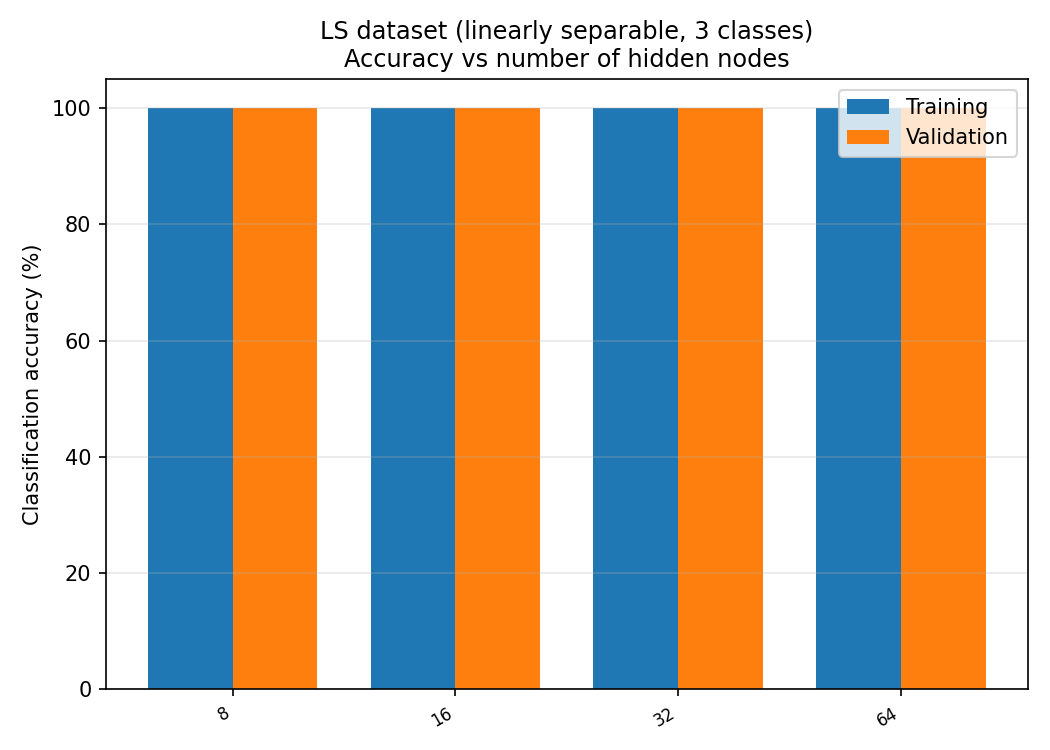
\includegraphics[width=0.78\textwidth,height=7.6cm,keepaspectratio]{figures/classification_ls__model_selection_accuracy.png}
\caption{Training and validation accuracy against the number of hidden nodes.}
\end{figure}

Average error against epochs for each architecture that was tried, one graph per architecture. They are deliberately not overlaid on a single axis: with several architectures the curves sit on top of one another and none of them can be read.

\begin{figure}[H]
\centering
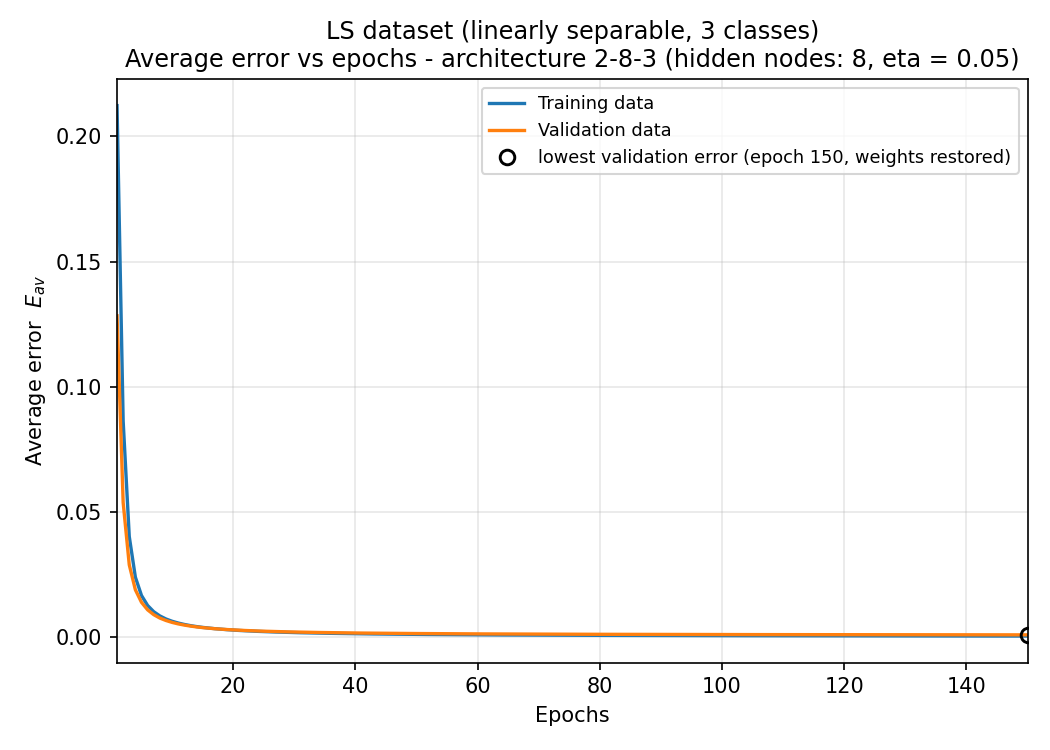
\includegraphics[width=0.78\textwidth,height=7.4cm,keepaspectratio]{figures/classification_ls__error_curves__hidden_8.png}
\caption{Average error against epochs, architecture 2-8-3 (hidden nodes: 8).}
\end{figure}

\begin{figure}[H]
\centering
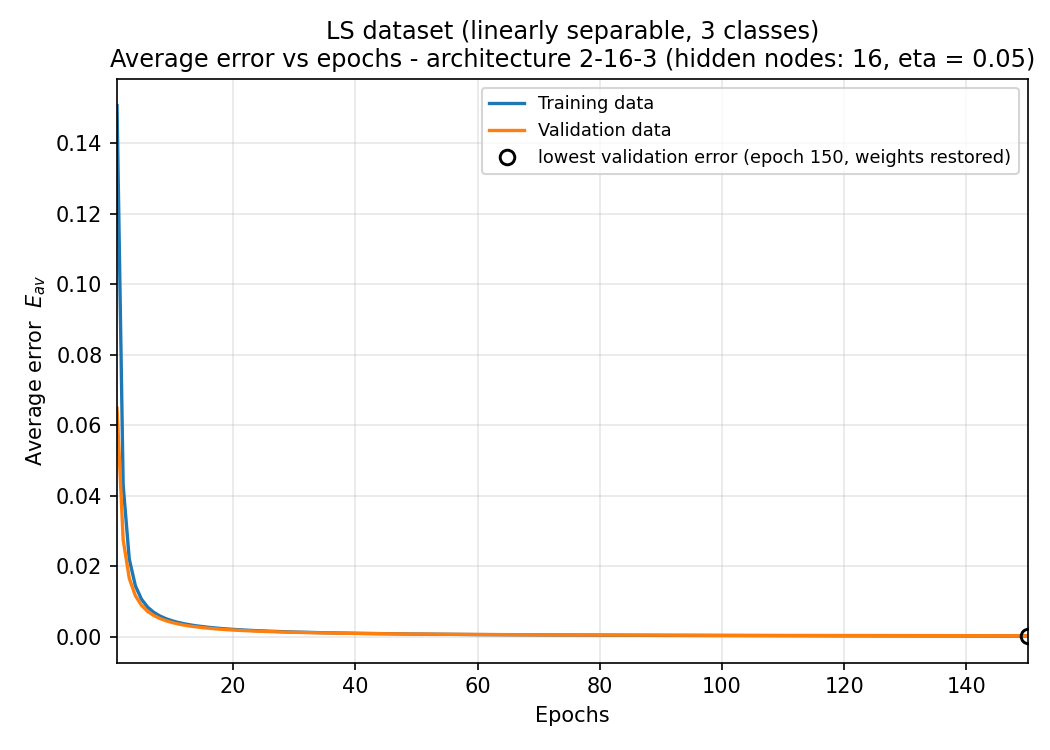
\includegraphics[width=0.78\textwidth,height=7.4cm,keepaspectratio]{figures/classification_ls__error_curves__hidden_16.png}
\caption{Average error against epochs, architecture 2-16-3 (hidden nodes: 16).}
\end{figure}

\begin{figure}[H]
\centering
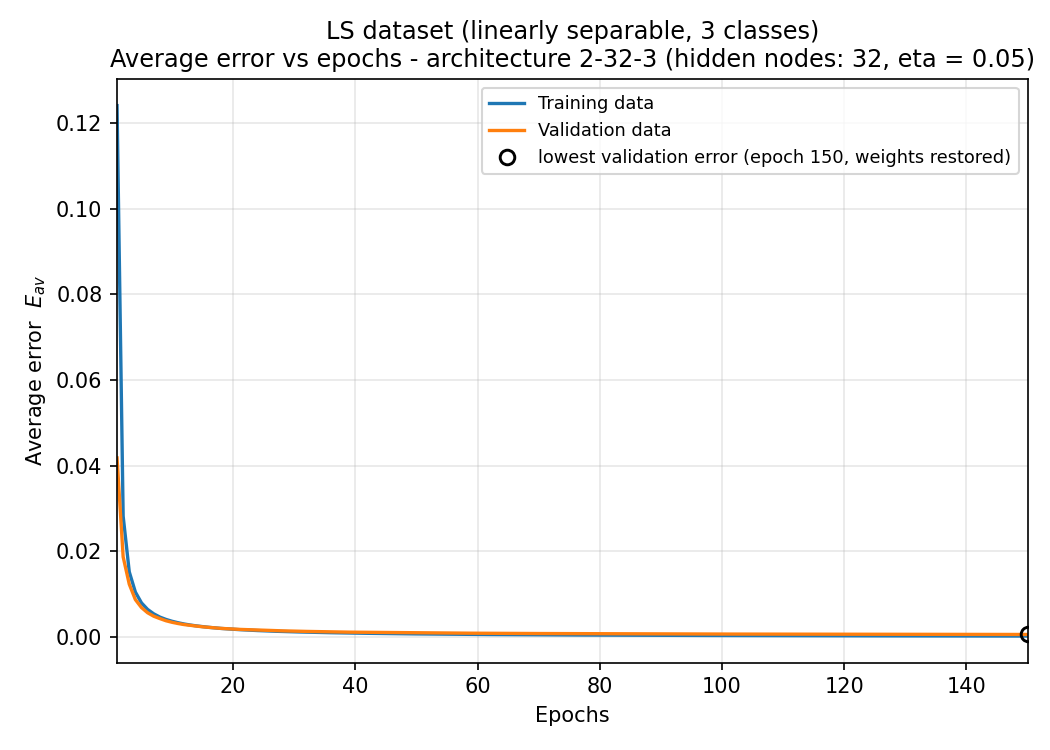
\includegraphics[width=0.78\textwidth,height=7.4cm,keepaspectratio]{figures/classification_ls__error_curves__hidden_32.png}
\caption{Average error against epochs, architecture 2-32-3 (hidden nodes: 32).}
\end{figure}

\begin{figure}[H]
\centering
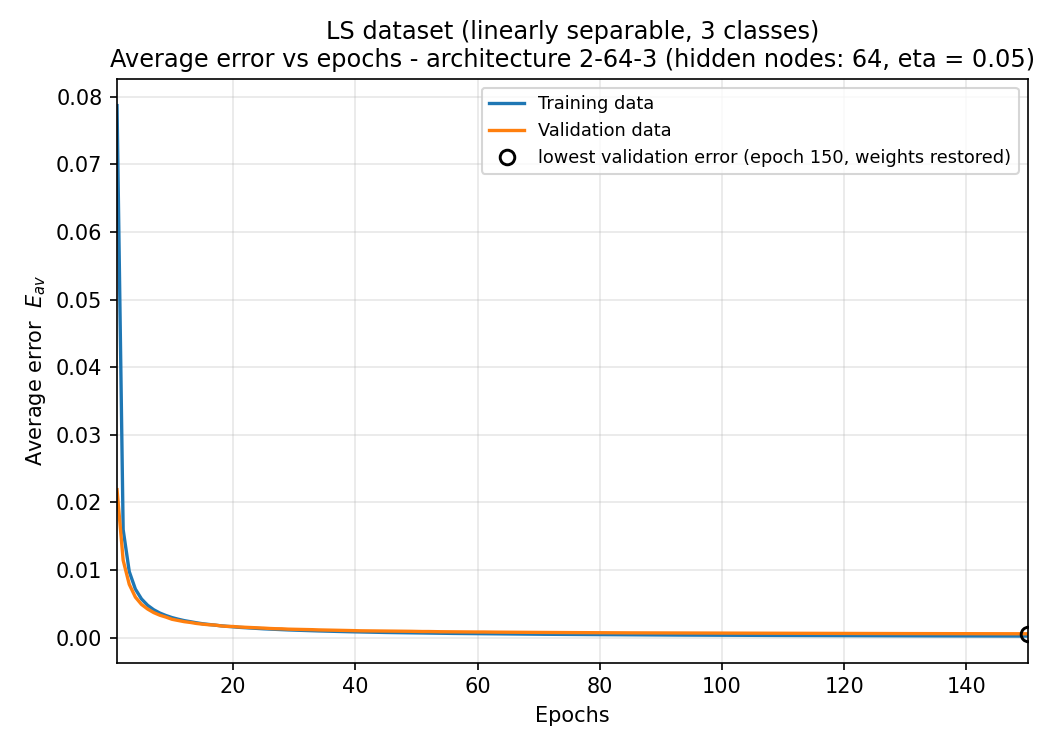
\includegraphics[width=0.78\textwidth,height=7.4cm,keepaspectratio]{figures/classification_ls__error_curves__hidden_64.png}
\caption{Average error against epochs, architecture 2-64-3 (hidden nodes: 64).}
\end{figure}

\clearpage

\subsection{Confusion Matrix and Per-Class Metrics on Validation Data, for Every Architecture}
\noindent\textbf{Architecture 2-8-3 (hidden nodes 8)} --- classification accuracy = \textbf{100.00\%}

\vspace{2pt}
\noindent
\begin{minipage}[t]{0.42\textwidth}\footnotesize\centering
\begin{tabular}{lrrr}
\toprule
 & \textbf{Pred 1} & \textbf{Pred 2} & \textbf{Pred 3} \\
\midrule
\textbf{True 1} & 100 & 0 & 0 \\
\textbf{True 2} & 0 & 100 & 0 \\
\textbf{True 3} & 0 & 0 & 100 \\
\bottomrule
\end{tabular}
\end{minipage}\hfill
\begin{minipage}[t]{0.56\textwidth}\footnotesize\centering
\begin{tabular}{lrrr}
\toprule
\textbf{Class} & \textbf{Precision} & \textbf{Recall} & \textbf{F-measure} \\
\midrule
1 & 1.0000 & 1.0000 & 1.0000 \\
2 & 1.0000 & 1.0000 & 1.0000 \\
3 & 1.0000 & 1.0000 & 1.0000 \\
\midrule
\textbf{Mean} & 1.0000 & 1.0000 & 1.0000 \\
\bottomrule
\end{tabular}
\end{minipage}

\vspace{8pt}

\noindent\textbf{Architecture 2-16-3 (hidden nodes 16) (selected)} --- classification accuracy = \textbf{100.00\%}

\vspace{2pt}
\noindent
\begin{minipage}[t]{0.42\textwidth}\footnotesize\centering
\begin{tabular}{lrrr}
\toprule
 & \textbf{Pred 1} & \textbf{Pred 2} & \textbf{Pred 3} \\
\midrule
\textbf{True 1} & 100 & 0 & 0 \\
\textbf{True 2} & 0 & 100 & 0 \\
\textbf{True 3} & 0 & 0 & 100 \\
\bottomrule
\end{tabular}
\end{minipage}\hfill
\begin{minipage}[t]{0.56\textwidth}\footnotesize\centering
\begin{tabular}{lrrr}
\toprule
\textbf{Class} & \textbf{Precision} & \textbf{Recall} & \textbf{F-measure} \\
\midrule
1 & 1.0000 & 1.0000 & 1.0000 \\
2 & 1.0000 & 1.0000 & 1.0000 \\
3 & 1.0000 & 1.0000 & 1.0000 \\
\midrule
\textbf{Mean} & 1.0000 & 1.0000 & 1.0000 \\
\bottomrule
\end{tabular}
\end{minipage}

\vspace{8pt}

\noindent\textbf{Architecture 2-32-3 (hidden nodes 32)} --- classification accuracy = \textbf{100.00\%}

\vspace{2pt}
\noindent
\begin{minipage}[t]{0.42\textwidth}\footnotesize\centering
\begin{tabular}{lrrr}
\toprule
 & \textbf{Pred 1} & \textbf{Pred 2} & \textbf{Pred 3} \\
\midrule
\textbf{True 1} & 100 & 0 & 0 \\
\textbf{True 2} & 0 & 100 & 0 \\
\textbf{True 3} & 0 & 0 & 100 \\
\bottomrule
\end{tabular}
\end{minipage}\hfill
\begin{minipage}[t]{0.56\textwidth}\footnotesize\centering
\begin{tabular}{lrrr}
\toprule
\textbf{Class} & \textbf{Precision} & \textbf{Recall} & \textbf{F-measure} \\
\midrule
1 & 1.0000 & 1.0000 & 1.0000 \\
2 & 1.0000 & 1.0000 & 1.0000 \\
3 & 1.0000 & 1.0000 & 1.0000 \\
\midrule
\textbf{Mean} & 1.0000 & 1.0000 & 1.0000 \\
\bottomrule
\end{tabular}
\end{minipage}

\vspace{8pt}

\noindent\textbf{Architecture 2-64-3 (hidden nodes 64)} --- classification accuracy = \textbf{100.00\%}

\vspace{2pt}
\noindent
\begin{minipage}[t]{0.42\textwidth}\footnotesize\centering
\begin{tabular}{lrrr}
\toprule
 & \textbf{Pred 1} & \textbf{Pred 2} & \textbf{Pred 3} \\
\midrule
\textbf{True 1} & 100 & 0 & 0 \\
\textbf{True 2} & 0 & 100 & 0 \\
\textbf{True 3} & 0 & 0 & 100 \\
\bottomrule
\end{tabular}
\end{minipage}\hfill
\begin{minipage}[t]{0.56\textwidth}\footnotesize\centering
\begin{tabular}{lrrr}
\toprule
\textbf{Class} & \textbf{Precision} & \textbf{Recall} & \textbf{F-measure} \\
\midrule
1 & 1.0000 & 1.0000 & 1.0000 \\
2 & 1.0000 & 1.0000 & 1.0000 \\
3 & 1.0000 & 1.0000 & 1.0000 \\
\midrule
\textbf{Mean} & 1.0000 & 1.0000 & 1.0000 \\
\bottomrule
\end{tabular}
\end{minipage}

\vspace{8pt}

\clearpage

\subsection{Best Architecture: 2-16-3}
The architecture selected on the validation set is \textbf{2-16-3} (hidden nodes: 16), trained for 150 epochs. All the plots below are for this model.

\parahead{Average error against epochs.}
\begin{figure}[H]
\centering
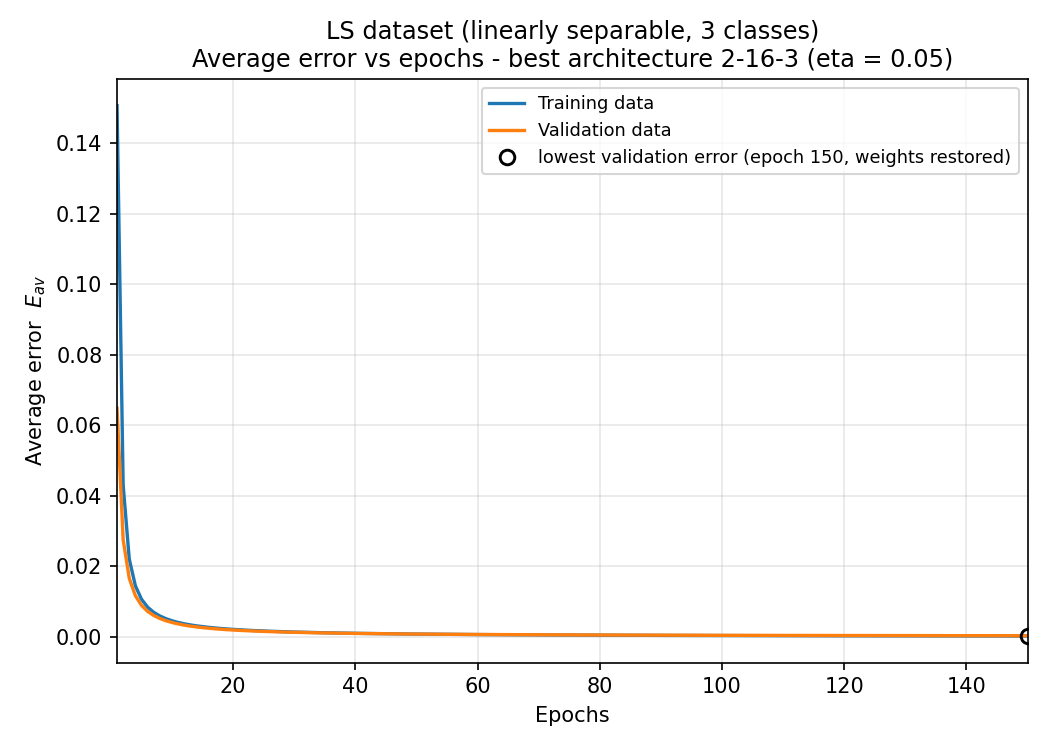
\includegraphics[width=0.8\textwidth,height=8.4cm,keepaspectratio]{figures/classification_ls__best_architecture__error_vs_epochs.png}
\caption{Average error $E_{\mathrm{av}}$ against epochs for the best architecture.}
\end{figure}

\parahead{Decision region superimposed on the training data.}
\begin{figure}[H]
\centering
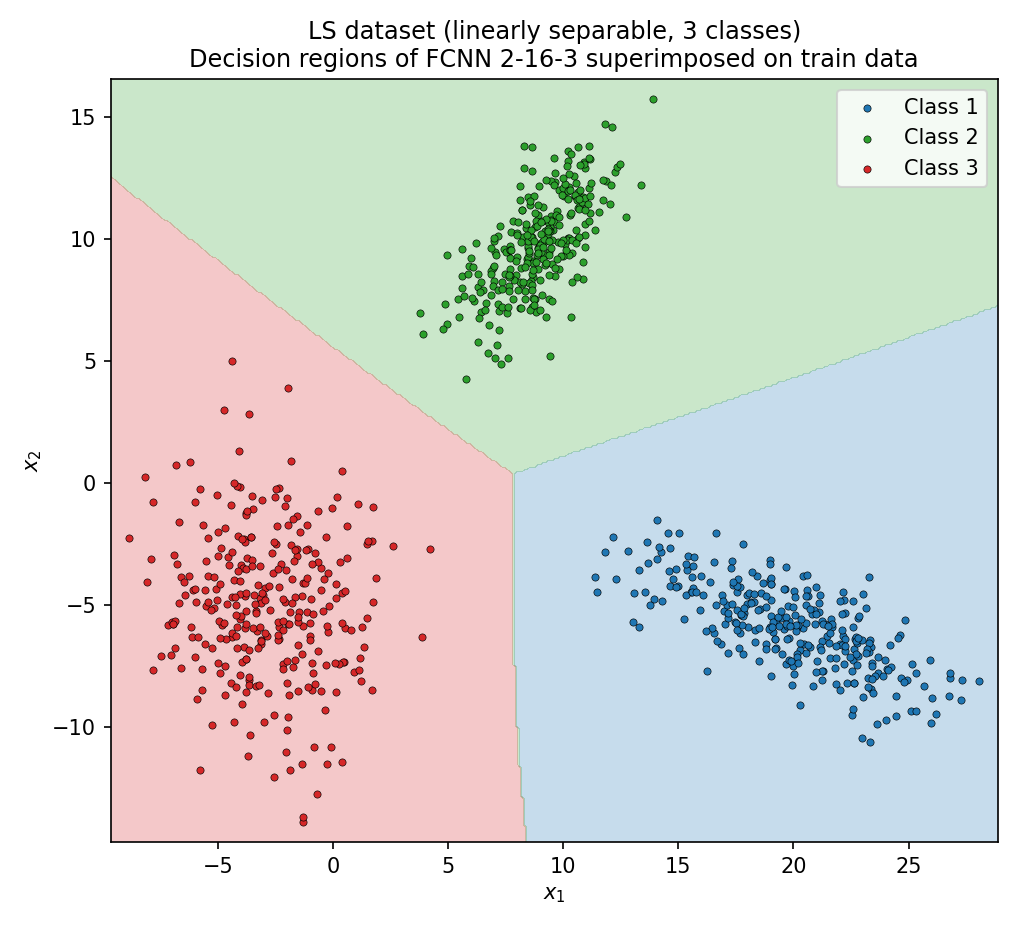
\includegraphics[width=0.82\textwidth,height=10.5cm,keepaspectratio]{figures/classification_ls__best_architecture__decision_region_train.png}
\caption{Decision regions of the best FCNN, superimposed on the training data.}
\end{figure}

\clearpage

\paragraph{Confusion matrix and metrics for the best architecture.}

\noindent\textbf{Training data} --- classification accuracy = \textbf{100.00\%}

\vspace{2pt}
\noindent
\begin{minipage}[t]{0.42\textwidth}\footnotesize\centering
\begin{tabular}{lrrr}
\toprule
 & \textbf{Pred 1} & \textbf{Pred 2} & \textbf{Pred 3} \\
\midrule
\textbf{True 1} & 300 & 0 & 0 \\
\textbf{True 2} & 0 & 300 & 0 \\
\textbf{True 3} & 0 & 0 & 300 \\
\bottomrule
\end{tabular}
\end{minipage}\hfill
\begin{minipage}[t]{0.56\textwidth}\footnotesize\centering
\begin{tabular}{lrrr}
\toprule
\textbf{Class} & \textbf{Precision} & \textbf{Recall} & \textbf{F-measure} \\
\midrule
1 & 1.0000 & 1.0000 & 1.0000 \\
2 & 1.0000 & 1.0000 & 1.0000 \\
3 & 1.0000 & 1.0000 & 1.0000 \\
\midrule
\textbf{Mean} & 1.0000 & 1.0000 & 1.0000 \\
\bottomrule
\end{tabular}
\end{minipage}

\vspace{8pt}

\noindent\textbf{Validation data} --- classification accuracy = \textbf{100.00\%}

\vspace{2pt}
\noindent
\begin{minipage}[t]{0.42\textwidth}\footnotesize\centering
\begin{tabular}{lrrr}
\toprule
 & \textbf{Pred 1} & \textbf{Pred 2} & \textbf{Pred 3} \\
\midrule
\textbf{True 1} & 100 & 0 & 0 \\
\textbf{True 2} & 0 & 100 & 0 \\
\textbf{True 3} & 0 & 0 & 100 \\
\bottomrule
\end{tabular}
\end{minipage}\hfill
\begin{minipage}[t]{0.56\textwidth}\footnotesize\centering
\begin{tabular}{lrrr}
\toprule
\textbf{Class} & \textbf{Precision} & \textbf{Recall} & \textbf{F-measure} \\
\midrule
1 & 1.0000 & 1.0000 & 1.0000 \\
2 & 1.0000 & 1.0000 & 1.0000 \\
3 & 1.0000 & 1.0000 & 1.0000 \\
\midrule
\textbf{Mean} & 1.0000 & 1.0000 & 1.0000 \\
\bottomrule
\end{tabular}
\end{minipage}

\vspace{8pt}

\noindent\textbf{Test data} --- classification accuracy = \textbf{100.00\%}

\vspace{2pt}
\noindent
\begin{minipage}[t]{0.42\textwidth}\footnotesize\centering
\begin{tabular}{lrrr}
\toprule
 & \textbf{Pred 1} & \textbf{Pred 2} & \textbf{Pred 3} \\
\midrule
\textbf{True 1} & 100 & 0 & 0 \\
\textbf{True 2} & 0 & 100 & 0 \\
\textbf{True 3} & 0 & 0 & 100 \\
\bottomrule
\end{tabular}
\end{minipage}\hfill
\begin{minipage}[t]{0.56\textwidth}\footnotesize\centering
\begin{tabular}{lrrr}
\toprule
\textbf{Class} & \textbf{Precision} & \textbf{Recall} & \textbf{F-measure} \\
\midrule
1 & 1.0000 & 1.0000 & 1.0000 \\
2 & 1.0000 & 1.0000 & 1.0000 \\
3 & 1.0000 & 1.0000 & 1.0000 \\
\midrule
\textbf{Mean} & 1.0000 & 1.0000 & 1.0000 \\
\bottomrule
\end{tabular}
\end{minipage}

\vspace{8pt}

\clearpage

\subsection{Outputs of the Hidden Nodes and Output Nodes}
Every hidden node and every output node is plotted in its own figure: the two axes in the base plane are the input variables $x_{1}$ and $x_{2}$ of each example and the vertical axis is the output of that node. The selected network has 19 nodes in total, so the complete set is 57 figures (one per node per split); they are all written to \texttt{outputs/\allowbreak classification\_\allowbreak ls/\allowbreak best\_\allowbreak architecture/\allowbreak node\_\allowbreak outputs/\allowbreak }. The first 6 nodes of each layer are reproduced below for each split.

\parahead{Hidden layer 1 --- train data.}
\begin{figure}[H]
\centering
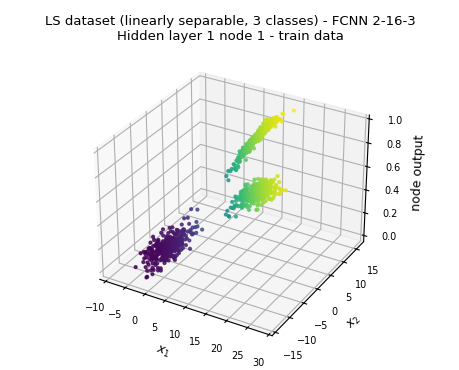
\includegraphics[width=0.323\textwidth]{figures/classification_ls__best_architecture__node_outputs__hidden_layer1__train__node_001.png}\hfill%
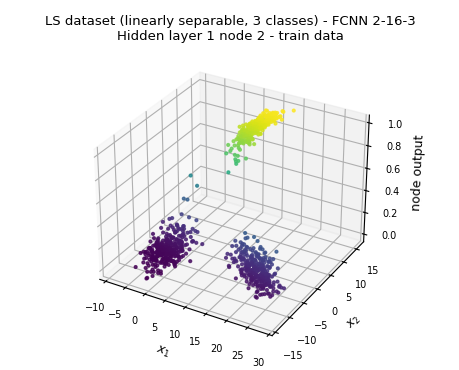
\includegraphics[width=0.323\textwidth]{figures/classification_ls__best_architecture__node_outputs__hidden_layer1__train__node_002.png}\hfill%
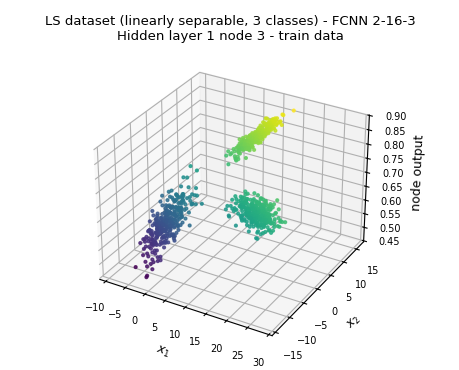
\includegraphics[width=0.323\textwidth]{figures/classification_ls__best_architecture__node_outputs__hidden_layer1__train__node_003.png}\\[4pt]%
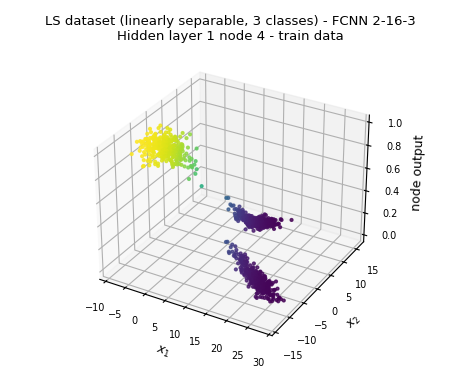
\includegraphics[width=0.323\textwidth]{figures/classification_ls__best_architecture__node_outputs__hidden_layer1__train__node_004.png}\hfill%
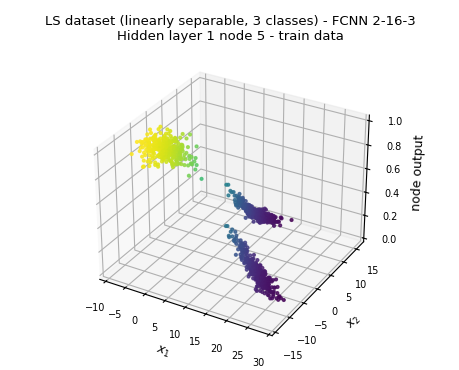
\includegraphics[width=0.323\textwidth]{figures/classification_ls__best_architecture__node_outputs__hidden_layer1__train__node_005.png}\hfill%
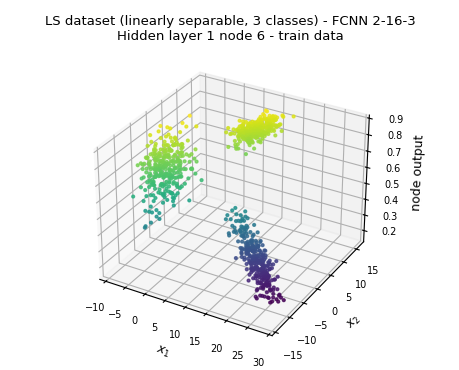
\includegraphics[width=0.323\textwidth]{figures/classification_ls__best_architecture__node_outputs__hidden_layer1__train__node_006.png}
\caption{Outputs of hidden layer 1 nodes 1--6 of 16 (train data). Each node has its own figure; all 16 are in \texttt{outputs/\allowbreak classification\_\allowbreak ls/\allowbreak best\_\allowbreak architecture/\allowbreak node\_\allowbreak outputs/\allowbreak hidden\_\allowbreak layer1/\allowbreak train/\allowbreak }.}
\end{figure}

\parahead{Hidden layer 1 --- val data.}
\begin{figure}[H]
\centering
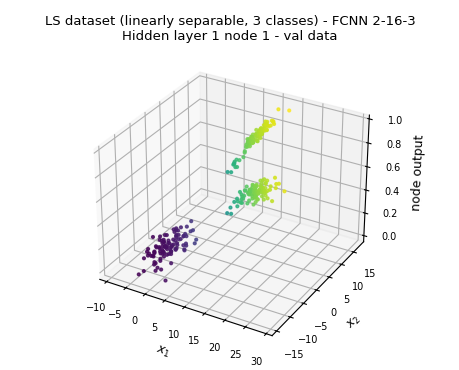
\includegraphics[width=0.323\textwidth]{figures/classification_ls__best_architecture__node_outputs__hidden_layer1__val__node_001.png}\hfill%
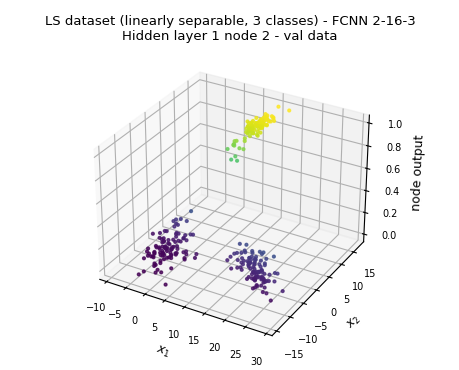
\includegraphics[width=0.323\textwidth]{figures/classification_ls__best_architecture__node_outputs__hidden_layer1__val__node_002.png}\hfill%
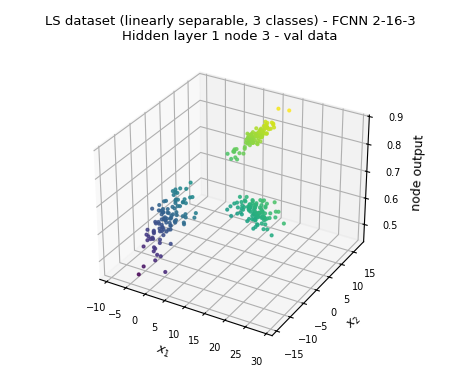
\includegraphics[width=0.323\textwidth]{figures/classification_ls__best_architecture__node_outputs__hidden_layer1__val__node_003.png}\\[4pt]%
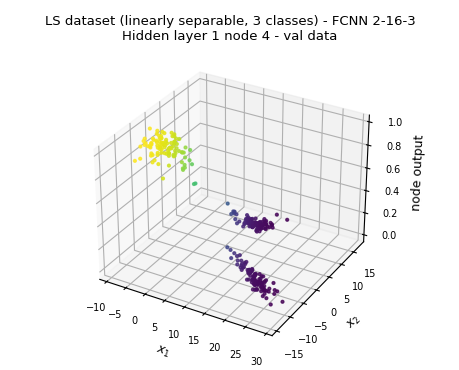
\includegraphics[width=0.323\textwidth]{figures/classification_ls__best_architecture__node_outputs__hidden_layer1__val__node_004.png}\hfill%
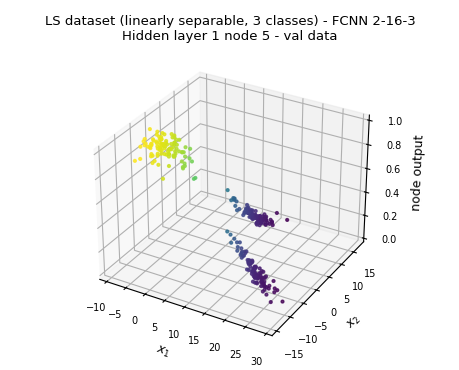
\includegraphics[width=0.323\textwidth]{figures/classification_ls__best_architecture__node_outputs__hidden_layer1__val__node_005.png}\hfill%
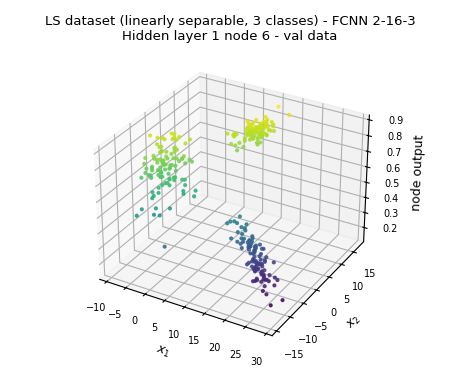
\includegraphics[width=0.323\textwidth]{figures/classification_ls__best_architecture__node_outputs__hidden_layer1__val__node_006.png}
\caption{Outputs of hidden layer 1 nodes 1--6 of 16 (val data). Each node has its own figure; all 16 are in \texttt{outputs/\allowbreak classification\_\allowbreak ls/\allowbreak best\_\allowbreak architecture/\allowbreak node\_\allowbreak outputs/\allowbreak hidden\_\allowbreak layer1/\allowbreak val/\allowbreak }.}
\end{figure}

\parahead{Hidden layer 1 --- test data.}
\begin{figure}[H]
\centering
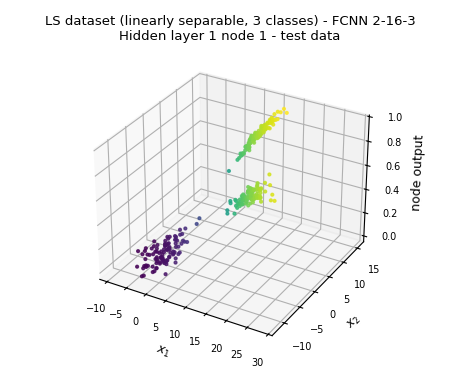
\includegraphics[width=0.323\textwidth]{figures/classification_ls__best_architecture__node_outputs__hidden_layer1__test__node_001.png}\hfill%
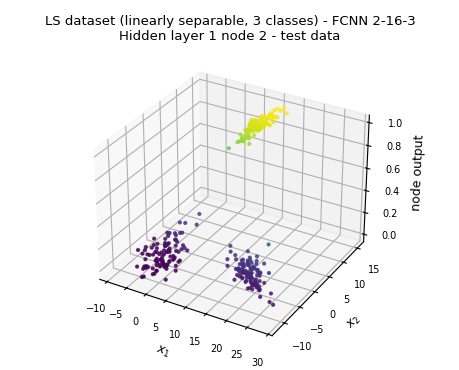
\includegraphics[width=0.323\textwidth]{figures/classification_ls__best_architecture__node_outputs__hidden_layer1__test__node_002.png}\hfill%
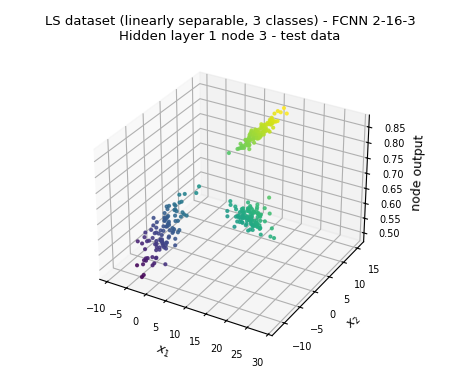
\includegraphics[width=0.323\textwidth]{figures/classification_ls__best_architecture__node_outputs__hidden_layer1__test__node_003.png}\\[4pt]%
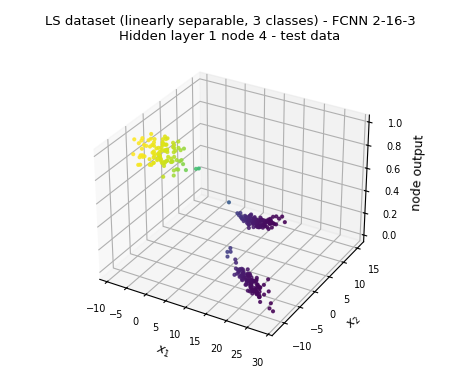
\includegraphics[width=0.323\textwidth]{figures/classification_ls__best_architecture__node_outputs__hidden_layer1__test__node_004.png}\hfill%
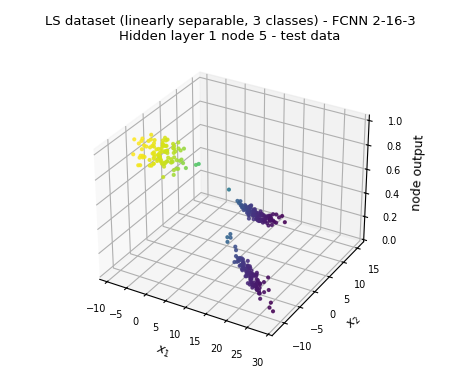
\includegraphics[width=0.323\textwidth]{figures/classification_ls__best_architecture__node_outputs__hidden_layer1__test__node_005.png}\hfill%
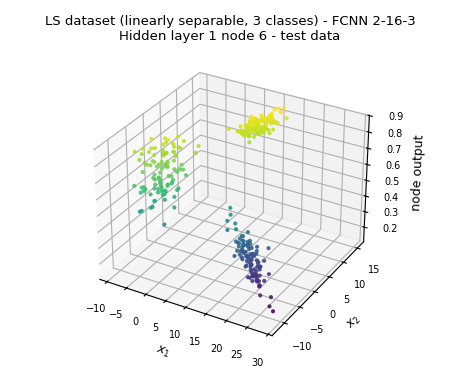
\includegraphics[width=0.323\textwidth]{figures/classification_ls__best_architecture__node_outputs__hidden_layer1__test__node_006.png}
\caption{Outputs of hidden layer 1 nodes 1--6 of 16 (test data). Each node has its own figure; all 16 are in \texttt{outputs/\allowbreak classification\_\allowbreak ls/\allowbreak best\_\allowbreak architecture/\allowbreak node\_\allowbreak outputs/\allowbreak hidden\_\allowbreak layer1/\allowbreak test/\allowbreak }.}
\end{figure}

\clearpage

\parahead{Output layer --- train data.}
\begin{figure}[H]
\centering
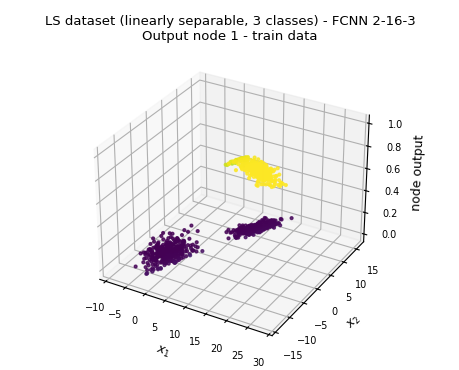
\includegraphics[width=0.323\textwidth]{figures/classification_ls__best_architecture__node_outputs__output_layer__train__node_001.png}\hfill%
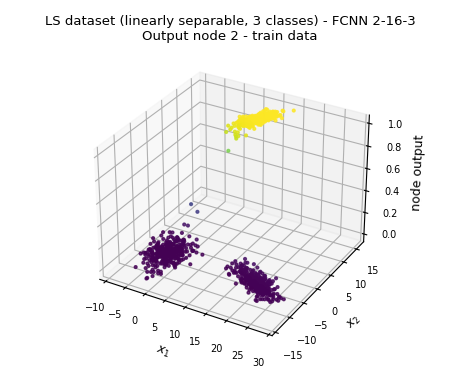
\includegraphics[width=0.323\textwidth]{figures/classification_ls__best_architecture__node_outputs__output_layer__train__node_002.png}\hfill%
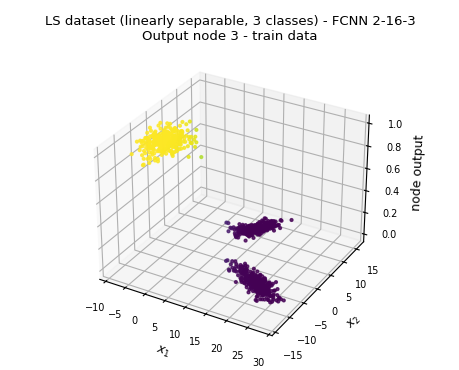
\includegraphics[width=0.323\textwidth]{figures/classification_ls__best_architecture__node_outputs__output_layer__train__node_003.png}
\caption{Outputs of all 3 output nodes (train data), one figure per node.}
\end{figure}

\parahead{Output layer --- val data.}
\begin{figure}[H]
\centering
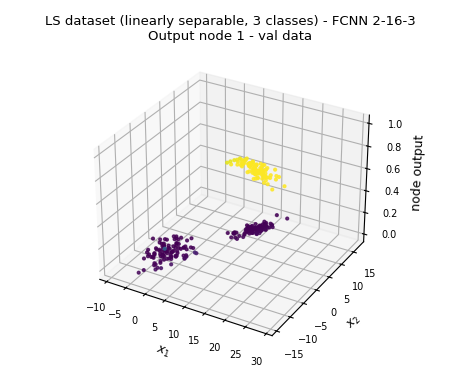
\includegraphics[width=0.323\textwidth]{figures/classification_ls__best_architecture__node_outputs__output_layer__val__node_001.png}\hfill%
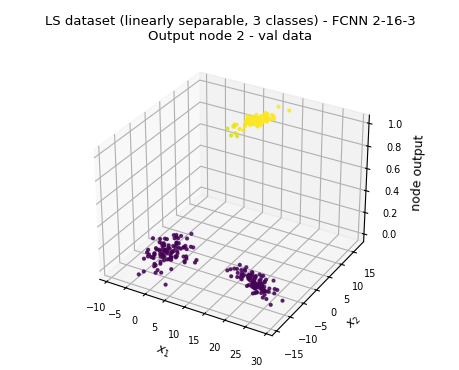
\includegraphics[width=0.323\textwidth]{figures/classification_ls__best_architecture__node_outputs__output_layer__val__node_002.png}\hfill%
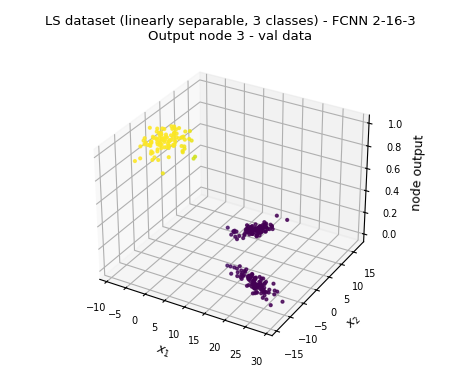
\includegraphics[width=0.323\textwidth]{figures/classification_ls__best_architecture__node_outputs__output_layer__val__node_003.png}
\caption{Outputs of all 3 output nodes (val data), one figure per node.}
\end{figure}

\parahead{Output layer --- test data.}
\begin{figure}[H]
\centering
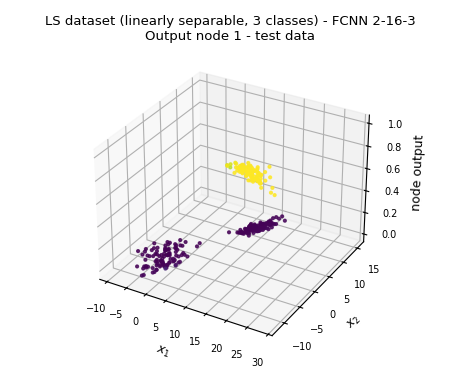
\includegraphics[width=0.323\textwidth]{figures/classification_ls__best_architecture__node_outputs__output_layer__test__node_001.png}\hfill%
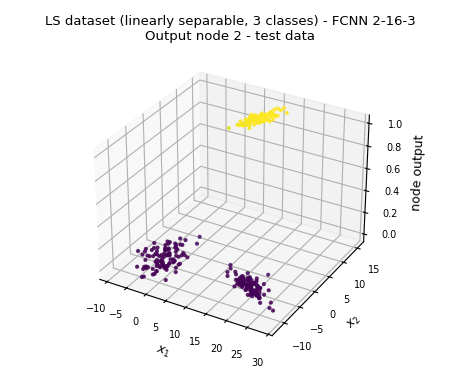
\includegraphics[width=0.323\textwidth]{figures/classification_ls__best_architecture__node_outputs__output_layer__test__node_002.png}\hfill%
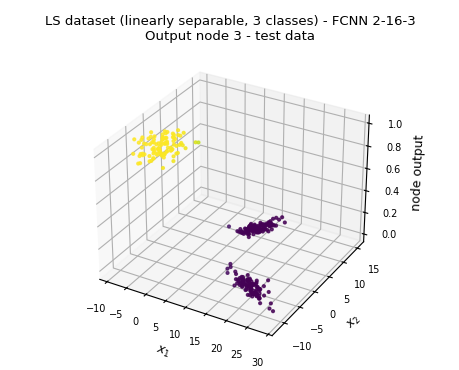
\includegraphics[width=0.323\textwidth]{figures/classification_ls__best_architecture__node_outputs__output_layer__test__node_003.png}
\caption{Outputs of all 3 output nodes (test data), one figure per node.}
\end{figure}

\clearpage

\subsection{Comparison with the Single-Neuron Model (Assignment-1)}
The Assignment-1 model --- one perceptron per pair of classes, combined by one-against-one majority voting --- was retrained on exactly the same 60/20/20 split and scored with the same from-scratch metric code, so the two rows below are directly comparable.

\begin{table}[H]
\centering
\caption{FCNN against the Assignment-1 single-neuron model.}
\setlength{\tabcolsep}{4pt}
\footnotesize
\resizebox{\textwidth}{!}{%
\begin{tabular}{lrrrrr}
\toprule
\textbf{Model} & \textbf{Val acc.\%} & \textbf{Test acc.\%} & \textbf{Test mean prec.} & \textbf{Test mean recall} & \textbf{Test mean $F$} \\
\midrule
Single neuron (one-against-one perceptron) & 100.00 & 100.00 & 1.0000 & 1.0000 & 1.0000 \\
\rowcolor{bestrow} \textbf{FCNN 2-16-3 (Assignment-2)} & \textbf{100.00} & \textbf{100.00} & \textbf{1.0000} & \textbf{1.0000} & \textbf{1.0000} \\
\bottomrule
\end{tabular}
}
\end{table}

\begin{figure}[H]
\centering
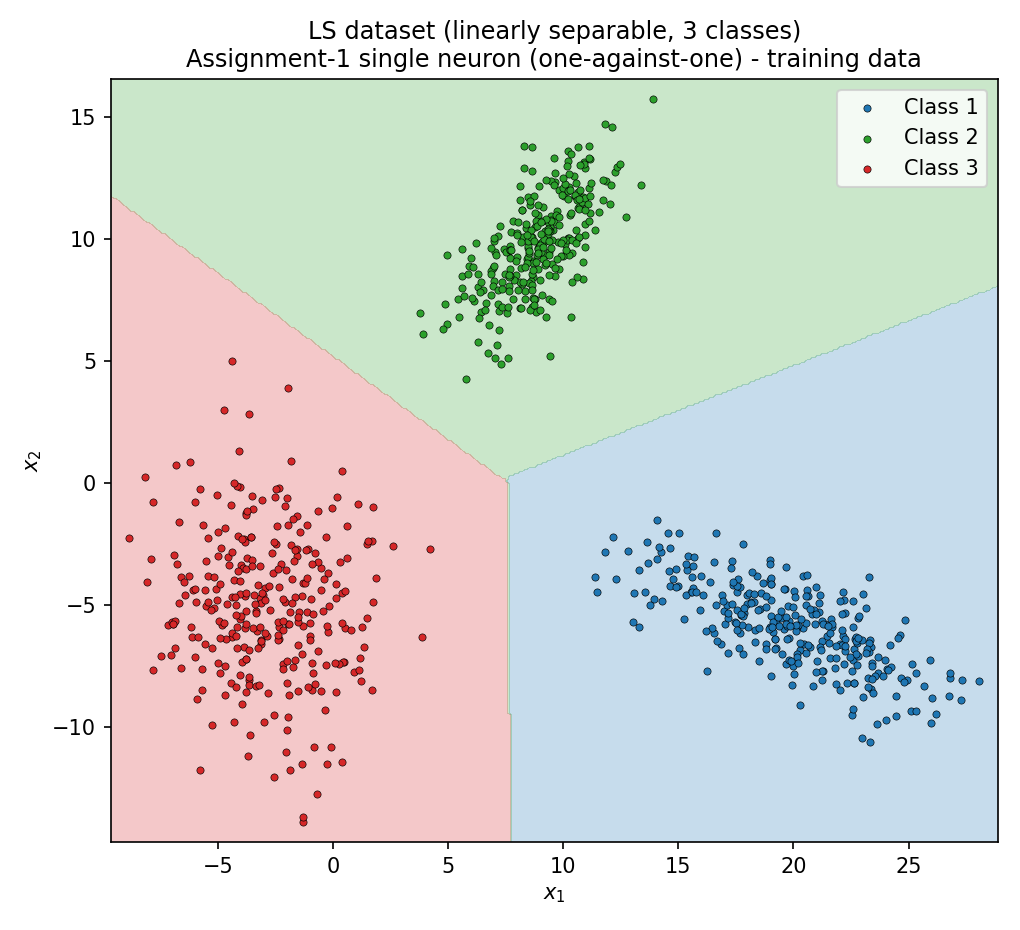
\includegraphics[width=0.8\textwidth,height=9.6cm,keepaspectratio]{figures/classification_ls__baseline_single_neuron_decision_region_train.png}
\caption{Decision regions of the Assignment-1 single-neuron model on the same training data.}
\end{figure}

\subsection{Inferences}
\begin{itemize}
  \item The three classes of the LS dataset form compact, well-separated clusters, so every architecture that was tried reached 100.00\% validation accuracy, and the accuracies tie.
  \item In terms of classification accuracy alone the small network 2-8-3 (51 weights) is already sufficient, and by Occam's razor it is the model one would deploy: beyond it, extra hidden nodes add parameters without adding accuracy. The architecture reported as "best" (2-16-3) is the one the selection rule returns because, among those tied on accuracy, it has the smallest validation average error - its output activations sit closest to the 1-of-K targets.
  \item The single neuron of Assignment-1 also achieves 100.00\% on this test data (+0.00 percentage points difference against the FCNN). This is the important negative result of this dataset: when the classes are linearly separable, the extra representational power of hidden layers buys nothing, and the simpler model should be preferred.
  \item The decision-region plot shows almost straight boundaries meeting near the centre of the input space. Although the FCNN \textit{can} bend its boundaries, training drives it to an essentially piecewise-linear solution, because that is already enough to drive the squared error to a very small value.
  \item The hidden-node output plots show sigmoid ridges oriented in different directions: each hidden node is effectively a soft linear discriminant, and the output layer recombines a small number of them. Several hidden nodes in the larger networks produce almost the same surface, i.e. they are redundant.
  \item The average-error curve of the best architecture falls steeply during the first epochs and then flattens; training ran for 150 epochs before the convergence criterion stopped it. Training and validation curves stay close together, so there is no sign of overfitting at this network size.
  \item Training, validation and test metrics of the selected model agree closely, which is what one expects when the model is selected on data that is disjoint from the test set and the three splits are drawn from the same distribution.
\end{itemize}

\clearpage

\section{Classification --- Dataset 2 (NLS, Nonlinearly Separable)}
Model: an FCNN with two hidden layers, logistic hidden and output nodes, three output nodes with $1$-of-$K$ coded targets, trained by SGD backpropagation with the squared-error loss and learning rate $\eta = 0.05$. 4 architectures were trained and compared on the validation set.

\subsection{Results for the Different Architectures (Validation Data)}
\begin{table}[H]
\centering
\caption{Validation-set performance of every architecture that was tried. The selected architecture is highlighted.}
\setlength{\tabcolsep}{4pt}
\footnotesize
\resizebox{\textwidth}{!}{%
\begin{tabular}{llrrrrrrr}
\toprule
\textbf{Hidden nodes} & \textbf{Architecture} & \textbf{Params} & \textbf{Epochs} & \textbf{Train acc.\%} & \textbf{Val acc.\%} & \textbf{Mean prec.} & \textbf{Mean recall} & \textbf{Mean $F$} \\
\midrule
16-8 & 2-16-8-3 & 211 & 300 & 100.00 & 100.00 & 1.0000 & 1.0000 & 1.0000 \\
32-16 & 2-32-16-3 & 675 & 300 & 100.00 & 100.00 & 1.0000 & 1.0000 & 1.0000 \\
\rowcolor{bestrow} \textbf{64-16} & \textbf{2-64-16-3} & \textbf{1283} & \textbf{300} & \textbf{100.00} & \textbf{100.00} & \textbf{1.0000} & \textbf{1.0000} & \textbf{1.0000} \\
64-32 & 2-64-32-3 & 2371 & 300 & 100.00 & 100.00 & 1.0000 & 1.0000 & 1.0000 \\
\bottomrule
\end{tabular}
}
\end{table}

\begin{figure}[H]
\centering
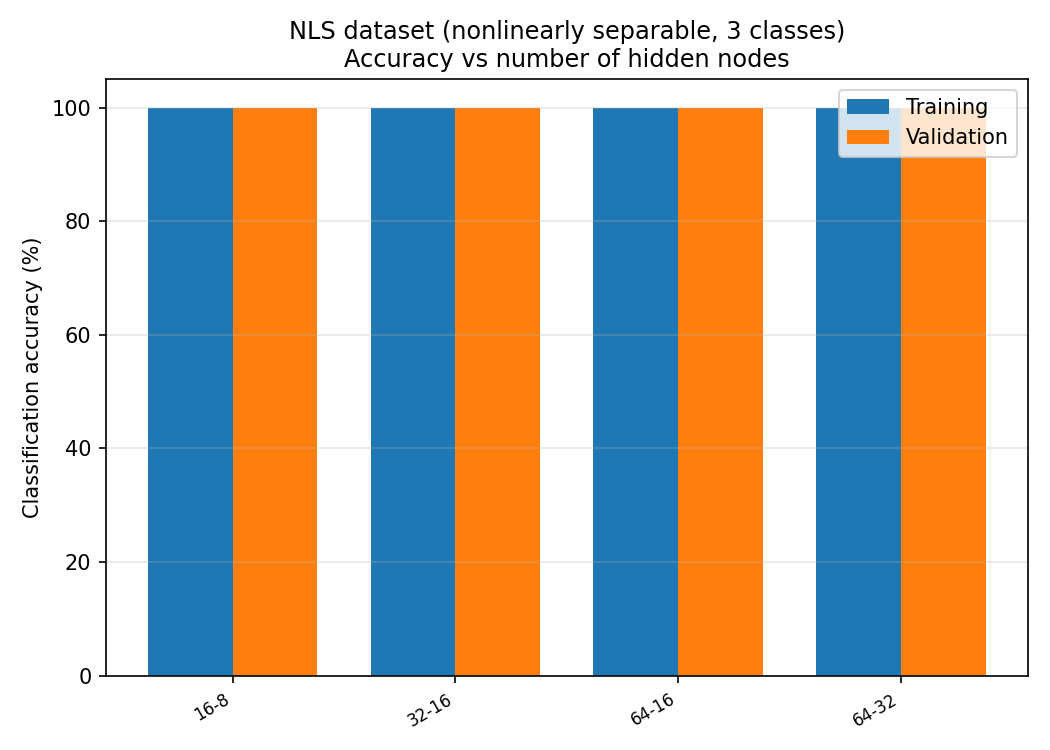
\includegraphics[width=0.78\textwidth,height=7.6cm,keepaspectratio]{figures/classification_nls__model_selection_accuracy.png}
\caption{Training and validation accuracy against the number of hidden nodes.}
\end{figure}

Average error against epochs for each architecture that was tried, one graph per architecture. They are deliberately not overlaid on a single axis: with several architectures the curves sit on top of one another and none of them can be read.

\begin{figure}[H]
\centering
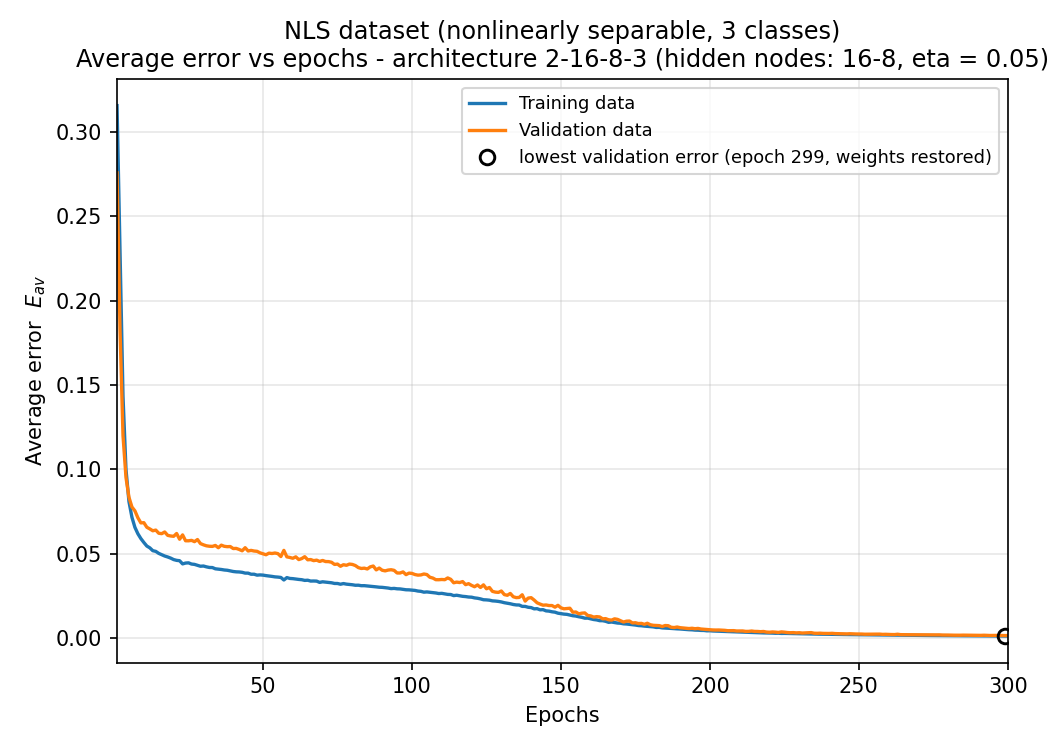
\includegraphics[width=0.78\textwidth,height=7.4cm,keepaspectratio]{figures/classification_nls__error_curves__hidden_16-8.png}
\caption{Average error against epochs, architecture 2-16-8-3 (hidden nodes: 16-8).}
\end{figure}

\begin{figure}[H]
\centering
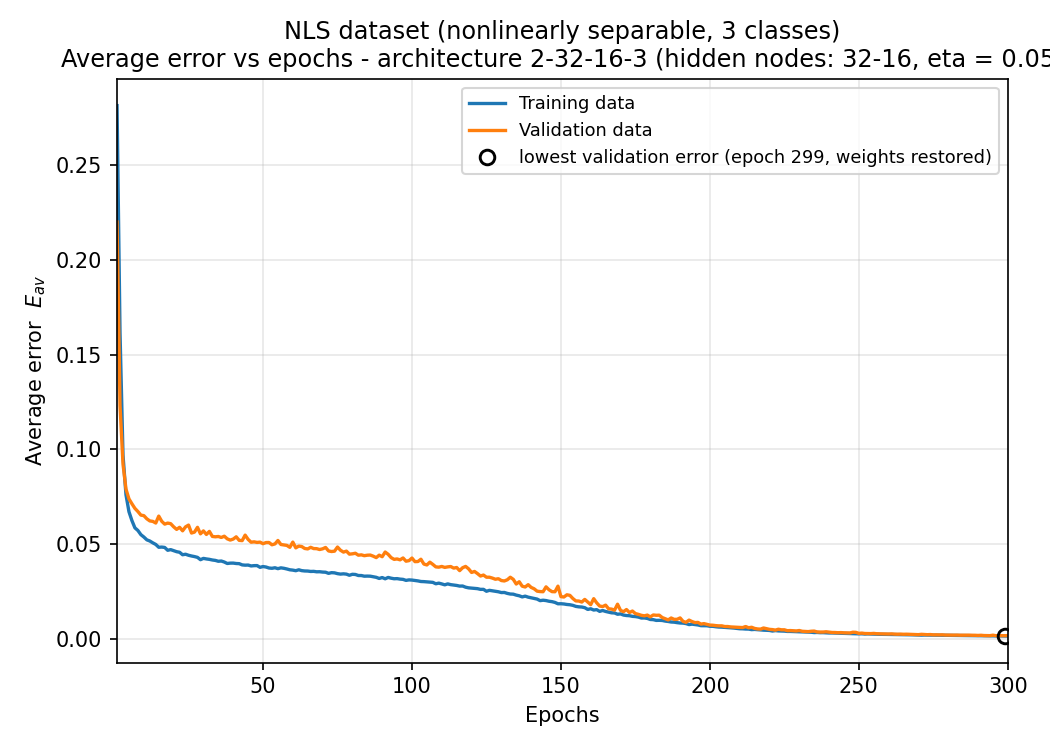
\includegraphics[width=0.78\textwidth,height=7.4cm,keepaspectratio]{figures/classification_nls__error_curves__hidden_32-16.png}
\caption{Average error against epochs, architecture 2-32-16-3 (hidden nodes: 32-16).}
\end{figure}

\begin{figure}[H]
\centering
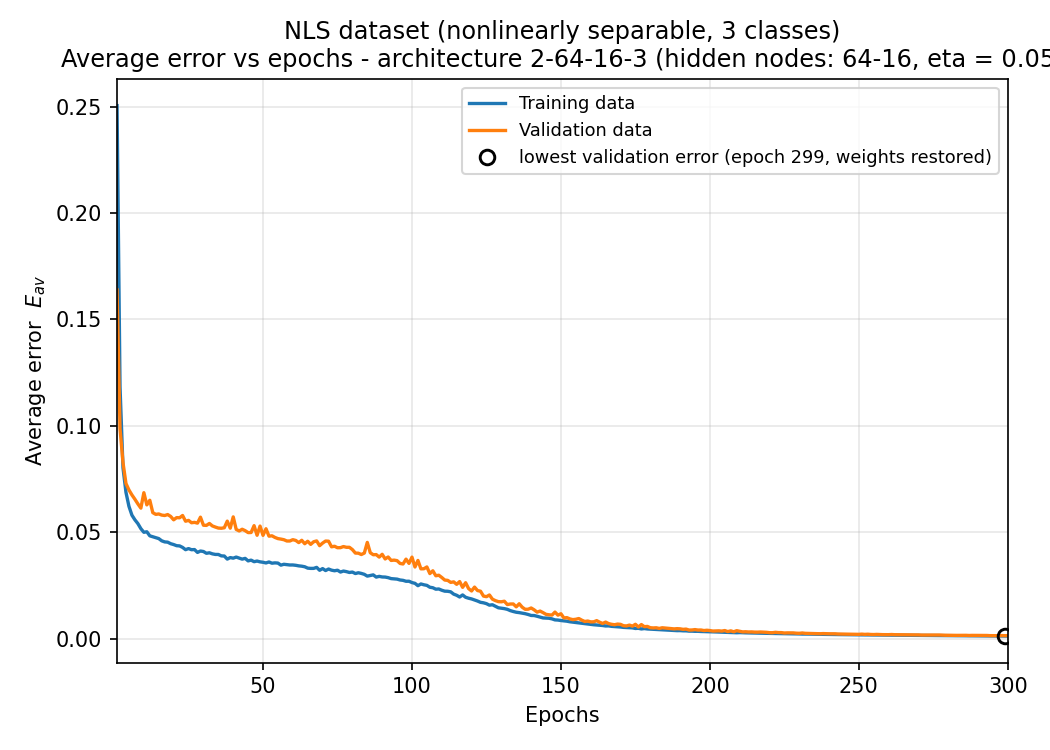
\includegraphics[width=0.78\textwidth,height=7.4cm,keepaspectratio]{figures/classification_nls__error_curves__hidden_64-16.png}
\caption{Average error against epochs, architecture 2-64-16-3 (hidden nodes: 64-16).}
\end{figure}

\begin{figure}[H]
\centering
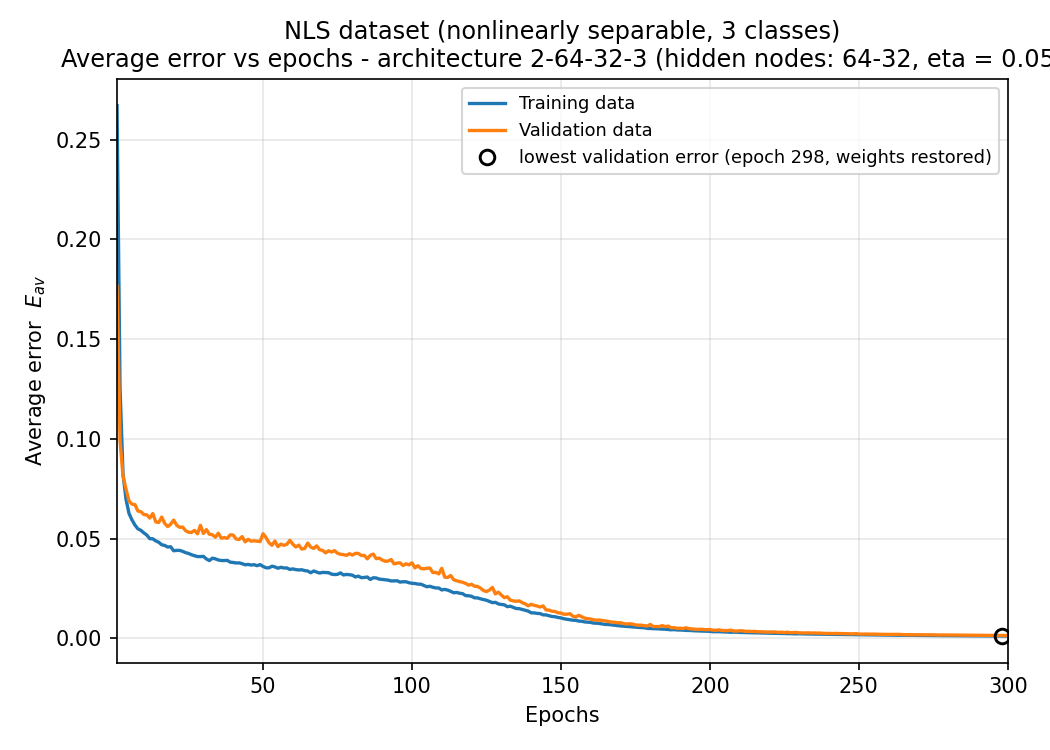
\includegraphics[width=0.78\textwidth,height=7.4cm,keepaspectratio]{figures/classification_nls__error_curves__hidden_64-32.png}
\caption{Average error against epochs, architecture 2-64-32-3 (hidden nodes: 64-32).}
\end{figure}

\clearpage

\subsection{Confusion Matrix and Per-Class Metrics on Validation Data, for Every Architecture}
\noindent\textbf{Architecture 2-16-8-3 (hidden nodes 16-8)} --- classification accuracy = \textbf{100.00\%}

\vspace{2pt}
\noindent
\begin{minipage}[t]{0.42\textwidth}\footnotesize\centering
\begin{tabular}{lrrr}
\toprule
 & \textbf{Pred 1} & \textbf{Pred 2} & \textbf{Pred 3} \\
\midrule
\textbf{True 1} & 100 & 0 & 0 \\
\textbf{True 2} & 0 & 100 & 0 \\
\textbf{True 3} & 0 & 0 & 100 \\
\bottomrule
\end{tabular}
\end{minipage}\hfill
\begin{minipage}[t]{0.56\textwidth}\footnotesize\centering
\begin{tabular}{lrrr}
\toprule
\textbf{Class} & \textbf{Precision} & \textbf{Recall} & \textbf{F-measure} \\
\midrule
1 & 1.0000 & 1.0000 & 1.0000 \\
2 & 1.0000 & 1.0000 & 1.0000 \\
3 & 1.0000 & 1.0000 & 1.0000 \\
\midrule
\textbf{Mean} & 1.0000 & 1.0000 & 1.0000 \\
\bottomrule
\end{tabular}
\end{minipage}

\vspace{8pt}

\noindent\textbf{Architecture 2-32-16-3 (hidden nodes 32-16)} --- classification accuracy = \textbf{100.00\%}

\vspace{2pt}
\noindent
\begin{minipage}[t]{0.42\textwidth}\footnotesize\centering
\begin{tabular}{lrrr}
\toprule
 & \textbf{Pred 1} & \textbf{Pred 2} & \textbf{Pred 3} \\
\midrule
\textbf{True 1} & 100 & 0 & 0 \\
\textbf{True 2} & 0 & 100 & 0 \\
\textbf{True 3} & 0 & 0 & 100 \\
\bottomrule
\end{tabular}
\end{minipage}\hfill
\begin{minipage}[t]{0.56\textwidth}\footnotesize\centering
\begin{tabular}{lrrr}
\toprule
\textbf{Class} & \textbf{Precision} & \textbf{Recall} & \textbf{F-measure} \\
\midrule
1 & 1.0000 & 1.0000 & 1.0000 \\
2 & 1.0000 & 1.0000 & 1.0000 \\
3 & 1.0000 & 1.0000 & 1.0000 \\
\midrule
\textbf{Mean} & 1.0000 & 1.0000 & 1.0000 \\
\bottomrule
\end{tabular}
\end{minipage}

\vspace{8pt}

\noindent\textbf{Architecture 2-64-16-3 (hidden nodes 64-16) (selected)} --- classification accuracy = \textbf{100.00\%}

\vspace{2pt}
\noindent
\begin{minipage}[t]{0.42\textwidth}\footnotesize\centering
\begin{tabular}{lrrr}
\toprule
 & \textbf{Pred 1} & \textbf{Pred 2} & \textbf{Pred 3} \\
\midrule
\textbf{True 1} & 100 & 0 & 0 \\
\textbf{True 2} & 0 & 100 & 0 \\
\textbf{True 3} & 0 & 0 & 100 \\
\bottomrule
\end{tabular}
\end{minipage}\hfill
\begin{minipage}[t]{0.56\textwidth}\footnotesize\centering
\begin{tabular}{lrrr}
\toprule
\textbf{Class} & \textbf{Precision} & \textbf{Recall} & \textbf{F-measure} \\
\midrule
1 & 1.0000 & 1.0000 & 1.0000 \\
2 & 1.0000 & 1.0000 & 1.0000 \\
3 & 1.0000 & 1.0000 & 1.0000 \\
\midrule
\textbf{Mean} & 1.0000 & 1.0000 & 1.0000 \\
\bottomrule
\end{tabular}
\end{minipage}

\vspace{8pt}

\noindent\textbf{Architecture 2-64-32-3 (hidden nodes 64-32)} --- classification accuracy = \textbf{100.00\%}

\vspace{2pt}
\noindent
\begin{minipage}[t]{0.42\textwidth}\footnotesize\centering
\begin{tabular}{lrrr}
\toprule
 & \textbf{Pred 1} & \textbf{Pred 2} & \textbf{Pred 3} \\
\midrule
\textbf{True 1} & 100 & 0 & 0 \\
\textbf{True 2} & 0 & 100 & 0 \\
\textbf{True 3} & 0 & 0 & 100 \\
\bottomrule
\end{tabular}
\end{minipage}\hfill
\begin{minipage}[t]{0.56\textwidth}\footnotesize\centering
\begin{tabular}{lrrr}
\toprule
\textbf{Class} & \textbf{Precision} & \textbf{Recall} & \textbf{F-measure} \\
\midrule
1 & 1.0000 & 1.0000 & 1.0000 \\
2 & 1.0000 & 1.0000 & 1.0000 \\
3 & 1.0000 & 1.0000 & 1.0000 \\
\midrule
\textbf{Mean} & 1.0000 & 1.0000 & 1.0000 \\
\bottomrule
\end{tabular}
\end{minipage}

\vspace{8pt}

\clearpage

\subsection{Best Architecture: 2-64-16-3}
The architecture selected on the validation set is \textbf{2-64-16-3} (hidden nodes: 64-16), trained for 300 epochs. All the plots below are for this model.

\parahead{Average error against epochs.}
\begin{figure}[H]
\centering
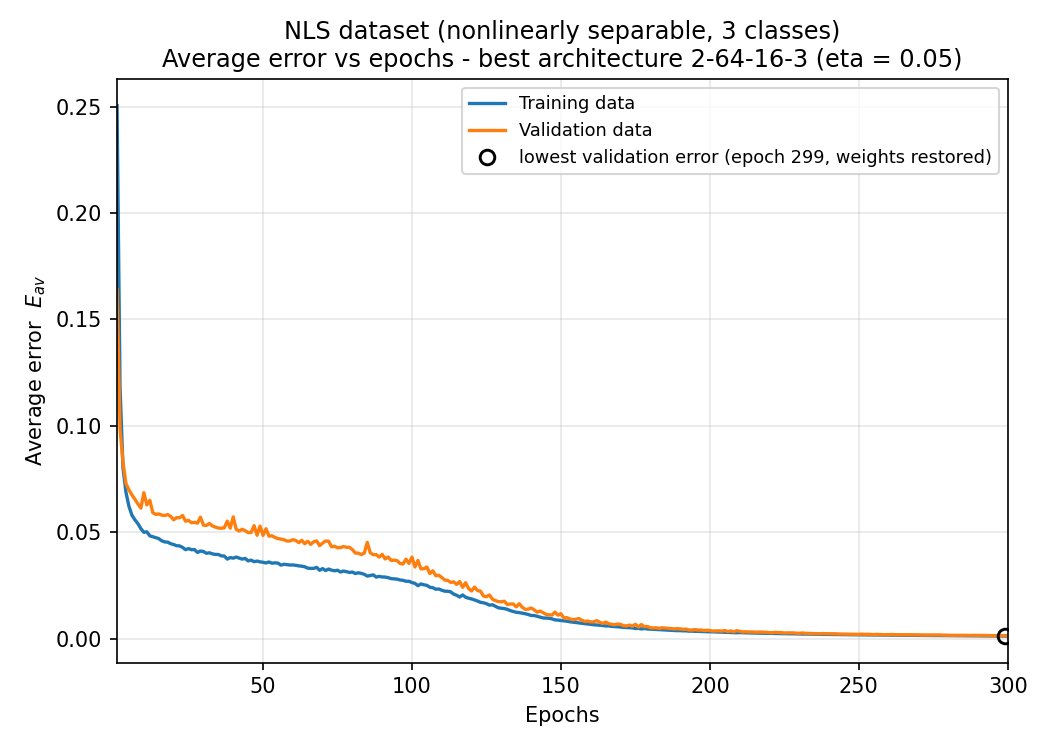
\includegraphics[width=0.8\textwidth,height=8.4cm,keepaspectratio]{figures/classification_nls__best_architecture__error_vs_epochs.png}
\caption{Average error $E_{\mathrm{av}}$ against epochs for the best architecture.}
\end{figure}

\parahead{Decision region superimposed on the training data.}
\begin{figure}[H]
\centering
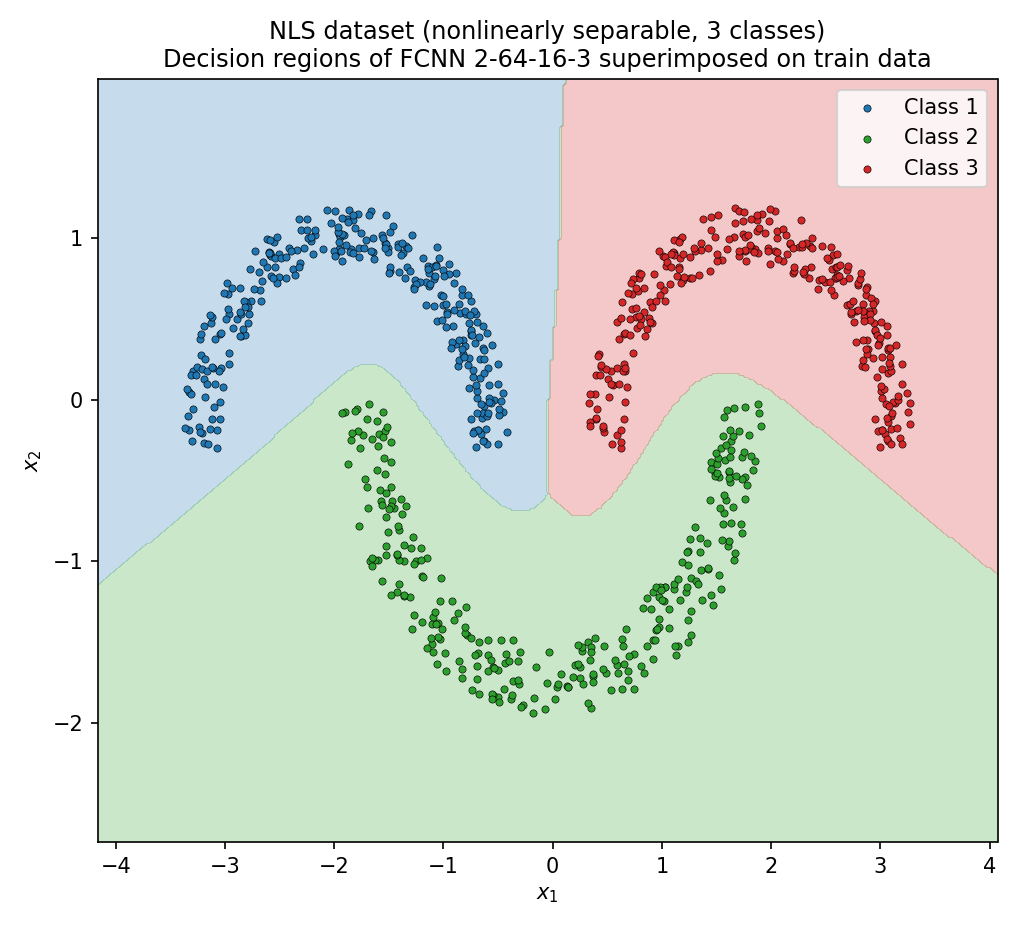
\includegraphics[width=0.82\textwidth,height=10.5cm,keepaspectratio]{figures/classification_nls__best_architecture__decision_region_train.png}
\caption{Decision regions of the best FCNN, superimposed on the training data.}
\end{figure}

\clearpage

\paragraph{Confusion matrix and metrics for the best architecture.}

\noindent\textbf{Training data} --- classification accuracy = \textbf{100.00\%}

\vspace{2pt}
\noindent
\begin{minipage}[t]{0.42\textwidth}\footnotesize\centering
\begin{tabular}{lrrr}
\toprule
 & \textbf{Pred 1} & \textbf{Pred 2} & \textbf{Pred 3} \\
\midrule
\textbf{True 1} & 300 & 0 & 0 \\
\textbf{True 2} & 0 & 300 & 0 \\
\textbf{True 3} & 0 & 0 & 300 \\
\bottomrule
\end{tabular}
\end{minipage}\hfill
\begin{minipage}[t]{0.56\textwidth}\footnotesize\centering
\begin{tabular}{lrrr}
\toprule
\textbf{Class} & \textbf{Precision} & \textbf{Recall} & \textbf{F-measure} \\
\midrule
1 & 1.0000 & 1.0000 & 1.0000 \\
2 & 1.0000 & 1.0000 & 1.0000 \\
3 & 1.0000 & 1.0000 & 1.0000 \\
\midrule
\textbf{Mean} & 1.0000 & 1.0000 & 1.0000 \\
\bottomrule
\end{tabular}
\end{minipage}

\vspace{8pt}

\noindent\textbf{Validation data} --- classification accuracy = \textbf{100.00\%}

\vspace{2pt}
\noindent
\begin{minipage}[t]{0.42\textwidth}\footnotesize\centering
\begin{tabular}{lrrr}
\toprule
 & \textbf{Pred 1} & \textbf{Pred 2} & \textbf{Pred 3} \\
\midrule
\textbf{True 1} & 100 & 0 & 0 \\
\textbf{True 2} & 0 & 100 & 0 \\
\textbf{True 3} & 0 & 0 & 100 \\
\bottomrule
\end{tabular}
\end{minipage}\hfill
\begin{minipage}[t]{0.56\textwidth}\footnotesize\centering
\begin{tabular}{lrrr}
\toprule
\textbf{Class} & \textbf{Precision} & \textbf{Recall} & \textbf{F-measure} \\
\midrule
1 & 1.0000 & 1.0000 & 1.0000 \\
2 & 1.0000 & 1.0000 & 1.0000 \\
3 & 1.0000 & 1.0000 & 1.0000 \\
\midrule
\textbf{Mean} & 1.0000 & 1.0000 & 1.0000 \\
\bottomrule
\end{tabular}
\end{minipage}

\vspace{8pt}

\noindent\textbf{Test data} --- classification accuracy = \textbf{100.00\%}

\vspace{2pt}
\noindent
\begin{minipage}[t]{0.42\textwidth}\footnotesize\centering
\begin{tabular}{lrrr}
\toprule
 & \textbf{Pred 1} & \textbf{Pred 2} & \textbf{Pred 3} \\
\midrule
\textbf{True 1} & 100 & 0 & 0 \\
\textbf{True 2} & 0 & 100 & 0 \\
\textbf{True 3} & 0 & 0 & 100 \\
\bottomrule
\end{tabular}
\end{minipage}\hfill
\begin{minipage}[t]{0.56\textwidth}\footnotesize\centering
\begin{tabular}{lrrr}
\toprule
\textbf{Class} & \textbf{Precision} & \textbf{Recall} & \textbf{F-measure} \\
\midrule
1 & 1.0000 & 1.0000 & 1.0000 \\
2 & 1.0000 & 1.0000 & 1.0000 \\
3 & 1.0000 & 1.0000 & 1.0000 \\
\midrule
\textbf{Mean} & 1.0000 & 1.0000 & 1.0000 \\
\bottomrule
\end{tabular}
\end{minipage}

\vspace{8pt}

\clearpage

\subsection{Outputs of the Hidden Nodes and Output Nodes}
Every hidden node and every output node is plotted in its own figure: the two axes in the base plane are the input variables $x_{1}$ and $x_{2}$ of each example and the vertical axis is the output of that node. The selected network has 83 nodes in total, so the complete set is 249 figures (one per node per split); they are all written to \texttt{outputs/\allowbreak classification\_\allowbreak nls/\allowbreak best\_\allowbreak architecture/\allowbreak node\_\allowbreak outputs/\allowbreak }. The first 6 nodes of each layer are reproduced below for each split.

\parahead{Hidden layer 1 --- train data.}
\begin{figure}[H]
\centering
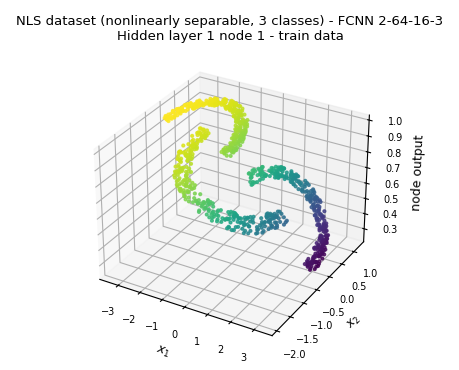
\includegraphics[width=0.323\textwidth]{figures/classification_nls__best_architecture__node_outputs__hidden_layer1__train__node_001.png}\hfill%
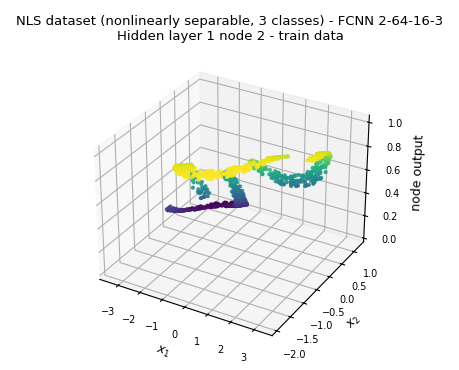
\includegraphics[width=0.323\textwidth]{figures/classification_nls__best_architecture__node_outputs__hidden_layer1__train__node_002.png}\hfill%
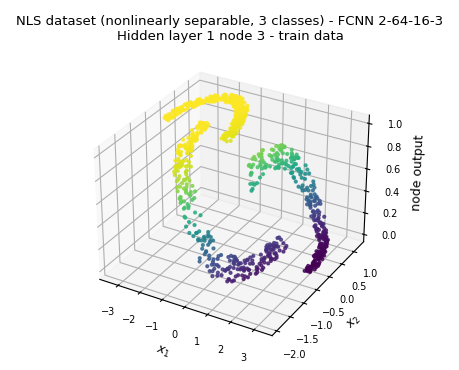
\includegraphics[width=0.323\textwidth]{figures/classification_nls__best_architecture__node_outputs__hidden_layer1__train__node_003.png}\\[4pt]%
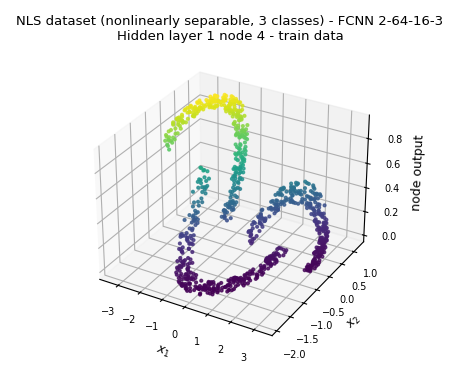
\includegraphics[width=0.323\textwidth]{figures/classification_nls__best_architecture__node_outputs__hidden_layer1__train__node_004.png}\hfill%
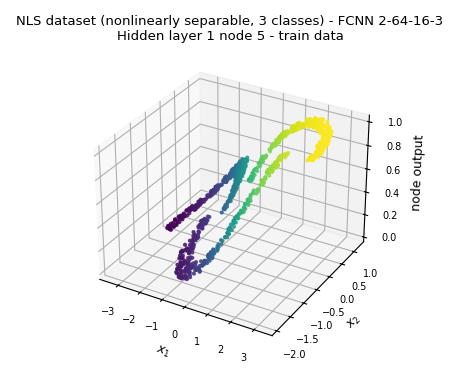
\includegraphics[width=0.323\textwidth]{figures/classification_nls__best_architecture__node_outputs__hidden_layer1__train__node_005.png}\hfill%
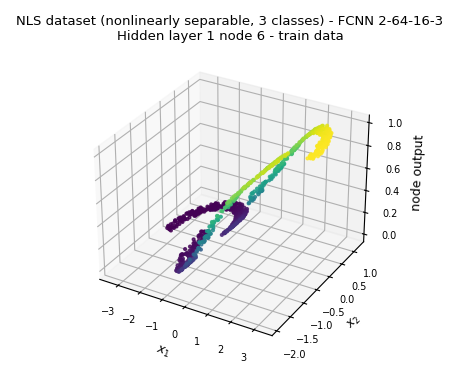
\includegraphics[width=0.323\textwidth]{figures/classification_nls__best_architecture__node_outputs__hidden_layer1__train__node_006.png}
\caption{Outputs of hidden layer 1 nodes 1--6 of 64 (train data). Each node has its own figure; all 64 are in \texttt{outputs/\allowbreak classification\_\allowbreak nls/\allowbreak best\_\allowbreak architecture/\allowbreak node\_\allowbreak outputs/\allowbreak hidden\_\allowbreak layer1/\allowbreak train/\allowbreak }.}
\end{figure}

\parahead{Hidden layer 1 --- val data.}
\begin{figure}[H]
\centering
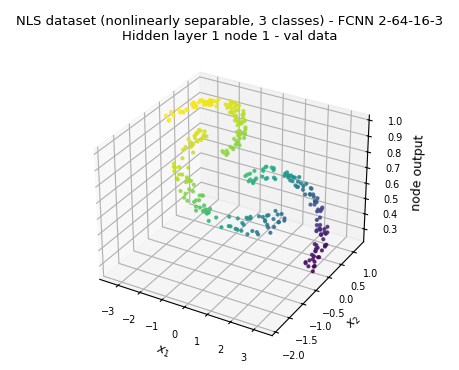
\includegraphics[width=0.323\textwidth]{figures/classification_nls__best_architecture__node_outputs__hidden_layer1__val__node_001.png}\hfill%
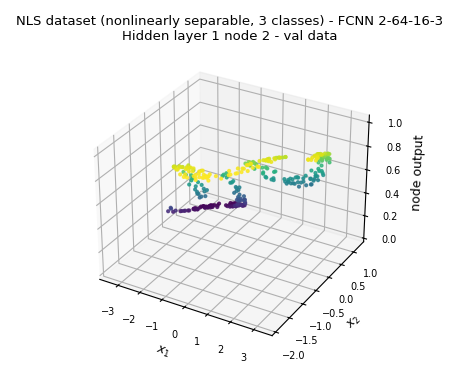
\includegraphics[width=0.323\textwidth]{figures/classification_nls__best_architecture__node_outputs__hidden_layer1__val__node_002.png}\hfill%
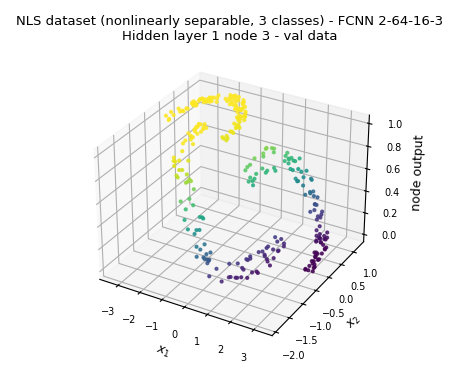
\includegraphics[width=0.323\textwidth]{figures/classification_nls__best_architecture__node_outputs__hidden_layer1__val__node_003.png}\\[4pt]%
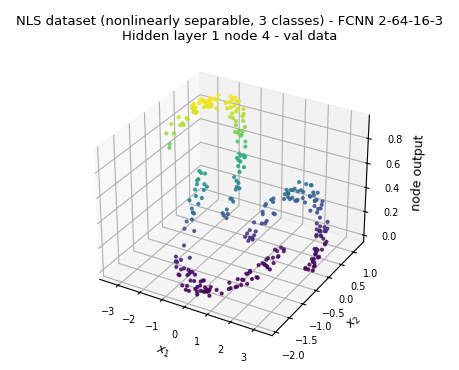
\includegraphics[width=0.323\textwidth]{figures/classification_nls__best_architecture__node_outputs__hidden_layer1__val__node_004.png}\hfill%
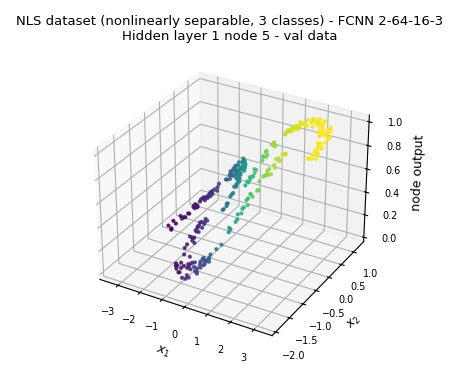
\includegraphics[width=0.323\textwidth]{figures/classification_nls__best_architecture__node_outputs__hidden_layer1__val__node_005.png}\hfill%
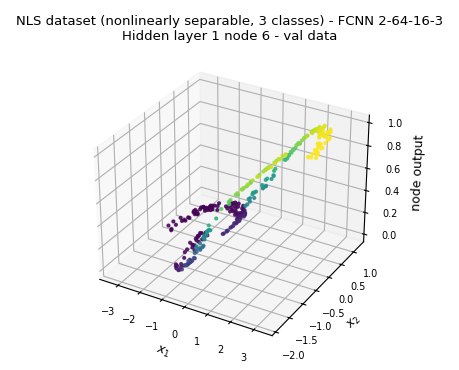
\includegraphics[width=0.323\textwidth]{figures/classification_nls__best_architecture__node_outputs__hidden_layer1__val__node_006.png}
\caption{Outputs of hidden layer 1 nodes 1--6 of 64 (val data). Each node has its own figure; all 64 are in \texttt{outputs/\allowbreak classification\_\allowbreak nls/\allowbreak best\_\allowbreak architecture/\allowbreak node\_\allowbreak outputs/\allowbreak hidden\_\allowbreak layer1/\allowbreak val/\allowbreak }.}
\end{figure}

\parahead{Hidden layer 1 --- test data.}
\begin{figure}[H]
\centering
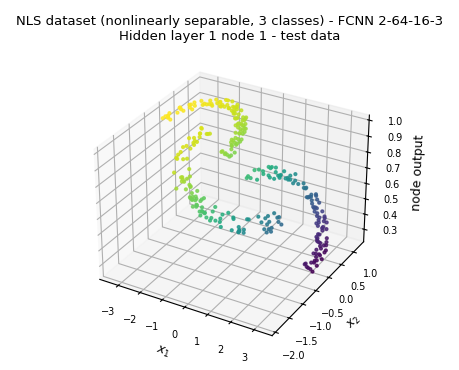
\includegraphics[width=0.323\textwidth]{figures/classification_nls__best_architecture__node_outputs__hidden_layer1__test__node_001.png}\hfill%
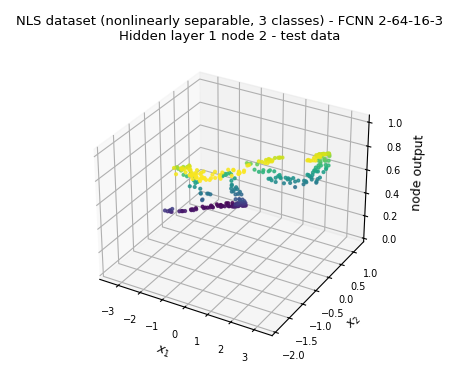
\includegraphics[width=0.323\textwidth]{figures/classification_nls__best_architecture__node_outputs__hidden_layer1__test__node_002.png}\hfill%
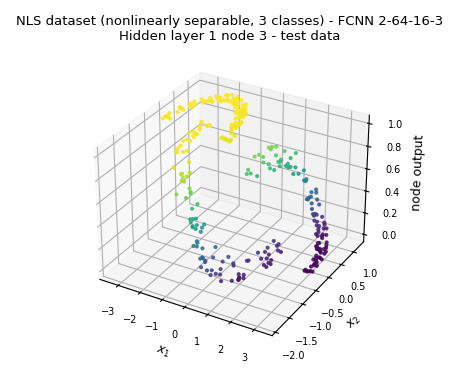
\includegraphics[width=0.323\textwidth]{figures/classification_nls__best_architecture__node_outputs__hidden_layer1__test__node_003.png}\\[4pt]%
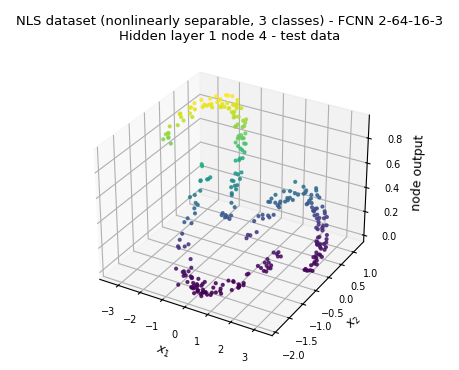
\includegraphics[width=0.323\textwidth]{figures/classification_nls__best_architecture__node_outputs__hidden_layer1__test__node_004.png}\hfill%
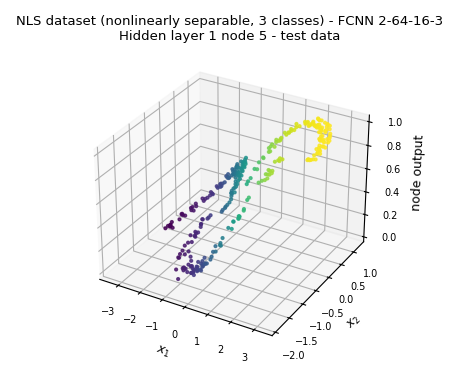
\includegraphics[width=0.323\textwidth]{figures/classification_nls__best_architecture__node_outputs__hidden_layer1__test__node_005.png}\hfill%
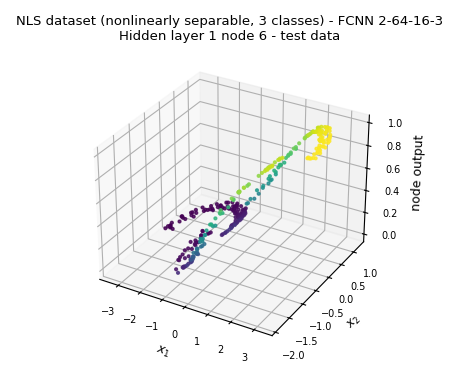
\includegraphics[width=0.323\textwidth]{figures/classification_nls__best_architecture__node_outputs__hidden_layer1__test__node_006.png}
\caption{Outputs of hidden layer 1 nodes 1--6 of 64 (test data). Each node has its own figure; all 64 are in \texttt{outputs/\allowbreak classification\_\allowbreak nls/\allowbreak best\_\allowbreak architecture/\allowbreak node\_\allowbreak outputs/\allowbreak hidden\_\allowbreak layer1/\allowbreak test/\allowbreak }.}
\end{figure}

\clearpage

\parahead{Hidden layer 2 --- train data.}
\begin{figure}[H]
\centering
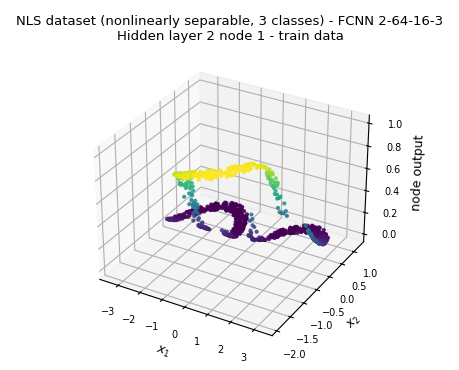
\includegraphics[width=0.323\textwidth]{figures/classification_nls__best_architecture__node_outputs__hidden_layer2__train__node_001.png}\hfill%
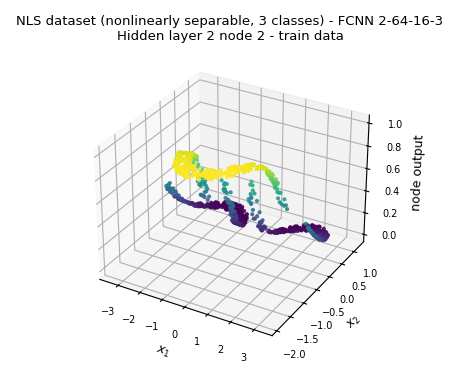
\includegraphics[width=0.323\textwidth]{figures/classification_nls__best_architecture__node_outputs__hidden_layer2__train__node_002.png}\hfill%
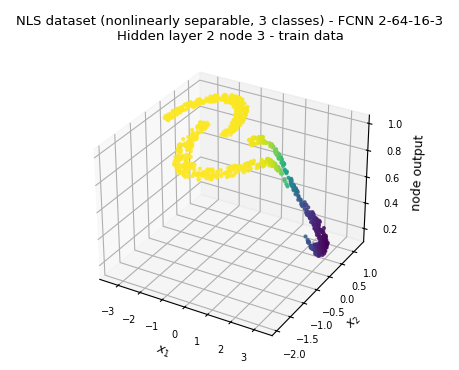
\includegraphics[width=0.323\textwidth]{figures/classification_nls__best_architecture__node_outputs__hidden_layer2__train__node_003.png}\\[4pt]%
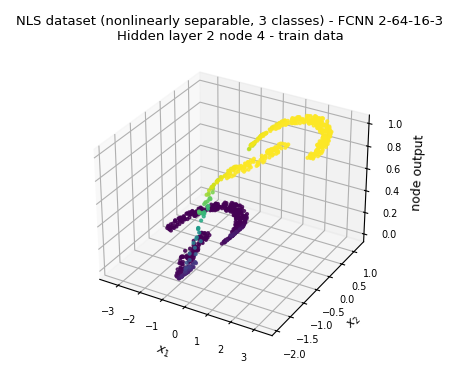
\includegraphics[width=0.323\textwidth]{figures/classification_nls__best_architecture__node_outputs__hidden_layer2__train__node_004.png}\hfill%
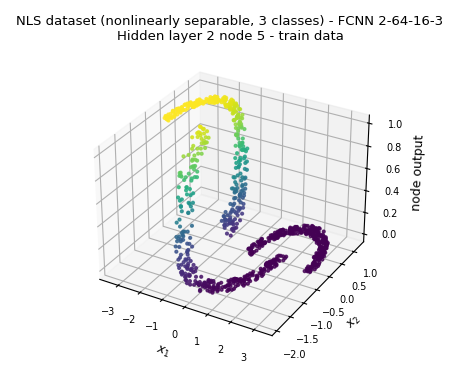
\includegraphics[width=0.323\textwidth]{figures/classification_nls__best_architecture__node_outputs__hidden_layer2__train__node_005.png}\hfill%
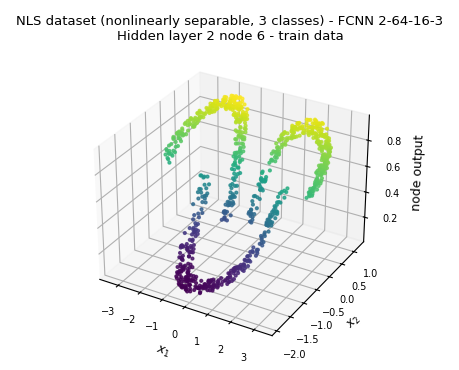
\includegraphics[width=0.323\textwidth]{figures/classification_nls__best_architecture__node_outputs__hidden_layer2__train__node_006.png}
\caption{Outputs of hidden layer 2 nodes 1--6 of 16 (train data). Each node has its own figure; all 16 are in \texttt{outputs/\allowbreak classification\_\allowbreak nls/\allowbreak best\_\allowbreak architecture/\allowbreak node\_\allowbreak outputs/\allowbreak hidden\_\allowbreak layer2/\allowbreak train/\allowbreak }.}
\end{figure}

\parahead{Hidden layer 2 --- val data.}
\begin{figure}[H]
\centering
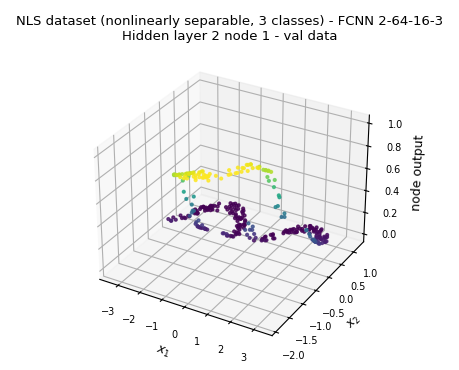
\includegraphics[width=0.323\textwidth]{figures/classification_nls__best_architecture__node_outputs__hidden_layer2__val__node_001.png}\hfill%
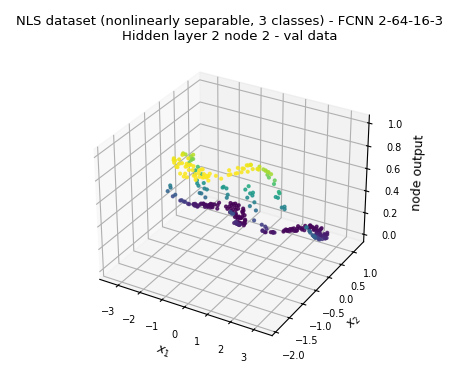
\includegraphics[width=0.323\textwidth]{figures/classification_nls__best_architecture__node_outputs__hidden_layer2__val__node_002.png}\hfill%
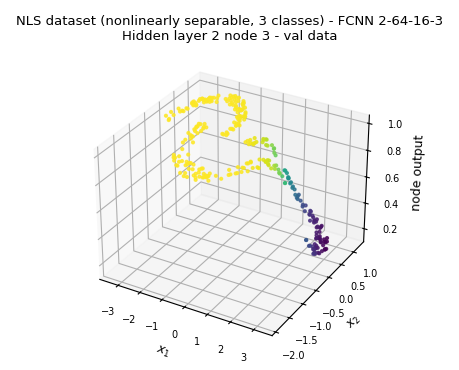
\includegraphics[width=0.323\textwidth]{figures/classification_nls__best_architecture__node_outputs__hidden_layer2__val__node_003.png}\\[4pt]%
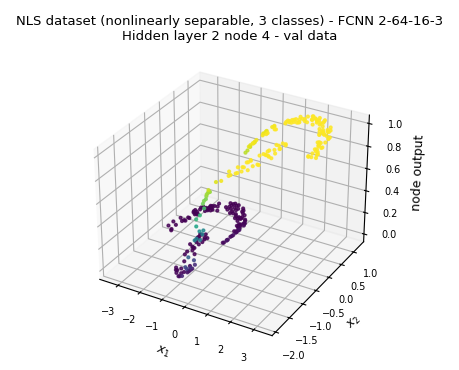
\includegraphics[width=0.323\textwidth]{figures/classification_nls__best_architecture__node_outputs__hidden_layer2__val__node_004.png}\hfill%
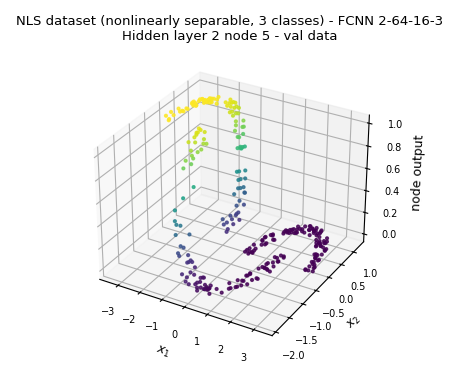
\includegraphics[width=0.323\textwidth]{figures/classification_nls__best_architecture__node_outputs__hidden_layer2__val__node_005.png}\hfill%
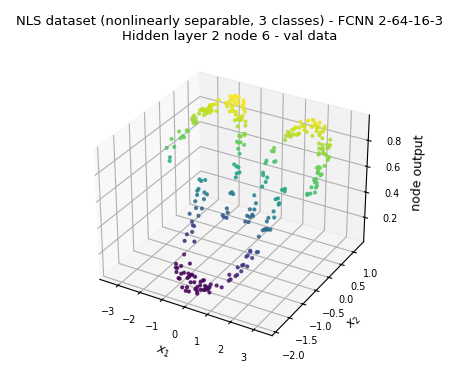
\includegraphics[width=0.323\textwidth]{figures/classification_nls__best_architecture__node_outputs__hidden_layer2__val__node_006.png}
\caption{Outputs of hidden layer 2 nodes 1--6 of 16 (val data). Each node has its own figure; all 16 are in \texttt{outputs/\allowbreak classification\_\allowbreak nls/\allowbreak best\_\allowbreak architecture/\allowbreak node\_\allowbreak outputs/\allowbreak hidden\_\allowbreak layer2/\allowbreak val/\allowbreak }.}
\end{figure}

\parahead{Hidden layer 2 --- test data.}
\begin{figure}[H]
\centering
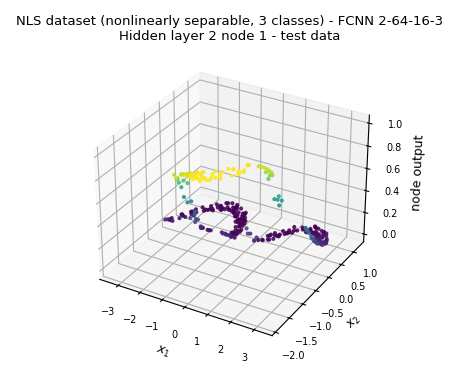
\includegraphics[width=0.323\textwidth]{figures/classification_nls__best_architecture__node_outputs__hidden_layer2__test__node_001.png}\hfill%
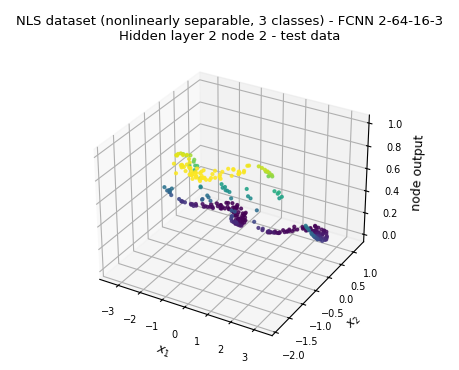
\includegraphics[width=0.323\textwidth]{figures/classification_nls__best_architecture__node_outputs__hidden_layer2__test__node_002.png}\hfill%
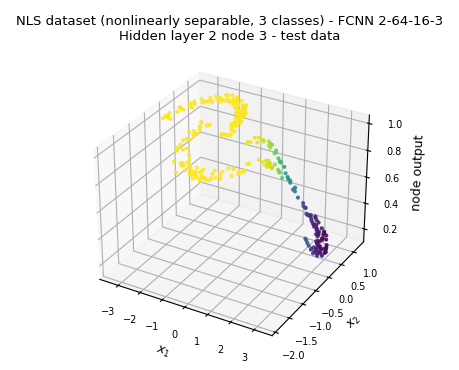
\includegraphics[width=0.323\textwidth]{figures/classification_nls__best_architecture__node_outputs__hidden_layer2__test__node_003.png}\\[4pt]%
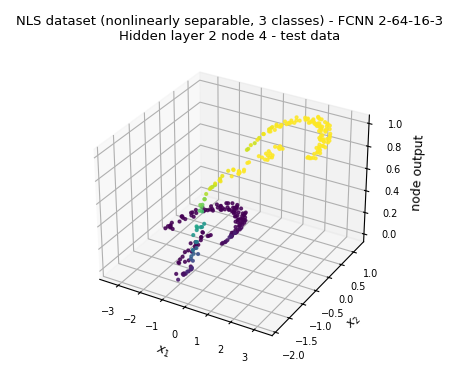
\includegraphics[width=0.323\textwidth]{figures/classification_nls__best_architecture__node_outputs__hidden_layer2__test__node_004.png}\hfill%
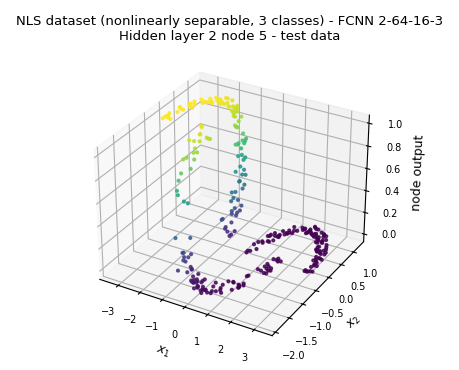
\includegraphics[width=0.323\textwidth]{figures/classification_nls__best_architecture__node_outputs__hidden_layer2__test__node_005.png}\hfill%
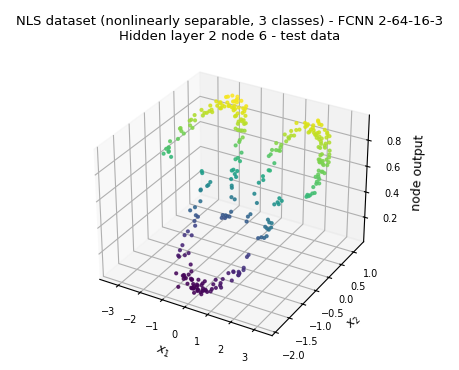
\includegraphics[width=0.323\textwidth]{figures/classification_nls__best_architecture__node_outputs__hidden_layer2__test__node_006.png}
\caption{Outputs of hidden layer 2 nodes 1--6 of 16 (test data). Each node has its own figure; all 16 are in \texttt{outputs/\allowbreak classification\_\allowbreak nls/\allowbreak best\_\allowbreak architecture/\allowbreak node\_\allowbreak outputs/\allowbreak hidden\_\allowbreak layer2/\allowbreak test/\allowbreak }.}
\end{figure}

\clearpage

\parahead{Output layer --- train data.}
\begin{figure}[H]
\centering
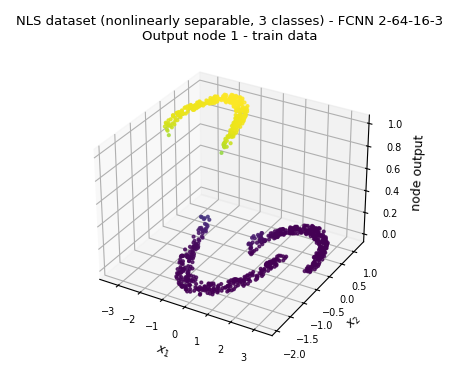
\includegraphics[width=0.323\textwidth]{figures/classification_nls__best_architecture__node_outputs__output_layer__train__node_001.png}\hfill%
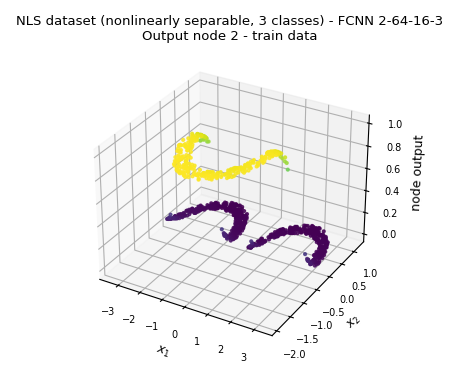
\includegraphics[width=0.323\textwidth]{figures/classification_nls__best_architecture__node_outputs__output_layer__train__node_002.png}\hfill%
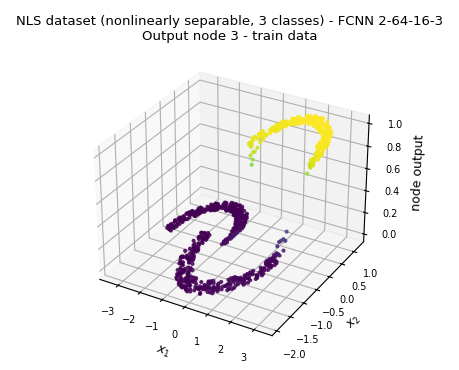
\includegraphics[width=0.323\textwidth]{figures/classification_nls__best_architecture__node_outputs__output_layer__train__node_003.png}
\caption{Outputs of all 3 output nodes (train data), one figure per node.}
\end{figure}

\parahead{Output layer --- val data.}
\begin{figure}[H]
\centering
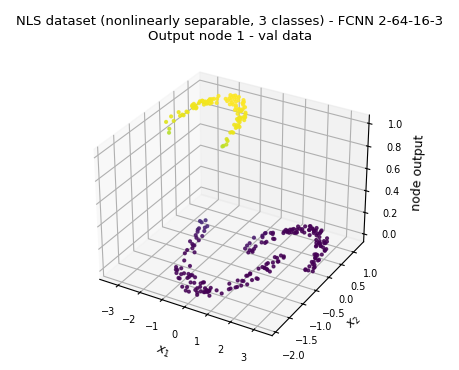
\includegraphics[width=0.323\textwidth]{figures/classification_nls__best_architecture__node_outputs__output_layer__val__node_001.png}\hfill%
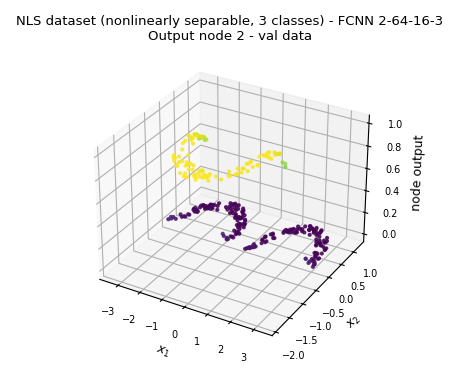
\includegraphics[width=0.323\textwidth]{figures/classification_nls__best_architecture__node_outputs__output_layer__val__node_002.png}\hfill%
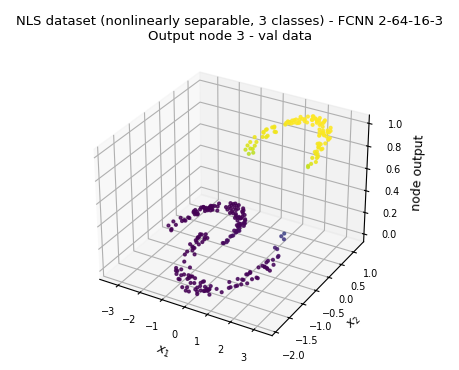
\includegraphics[width=0.323\textwidth]{figures/classification_nls__best_architecture__node_outputs__output_layer__val__node_003.png}
\caption{Outputs of all 3 output nodes (val data), one figure per node.}
\end{figure}

\parahead{Output layer --- test data.}
\begin{figure}[H]
\centering
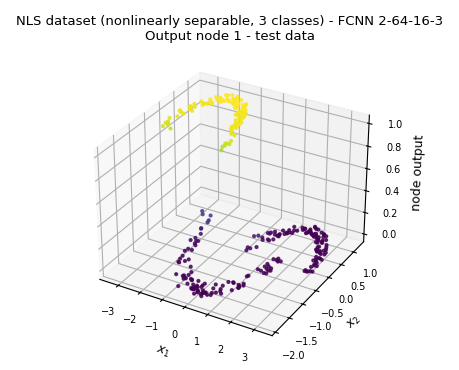
\includegraphics[width=0.323\textwidth]{figures/classification_nls__best_architecture__node_outputs__output_layer__test__node_001.png}\hfill%
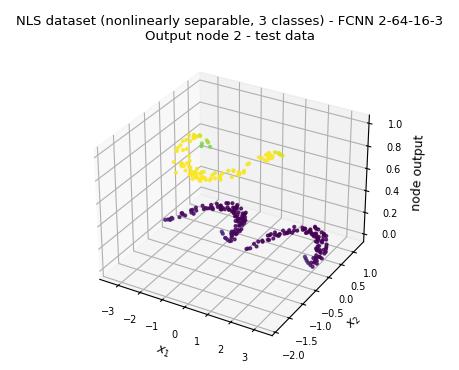
\includegraphics[width=0.323\textwidth]{figures/classification_nls__best_architecture__node_outputs__output_layer__test__node_002.png}\hfill%
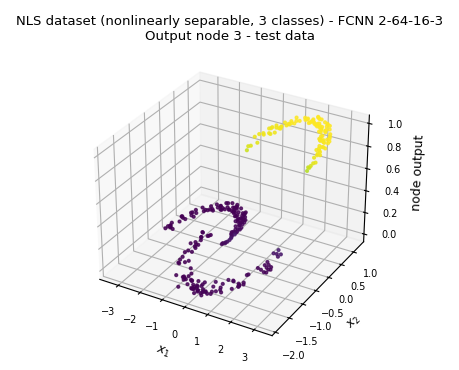
\includegraphics[width=0.323\textwidth]{figures/classification_nls__best_architecture__node_outputs__output_layer__test__node_003.png}
\caption{Outputs of all 3 output nodes (test data), one figure per node.}
\end{figure}

\clearpage

\subsection{Comparison with the Single-Neuron Model (Assignment-1)}
The Assignment-1 model --- one perceptron per pair of classes, combined by one-against-one majority voting --- was retrained on exactly the same 60/20/20 split and scored with the same from-scratch metric code, so the two rows below are directly comparable.

\begin{table}[H]
\centering
\caption{FCNN against the Assignment-1 single-neuron model.}
\setlength{\tabcolsep}{4pt}
\footnotesize
\resizebox{\textwidth}{!}{%
\begin{tabular}{lrrrrr}
\toprule
\textbf{Model} & \textbf{Val acc.\%} & \textbf{Test acc.\%} & \textbf{Test mean prec.} & \textbf{Test mean recall} & \textbf{Test mean $F$} \\
\midrule
Single neuron (one-against-one perceptron) & 91.67 & 92.67 & 0.9263 & 0.9267 & 0.9264 \\
\rowcolor{bestrow} \textbf{FCNN 2-64-16-3 (Assignment-2)} & \textbf{100.00} & \textbf{100.00} & \textbf{1.0000} & \textbf{1.0000} & \textbf{1.0000} \\
\bottomrule
\end{tabular}
}
\end{table}

\begin{figure}[H]
\centering
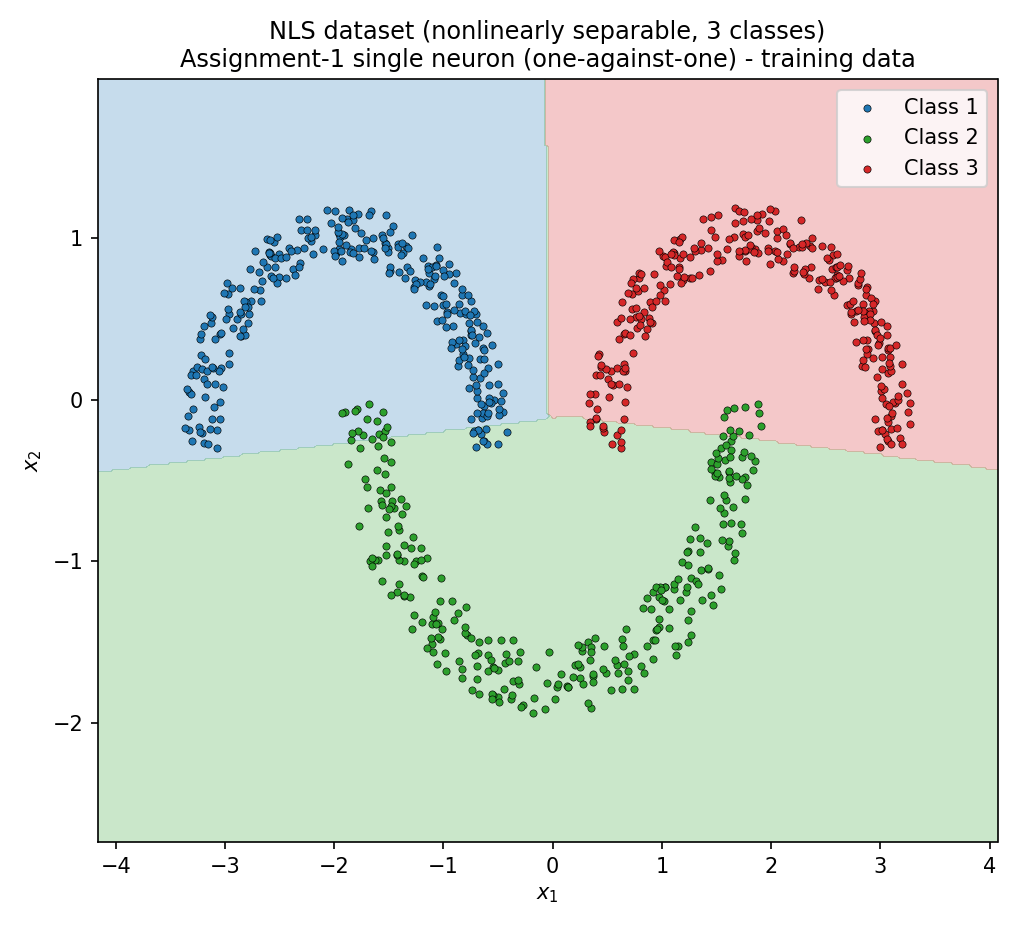
\includegraphics[width=0.8\textwidth,height=9.6cm,keepaspectratio]{figures/classification_nls__baseline_single_neuron_decision_region_train.png}
\caption{Decision regions of the Assignment-1 single-neuron model on the same training data.}
\end{figure}

\subsection{Inferences}
\begin{itemize}
  \item The NLS classes are interleaved arcs, so the class boundaries are strongly nonlinear. The best two-hidden-layer network, 2-64-16-3, reaches 100.00\% on validation and 100.00\% on test data.
  \item This is where the FCNN clearly beats the single neuron: the Assignment-1 one-against-one perceptron reaches only 92.67\% on the same test data, i.e. the FCNN gains +7.33 percentage points. The per-class F-measure improves from 0.9264 to 1.0000.
  \item The reason is visible in the two decision-region plots: the single neuron can only draw straight lines, so it necessarily cuts through the arcs and misclassifies the points near the concave parts of the boundary, whereas the FCNN wraps its boundary around the arcs.
  \item All 4 architectures reach 100.00\% validation accuracy, so two hidden layers of even modest width are already sufficient for this dataset; the extra nodes in the larger networks add parameters without adding accuracy.
  \item The hidden-layer output plots make the mechanism explicit: the first hidden layer produces oriented sigmoid ridges (soft half-planes), and the second hidden layer combines them into localised bump-like surfaces that follow the arcs. The output nodes are then close to 1 over one arc and close to 0 elsewhere.
  \item The average-error curve of the best architecture falls steeply during the first epochs and then flattens; training ran for 300 epochs before the convergence criterion stopped it. Training and validation curves stay close together, so there is no sign of overfitting at this network size.
  \item Training, validation and test metrics of the selected model agree closely, which is what one expects when the model is selected on data that is disjoint from the test set and the three splits are drawn from the same distribution.
\end{itemize}

\clearpage

\section{Regression --- Dataset 1 (Univariate, 1-D Input)}
Model: an FCNN with one hidden layer, logistic hidden nodes and a single linear output node, trained by SGD backpropagation with the squared-error loss and learning rate $\eta = 0.01$. 4 architectures were trained and compared on the validation set.

\subsection{RMSE and \%RMSE for the Different Architectures}
\begin{table}[H]
\centering
\caption{RMSE and \%RMSE on training and validation data for every architecture. The selected architecture is highlighted.}
\setlength{\tabcolsep}{4pt}
\footnotesize
\resizebox{\textwidth}{!}{%
\begin{tabular}{llrrrrrrr}
\toprule
\textbf{Hidden nodes} & \textbf{Architecture} & \textbf{Hidden layers} & \textbf{Params} & \textbf{Epochs} & \textbf{RMSE (train)} & \textbf{\%RMSE (train)} & \textbf{RMSE (val)} & \textbf{\%RMSE (val)} \\
\midrule
\rowcolor{bestrow} \textbf{8} & \textbf{1-8-1} & \textbf{1} & \textbf{25} & \textbf{250} & \textbf{0.0590} & \textbf{2.314} & \textbf{0.0625} & \textbf{2.646} \\
16 & 1-16-1 & 1 & 49 & 300 & 0.0635 & 2.489 & 0.0663 & 2.806 \\
32 & 1-32-1 & 1 & 97 & 300 & 0.0667 & 2.613 & 0.0684 & 2.897 \\
64 & 1-64-1 & 1 & 193 & 300 & 0.0685 & 2.684 & 0.0703 & 2.978 \\
\bottomrule
\end{tabular}
}
\end{table}

\subsection{Best Architecture: 1-8-1}
\begin{table}[H]
\centering
\caption{RMSE and \%RMSE of the selected architecture 1-8-1 on training, validation and test data.}
\setlength{\tabcolsep}{4pt}
\footnotesize
\begin{tabular}{lrr}
\toprule
\textbf{Data} & \textbf{RMSE} & \textbf{\%RMSE} \\
\midrule
Train & 0.0590 & 2.3136 \\
Val & 0.0625 & 2.6461 \\
Test & 0.0590 & 2.3726 \\
\bottomrule
\end{tabular}
\end{table}

\begin{figure}[H]
\centering
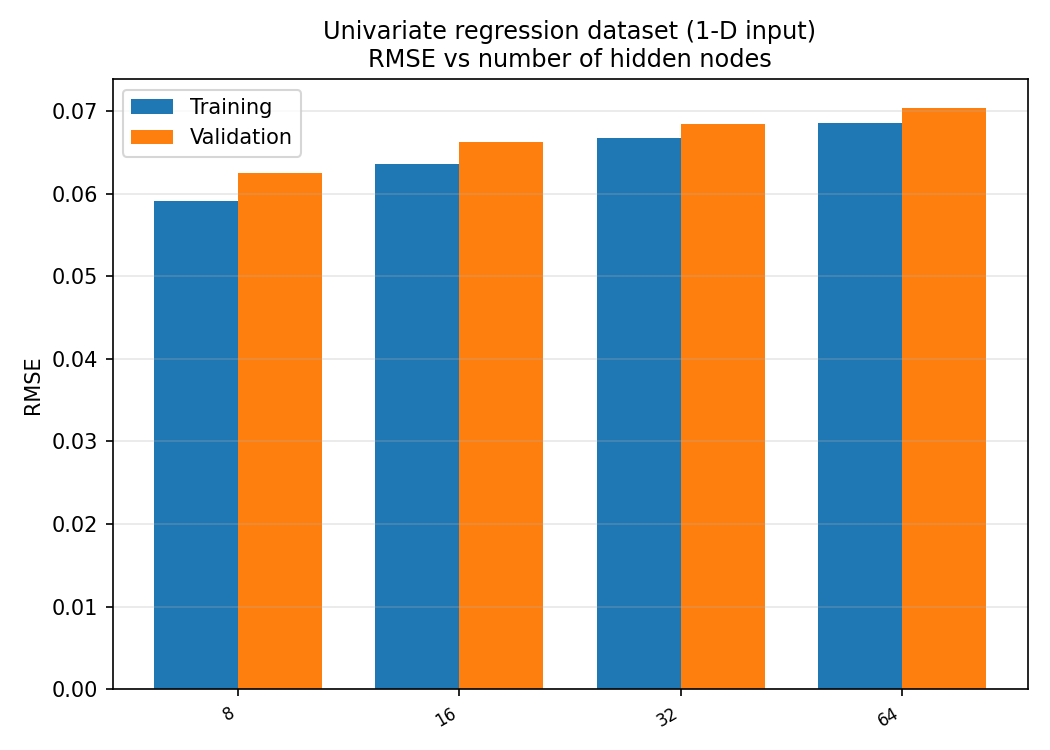
\includegraphics[width=0.78\textwidth,height=7.6cm,keepaspectratio]{figures/regression_univariate__model_selection_rmse.png}
\caption{RMSE against the number of hidden nodes.}
\end{figure}

Average error against epochs for each architecture that was tried, one graph per architecture. They are deliberately not overlaid on a single axis: with several architectures the curves sit on top of one another and none of them can be read.

\begin{figure}[H]
\centering
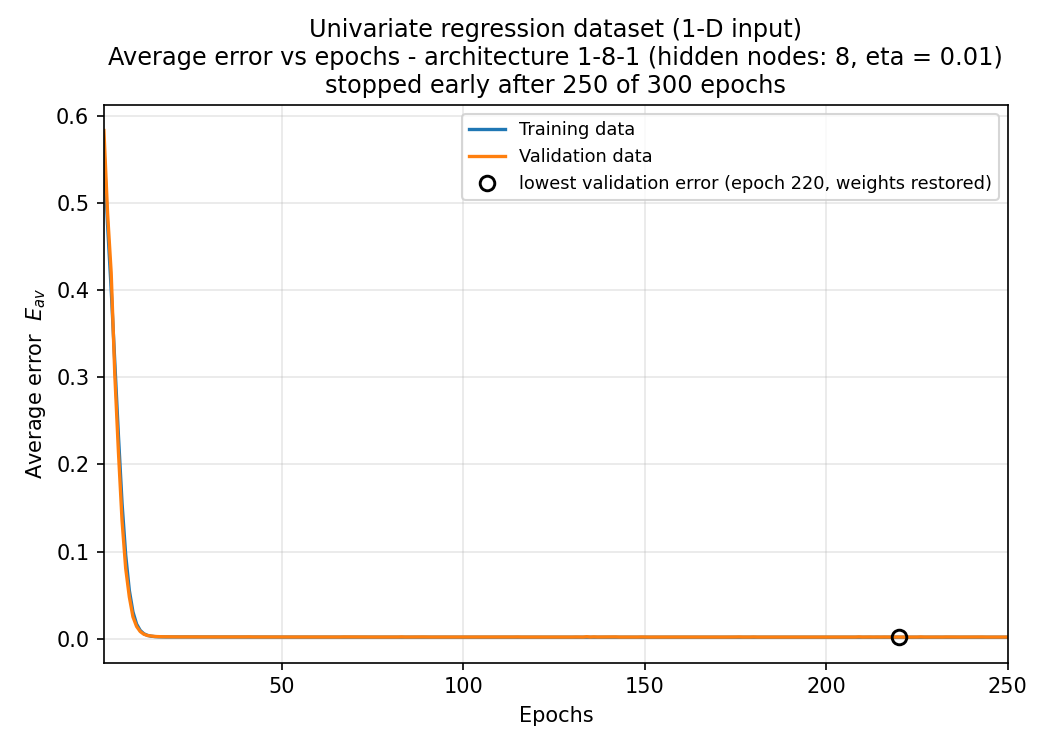
\includegraphics[width=0.78\textwidth,height=7.4cm,keepaspectratio]{figures/regression_univariate__error_curves__hidden_8.png}
\caption{Average error against epochs, architecture 1-8-1 (hidden nodes: 8).}
\end{figure}

\begin{figure}[H]
\centering
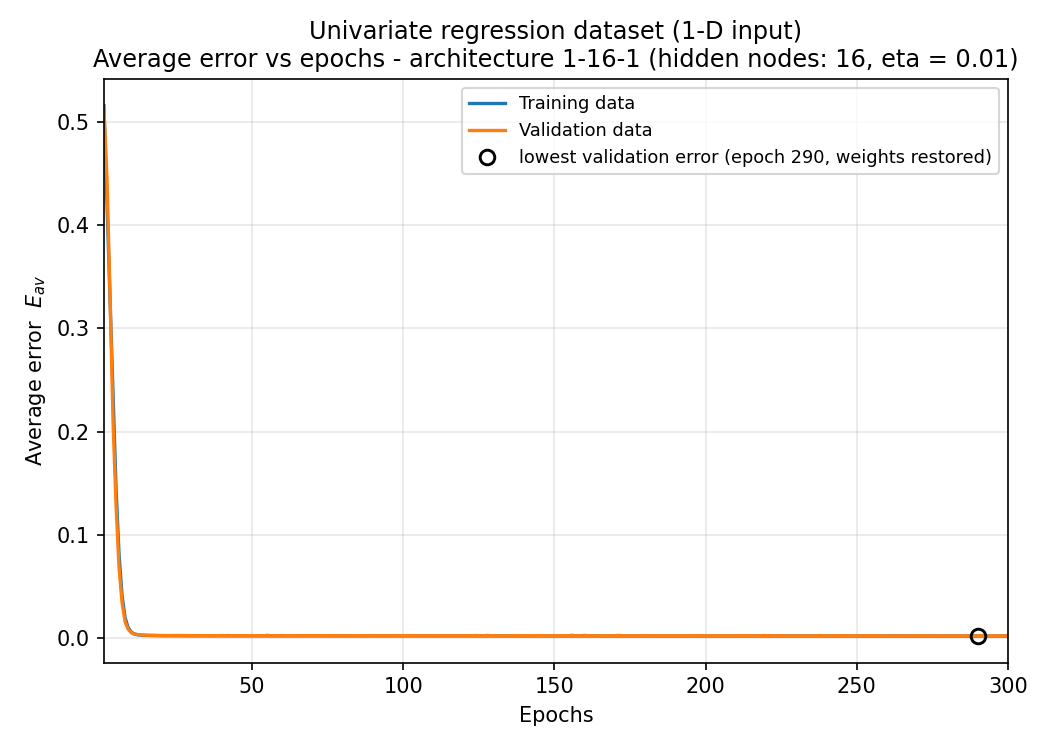
\includegraphics[width=0.78\textwidth,height=7.4cm,keepaspectratio]{figures/regression_univariate__error_curves__hidden_16.png}
\caption{Average error against epochs, architecture 1-16-1 (hidden nodes: 16).}
\end{figure}

\begin{figure}[H]
\centering
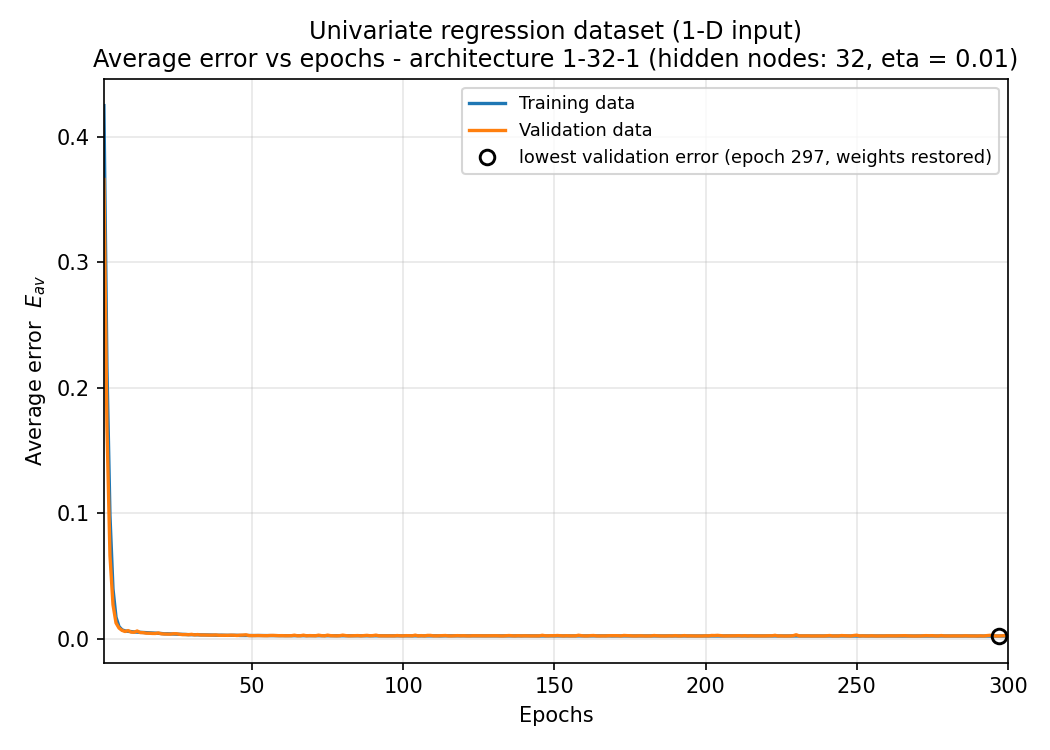
\includegraphics[width=0.78\textwidth,height=7.4cm,keepaspectratio]{figures/regression_univariate__error_curves__hidden_32.png}
\caption{Average error against epochs, architecture 1-32-1 (hidden nodes: 32).}
\end{figure}

\begin{figure}[H]
\centering
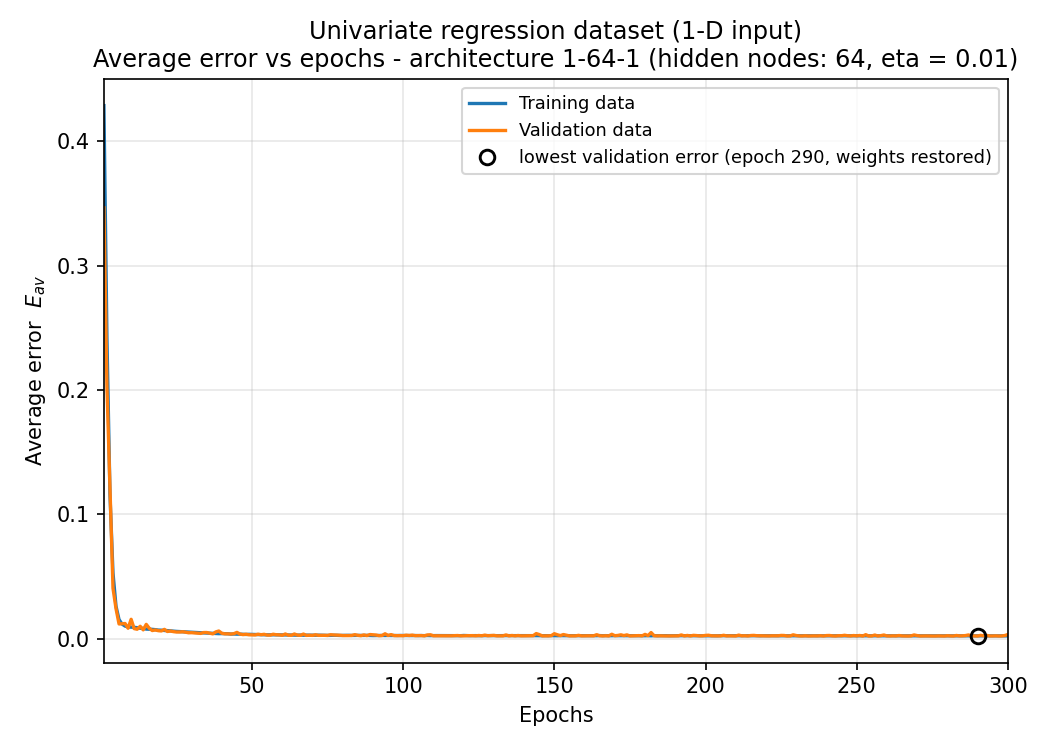
\includegraphics[width=0.78\textwidth,height=7.4cm,keepaspectratio]{figures/regression_univariate__error_curves__hidden_64.png}
\caption{Average error against epochs, architecture 1-64-1 (hidden nodes: 64).}
\end{figure}

\clearpage

\parahead{Average error against epochs (best architecture).}
\begin{figure}[H]
\centering
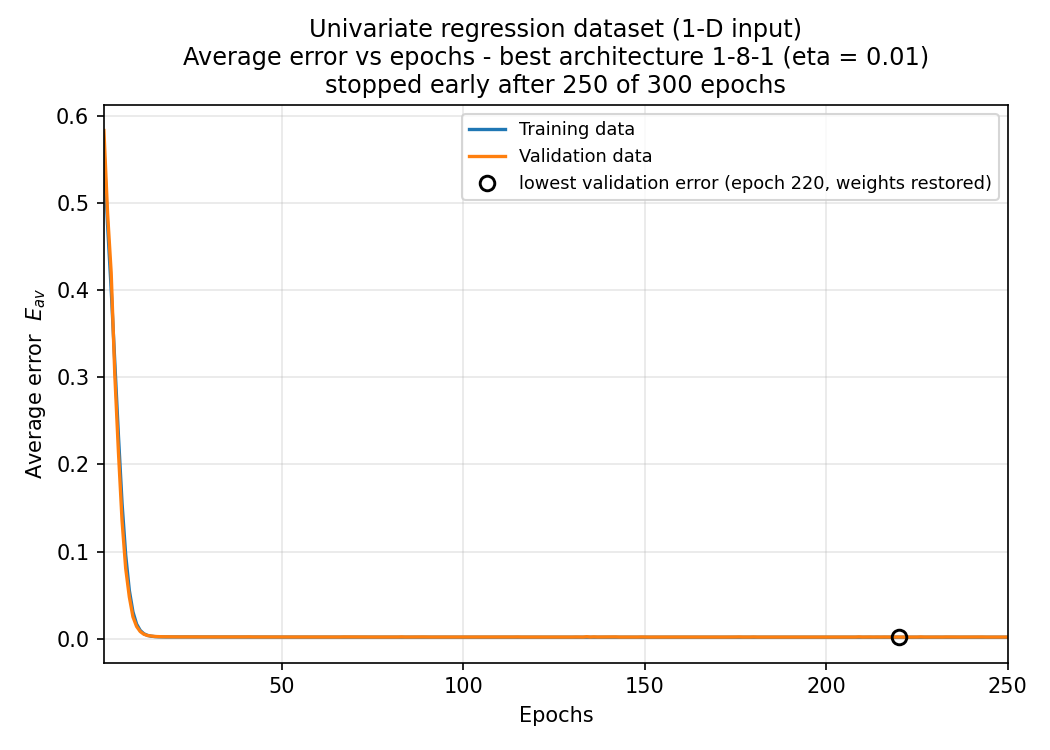
\includegraphics[width=0.8\textwidth,height=8.4cm,keepaspectratio]{figures/regression_univariate__best_architecture__error_vs_epochs.png}
\caption{Average error $E_{\mathrm{av}}$ against epochs for the best architecture.}
\end{figure}

\subsection{Model Output Superimposed on the Target Output}
In the plots below the $x$-axis is the input $x$ and the $y$-axis is the target / model output.

\begin{figure}[H]
\centering
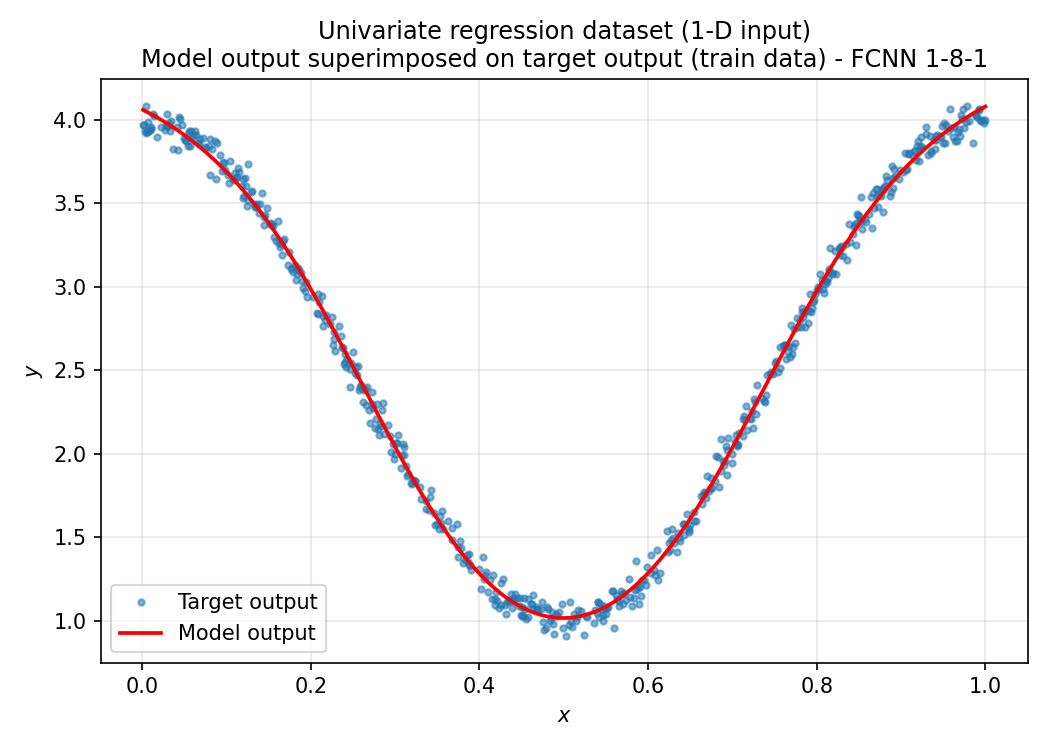
\includegraphics[width=0.8\textwidth,height=9.2cm,keepaspectratio]{figures/regression_univariate__best_architecture__model_vs_target_train.png}
\caption{Model output superimposed on the target output (train data).}
\end{figure}

\begin{figure}[H]
\centering
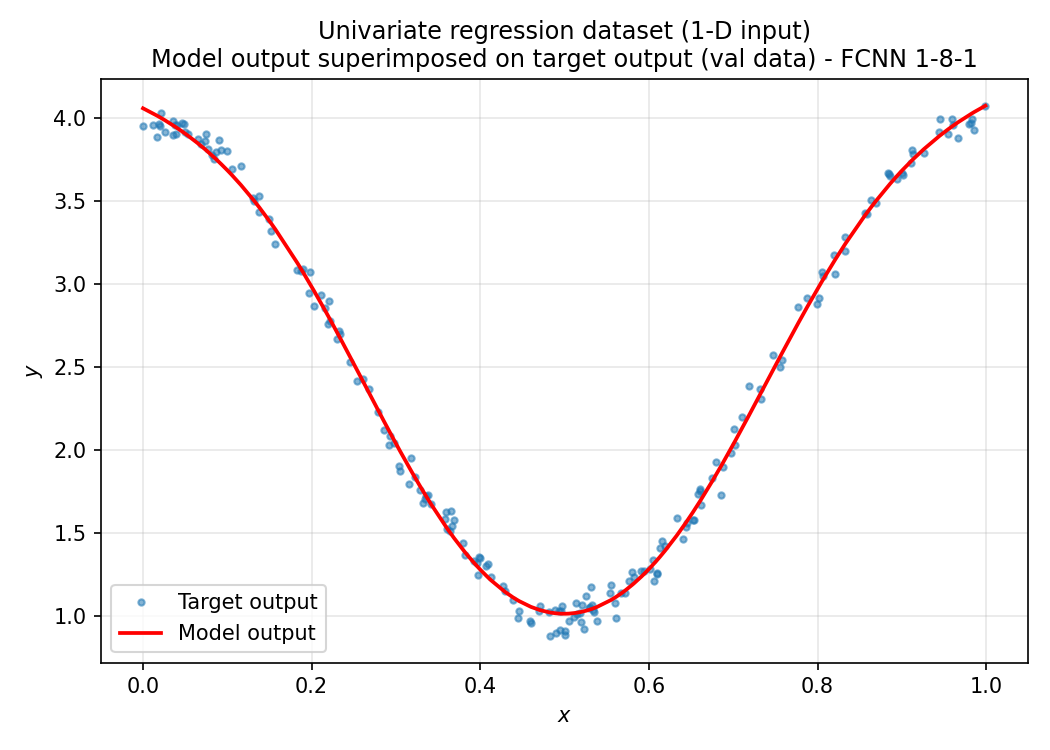
\includegraphics[width=0.8\textwidth,height=9.2cm,keepaspectratio]{figures/regression_univariate__best_architecture__model_vs_target_val.png}
\caption{Model output superimposed on the target output (val data).}
\end{figure}

\begin{figure}[H]
\centering
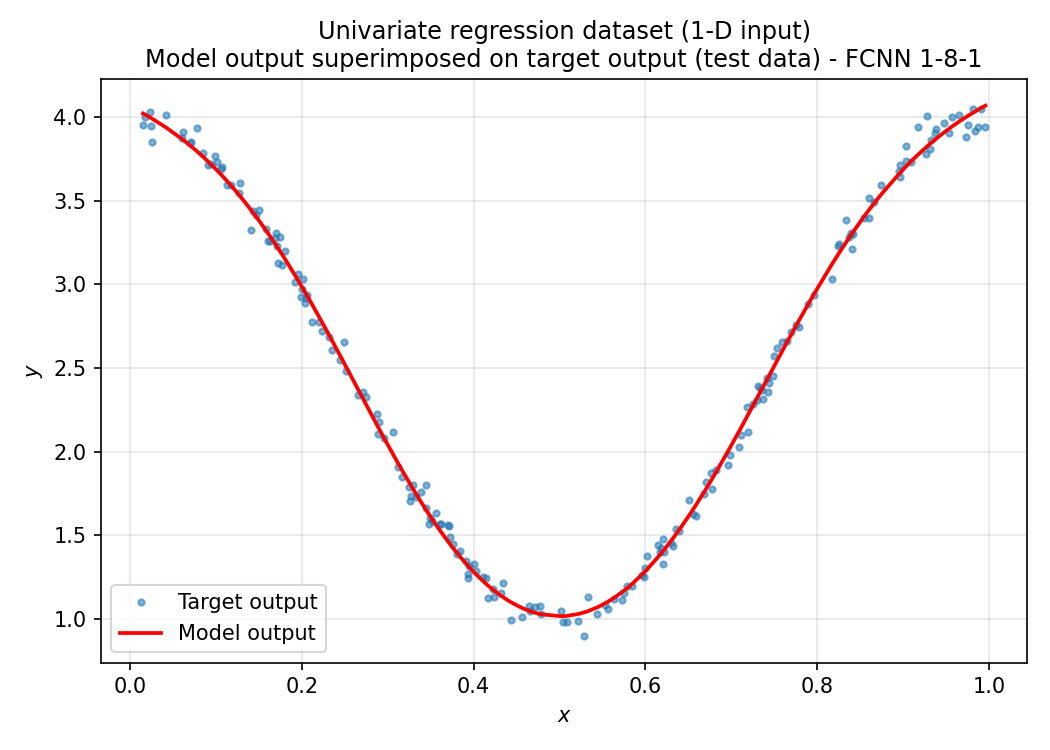
\includegraphics[width=0.8\textwidth,height=9.2cm,keepaspectratio]{figures/regression_univariate__best_architecture__model_vs_target_test.png}
\caption{Model output superimposed on the target output (test data).}
\end{figure}

\clearpage

\subsection{Scatter Plot of Target Output against Model Output}
\begin{figure}[H]
\centering
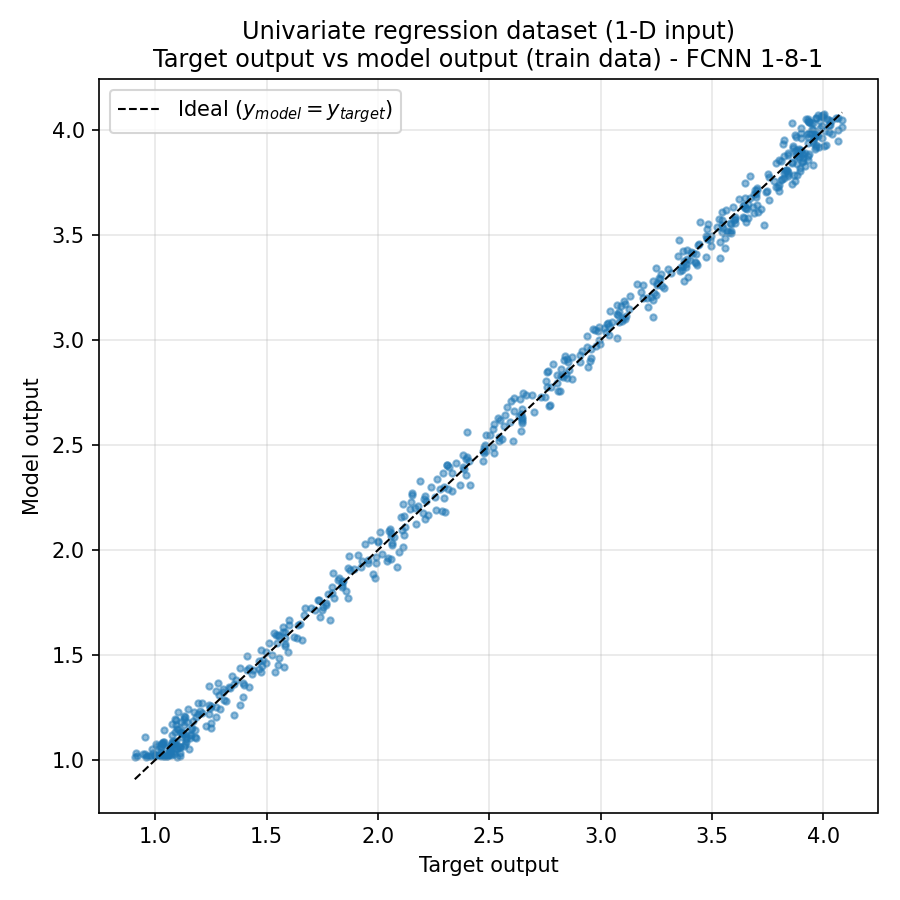
\includegraphics[width=0.66\textwidth,height=8.0cm,keepaspectratio]{figures/regression_univariate__best_architecture__scatter_target_vs_model_train.png}
\caption{Target output (horizontal axis) against model output (vertical axis), train data.}
\end{figure}

\begin{figure}[H]
\centering
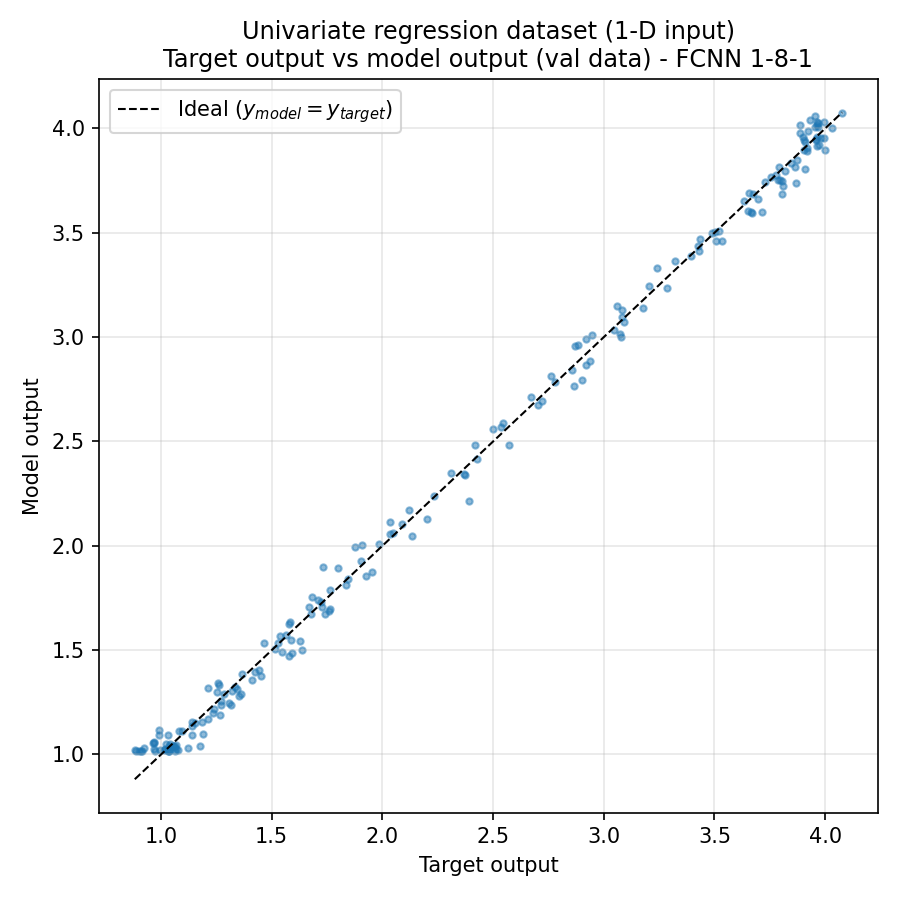
\includegraphics[width=0.66\textwidth,height=8.0cm,keepaspectratio]{figures/regression_univariate__best_architecture__scatter_target_vs_model_val.png}
\caption{Target output (horizontal axis) against model output (vertical axis), val data.}
\end{figure}

\begin{figure}[H]
\centering
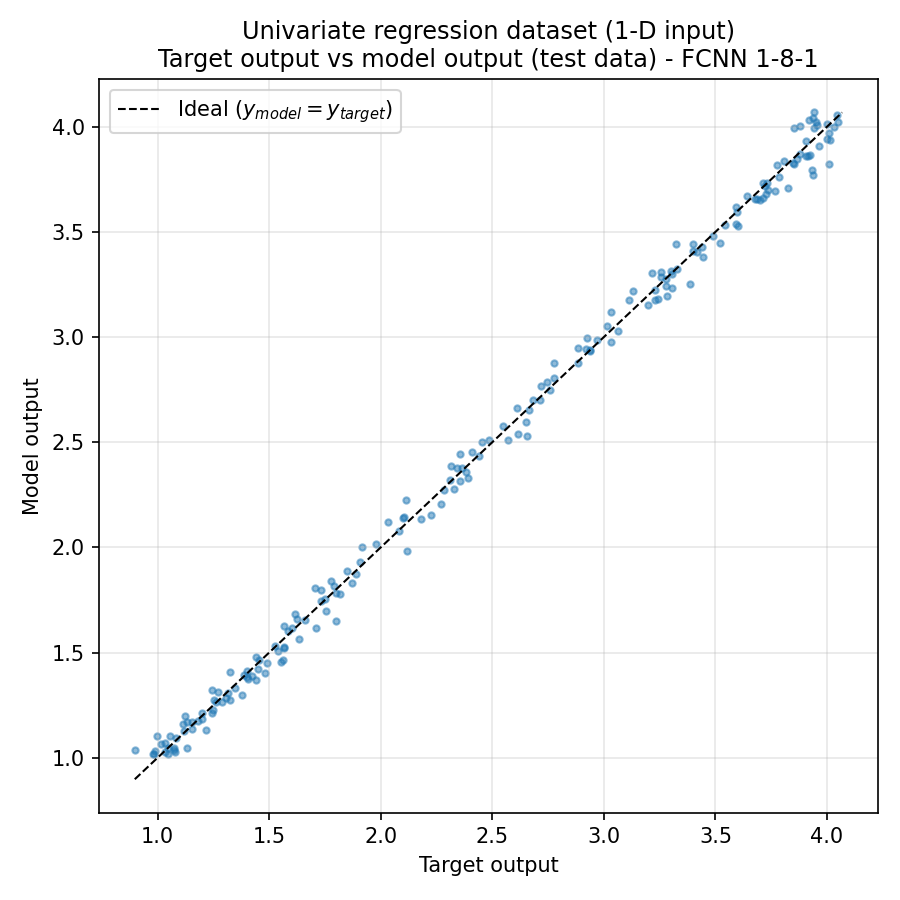
\includegraphics[width=0.66\textwidth,height=8.0cm,keepaspectratio]{figures/regression_univariate__best_architecture__scatter_target_vs_model_test.png}
\caption{Target output (horizontal axis) against model output (vertical axis), test data.}
\end{figure}

\clearpage

\subsection{Outputs of the Hidden Nodes and Output Node}
Every hidden node and the output node is plotted in its own figure: the vertical axis is the output of that node and the remaining axes are the input variables of each example. The selected network has 9 nodes in total, so the complete set is 27 figures (one per node per split); they are all written to \texttt{outputs/\allowbreak regression\_\allowbreak univariate/\allowbreak best\_\allowbreak architecture/\allowbreak node\_\allowbreak outputs/\allowbreak }. The first 6 nodes of each layer are reproduced below for each split.

\parahead{Hidden layer 1 --- train data.}
\begin{figure}[H]
\centering
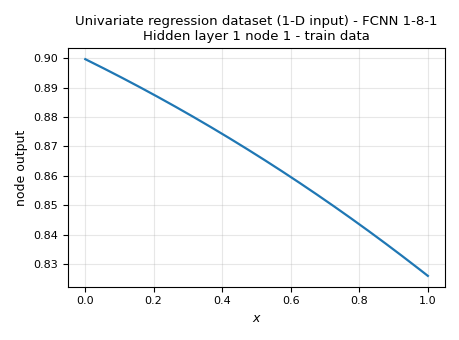
\includegraphics[width=0.323\textwidth]{figures/regression_univariate__best_architecture__node_outputs__hidden_layer1__train__node_001.png}\hfill%
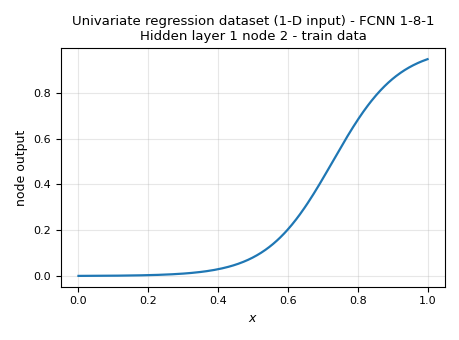
\includegraphics[width=0.323\textwidth]{figures/regression_univariate__best_architecture__node_outputs__hidden_layer1__train__node_002.png}\hfill%
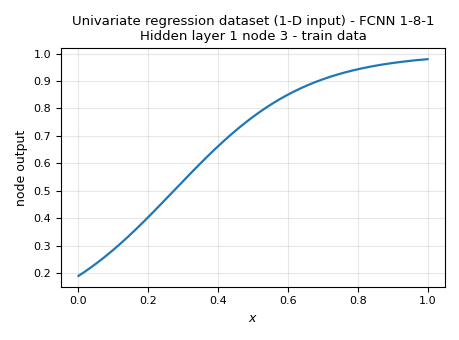
\includegraphics[width=0.323\textwidth]{figures/regression_univariate__best_architecture__node_outputs__hidden_layer1__train__node_003.png}\\[4pt]%
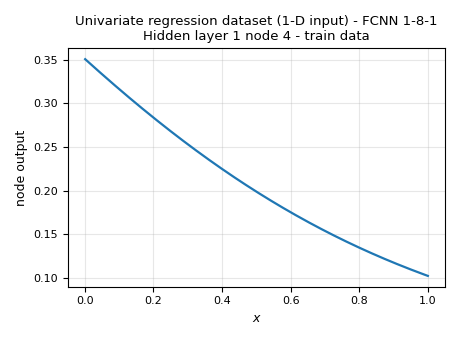
\includegraphics[width=0.323\textwidth]{figures/regression_univariate__best_architecture__node_outputs__hidden_layer1__train__node_004.png}\hfill%
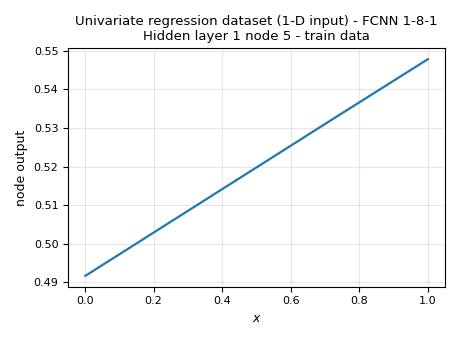
\includegraphics[width=0.323\textwidth]{figures/regression_univariate__best_architecture__node_outputs__hidden_layer1__train__node_005.png}\hfill%
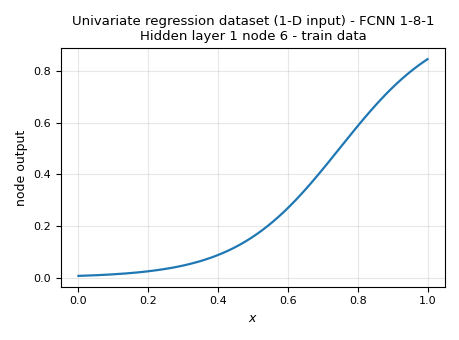
\includegraphics[width=0.323\textwidth]{figures/regression_univariate__best_architecture__node_outputs__hidden_layer1__train__node_006.png}
\caption{Outputs of hidden layer 1 nodes 1--6 of 8 (train data). Each node has its own figure; all 8 are in \texttt{outputs/\allowbreak regression\_\allowbreak univariate/\allowbreak best\_\allowbreak architecture/\allowbreak node\_\allowbreak outputs/\allowbreak hidden\_\allowbreak layer1/\allowbreak train/\allowbreak }.}
\end{figure}

\parahead{Hidden layer 1 --- val data.}
\begin{figure}[H]
\centering
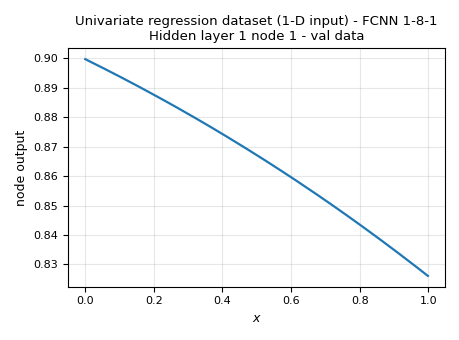
\includegraphics[width=0.323\textwidth]{figures/regression_univariate__best_architecture__node_outputs__hidden_layer1__val__node_001.png}\hfill%
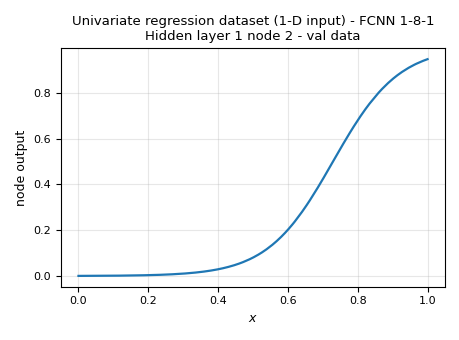
\includegraphics[width=0.323\textwidth]{figures/regression_univariate__best_architecture__node_outputs__hidden_layer1__val__node_002.png}\hfill%
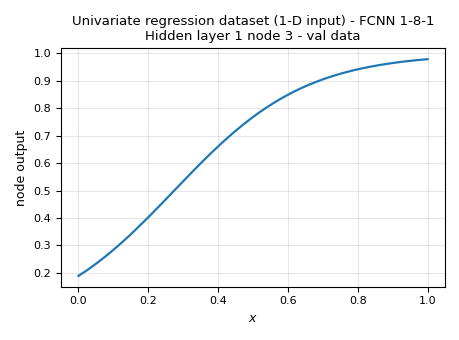
\includegraphics[width=0.323\textwidth]{figures/regression_univariate__best_architecture__node_outputs__hidden_layer1__val__node_003.png}\\[4pt]%
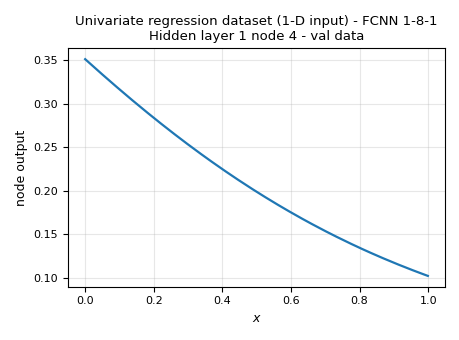
\includegraphics[width=0.323\textwidth]{figures/regression_univariate__best_architecture__node_outputs__hidden_layer1__val__node_004.png}\hfill%
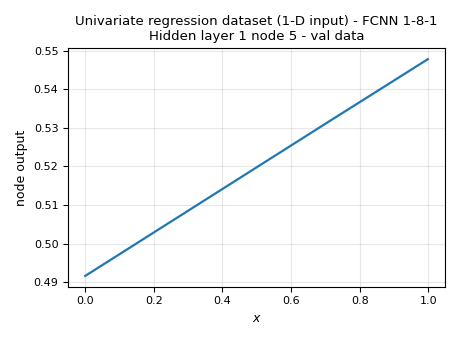
\includegraphics[width=0.323\textwidth]{figures/regression_univariate__best_architecture__node_outputs__hidden_layer1__val__node_005.png}\hfill%
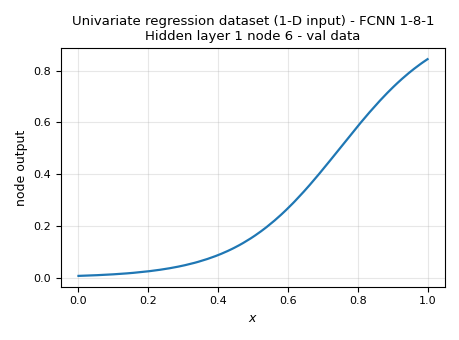
\includegraphics[width=0.323\textwidth]{figures/regression_univariate__best_architecture__node_outputs__hidden_layer1__val__node_006.png}
\caption{Outputs of hidden layer 1 nodes 1--6 of 8 (val data). Each node has its own figure; all 8 are in \texttt{outputs/\allowbreak regression\_\allowbreak univariate/\allowbreak best\_\allowbreak architecture/\allowbreak node\_\allowbreak outputs/\allowbreak hidden\_\allowbreak layer1/\allowbreak val/\allowbreak }.}
\end{figure}

\parahead{Hidden layer 1 --- test data.}
\begin{figure}[H]
\centering
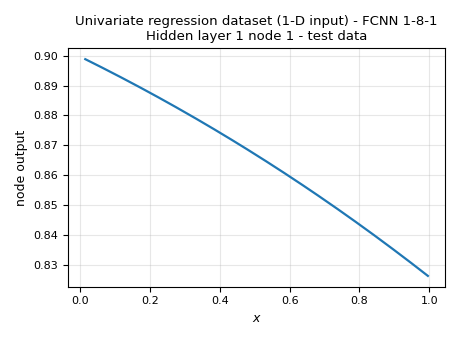
\includegraphics[width=0.323\textwidth]{figures/regression_univariate__best_architecture__node_outputs__hidden_layer1__test__node_001.png}\hfill%
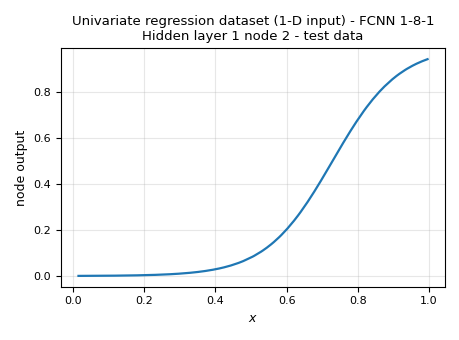
\includegraphics[width=0.323\textwidth]{figures/regression_univariate__best_architecture__node_outputs__hidden_layer1__test__node_002.png}\hfill%
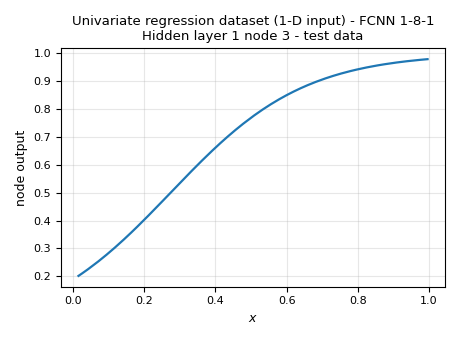
\includegraphics[width=0.323\textwidth]{figures/regression_univariate__best_architecture__node_outputs__hidden_layer1__test__node_003.png}\\[4pt]%
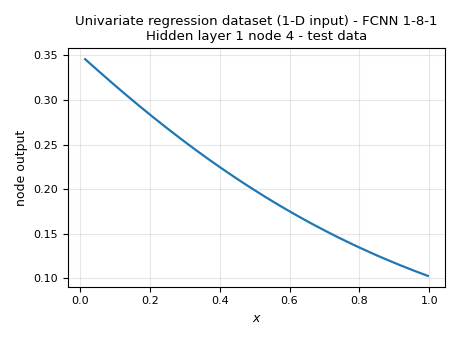
\includegraphics[width=0.323\textwidth]{figures/regression_univariate__best_architecture__node_outputs__hidden_layer1__test__node_004.png}\hfill%
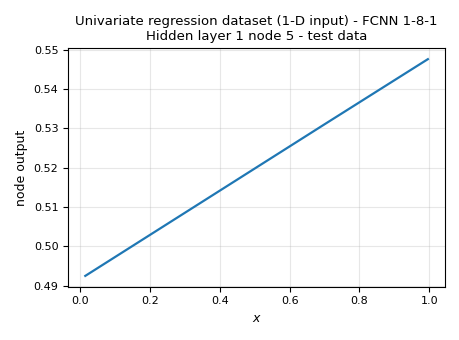
\includegraphics[width=0.323\textwidth]{figures/regression_univariate__best_architecture__node_outputs__hidden_layer1__test__node_005.png}\hfill%
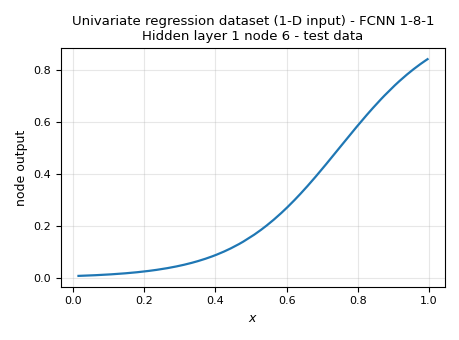
\includegraphics[width=0.323\textwidth]{figures/regression_univariate__best_architecture__node_outputs__hidden_layer1__test__node_006.png}
\caption{Outputs of hidden layer 1 nodes 1--6 of 8 (test data). Each node has its own figure; all 8 are in \texttt{outputs/\allowbreak regression\_\allowbreak univariate/\allowbreak best\_\allowbreak architecture/\allowbreak node\_\allowbreak outputs/\allowbreak hidden\_\allowbreak layer1/\allowbreak test/\allowbreak }.}
\end{figure}

\clearpage

\parahead{Output node --- train data.}
\begin{figure}[H]
\centering
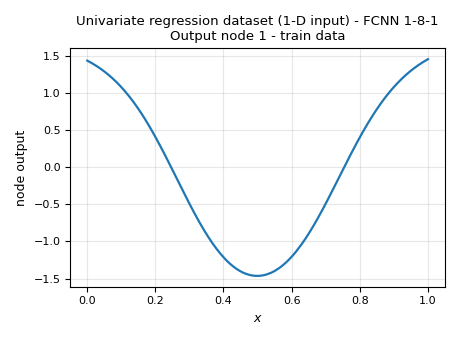
\includegraphics[width=0.323\textwidth]{figures/regression_univariate__best_architecture__node_outputs__output_layer__train__node_001.png}
\caption{Outputs of all 1 output node (train data), one figure per node.}
\end{figure}

\parahead{Output node --- val data.}
\begin{figure}[H]
\centering
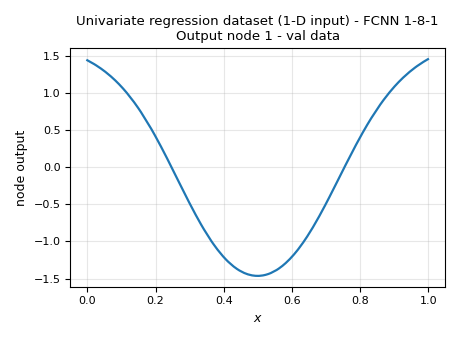
\includegraphics[width=0.323\textwidth]{figures/regression_univariate__best_architecture__node_outputs__output_layer__val__node_001.png}
\caption{Outputs of all 1 output node (val data), one figure per node.}
\end{figure}

\parahead{Output node --- test data.}
\begin{figure}[H]
\centering
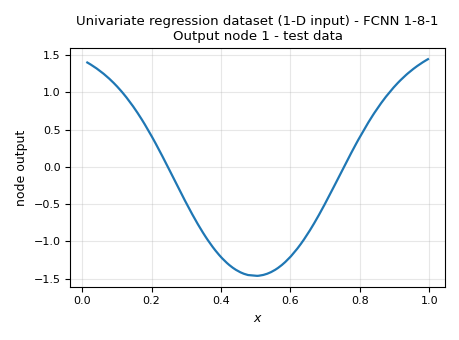
\includegraphics[width=0.323\textwidth]{figures/regression_univariate__best_architecture__node_outputs__output_layer__test__node_001.png}
\caption{Outputs of all 1 output node (test data), one figure per node.}
\end{figure}

\clearpage

\subsection{Comparison with the Single-Neuron Model (Assignment-1)}
The Assignment-1 model --- a single neuron with a linear activation trained by gradient descent --- was retrained on exactly the same split with the same standardisation and scored with the same from-scratch RMSE code.

\begin{table}[H]
\centering
\caption{FCNN against the Assignment-1 single-neuron model.}
\setlength{\tabcolsep}{4pt}
\footnotesize
\resizebox{\textwidth}{!}{%
\begin{tabular}{lrrrrrr}
\toprule
\textbf{Model} & \textbf{RMSE (train)} & \textbf{RMSE (val)} & \textbf{RMSE (test)} & \textbf{\%RMSE (train)} & \textbf{\%RMSE (val)} & \textbf{\%RMSE (test)} \\
\midrule
Single linear neuron & 1.0512 & 1.1349 & 1.0280 & 41.192 & 48.061 & 41.310 \\
\rowcolor{bestrow} \textbf{FCNN 1-8-1 (Assignment-2)} & \textbf{0.0590} & \textbf{0.0625} & \textbf{0.0590} & \textbf{2.314} & \textbf{2.646} & \textbf{2.373} \\
\bottomrule
\end{tabular}
}
\end{table}

\begin{figure}[H]
\centering
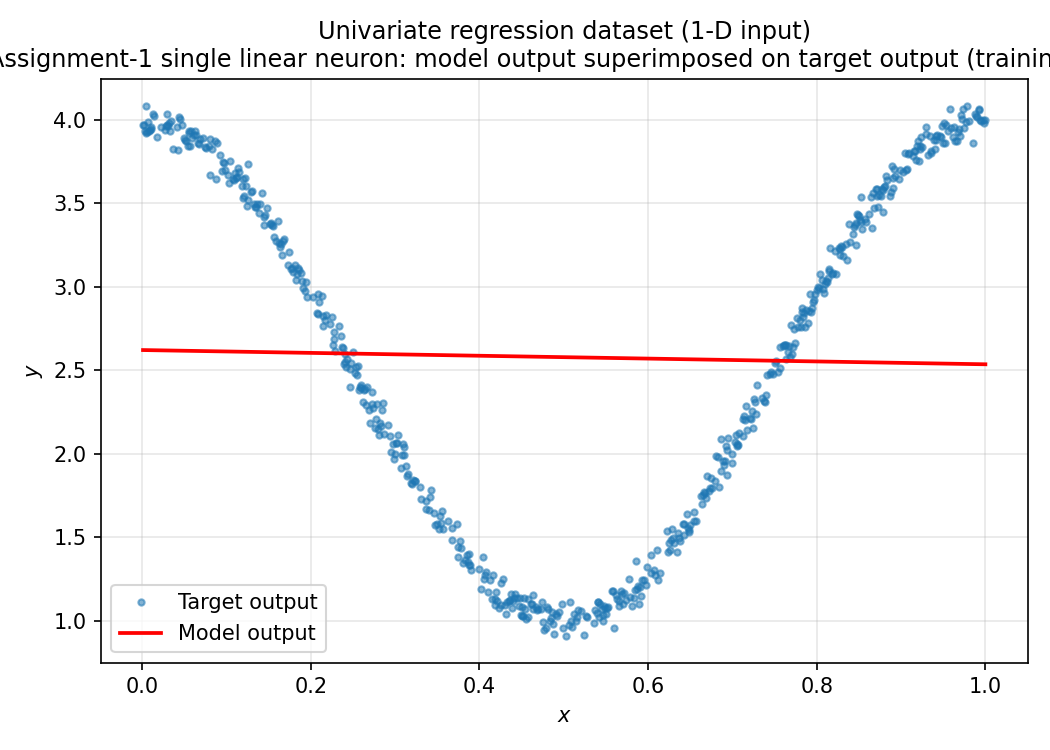
\includegraphics[width=0.8\textwidth,height=9.2cm,keepaspectratio]{figures/regression_univariate__baseline_single_neuron_fit_train.png}
\caption{The Assignment-1 single linear neuron on the same training data.}
\end{figure}

\subsection{Inferences}
\begin{itemize}
  \item The selected architecture is 1-8-1, with a test RMSE of 0.0590 (2.37\% RMSE). Training, validation and test RMSE (0.0590 / 0.0625 / 0.0590) are almost identical, so the selected model generalises and is not overfitted.
  \item The comparison with Assignment-1 is decisive: the single linear neuron reaches a test RMSE of 1.0280 (41.31\%), so the FCNN reduces the test RMSE by 94.3\%. A single linear neuron can only represent a hyperplane, and the target function of this dataset is not linear, so its error is dominated by bias that no amount of further training can remove.
  \item Increasing the number of hidden nodes helps only up to a point. The worst validation RMSE among the architectures tried is 0.0703 (architecture 1-64-1) and the best is 0.0625; beyond the selected size the extra parameters do not lower the validation error, they only make the optimisation slower and noisier. This is the model-complexity trade-off the cross-validation step is meant to expose.
  \item The model-output-vs-target plot shows the network reproducing the curvature of the target function over the whole input range, on training, validation and test data alike; the residual scatter around the curve is the noise in the data, not model error.
  \item The target-vs-model scatter plots lie tightly on the diagonal y = x for all three splits, with no systematic curvature or fan-out, which confirms that the error is unbiased across the output range.
  \item The hidden-node output plots show that each sigmoid hidden node contributes a step / ramp positioned at a different value of x. The linear output node adds these ramps with positive and negative weights, and their sum reproduces the target curve - a direct, visual illustration of why one hidden layer of sigmoid units is a universal approximator.
  \item The average-error curve of the best architecture drops sharply in the first epochs and then decreases very slowly; it ran for 250 epochs. Because the weights are updated after every example, the curve is noticeably noisier than a batch-gradient-descent curve would be, which is the expected signature of SGD.
\end{itemize}

\clearpage

\section{Regression --- Dataset 2 (Bivariate, 2-D Input)}
Model: an FCNN with one and with two hidden layers, logistic hidden nodes and a single linear output node, trained by SGD backpropagation with the squared-error loss and learning rate $\eta = 0.01$. 5 architectures were trained and compared on the validation set.

\subsection{RMSE and \%RMSE for the Different Architectures}
\begin{table}[H]
\centering
\caption{RMSE and \%RMSE on training and validation data for every architecture. The selected architecture is highlighted.}
\setlength{\tabcolsep}{4pt}
\footnotesize
\resizebox{\textwidth}{!}{%
\begin{tabular}{llrrrrrrr}
\toprule
\textbf{Hidden nodes} & \textbf{Architecture} & \textbf{Hidden layers} & \textbf{Params} & \textbf{Epochs} & \textbf{RMSE (train)} & \textbf{\%RMSE (train)} & \textbf{RMSE (val)} & \textbf{\%RMSE (val)} \\
\midrule
16 & 2-16-1 & 1 & 65 & 200 & 0.2292 & 1.121 & 0.1924 & 0.923 \\
32 & 2-32-1 & 1 & 129 & 200 & 0.3452 & 1.688 & 0.3131 & 1.502 \\
64 & 2-64-1 & 1 & 257 & 200 & 0.3765 & 1.841 & 0.3361 & 1.613 \\
32-16 & 2-32-16-1 & 2 & 641 & 200 & 0.1659 & 0.811 & 0.1432 & 0.687 \\
\rowcolor{bestrow} \textbf{64-32} & \textbf{2-64-32-1} & \textbf{2} & \textbf{2305} & \textbf{200} & \textbf{0.1587} & \textbf{0.776} & \textbf{0.1416} & \textbf{0.679} \\
\bottomrule
\end{tabular}
}
\end{table}

\subsection{Best Architecture: 2-64-32-1}
\begin{table}[H]
\centering
\caption{RMSE and \%RMSE of the selected architecture 2-64-32-1 on training, validation and test data.}
\setlength{\tabcolsep}{4pt}
\footnotesize
\begin{tabular}{lrr}
\toprule
\textbf{Data} & \textbf{RMSE} & \textbf{\%RMSE} \\
\midrule
Train & 0.1587 & 0.7760 \\
Val & 0.1416 & 0.6794 \\
Test & 0.1483 & 0.7272 \\
\bottomrule
\end{tabular}
\end{table}

\begin{figure}[H]
\centering
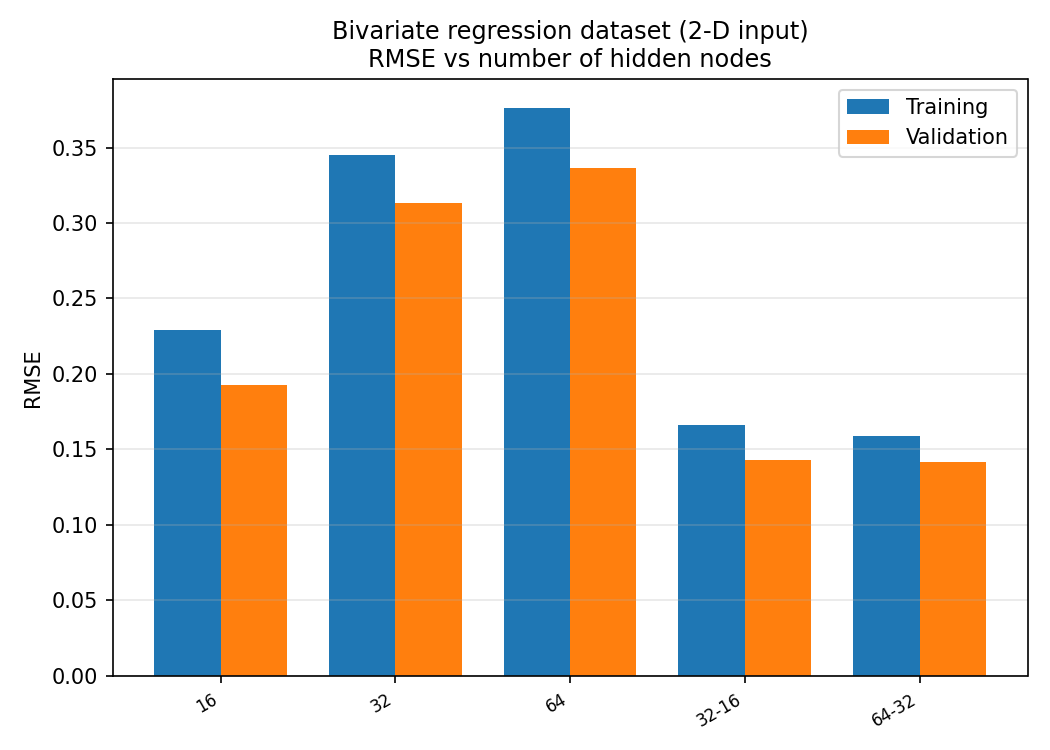
\includegraphics[width=0.78\textwidth,height=7.6cm,keepaspectratio]{figures/regression_bivariate__model_selection_rmse.png}
\caption{RMSE against the number of hidden nodes.}
\end{figure}

Average error against epochs for each architecture that was tried, one graph per architecture. They are deliberately not overlaid on a single axis: with several architectures the curves sit on top of one another and none of them can be read.

\begin{figure}[H]
\centering
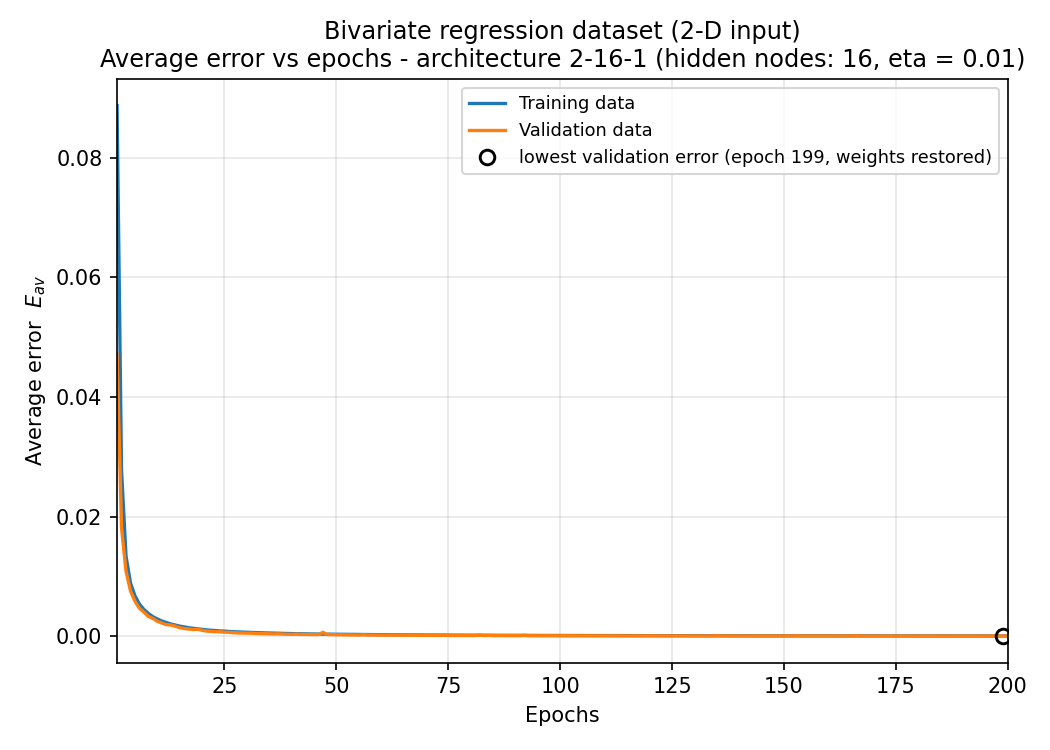
\includegraphics[width=0.78\textwidth,height=7.4cm,keepaspectratio]{figures/regression_bivariate__error_curves__hidden_16.png}
\caption{Average error against epochs, architecture 2-16-1 (hidden nodes: 16).}
\end{figure}

\begin{figure}[H]
\centering
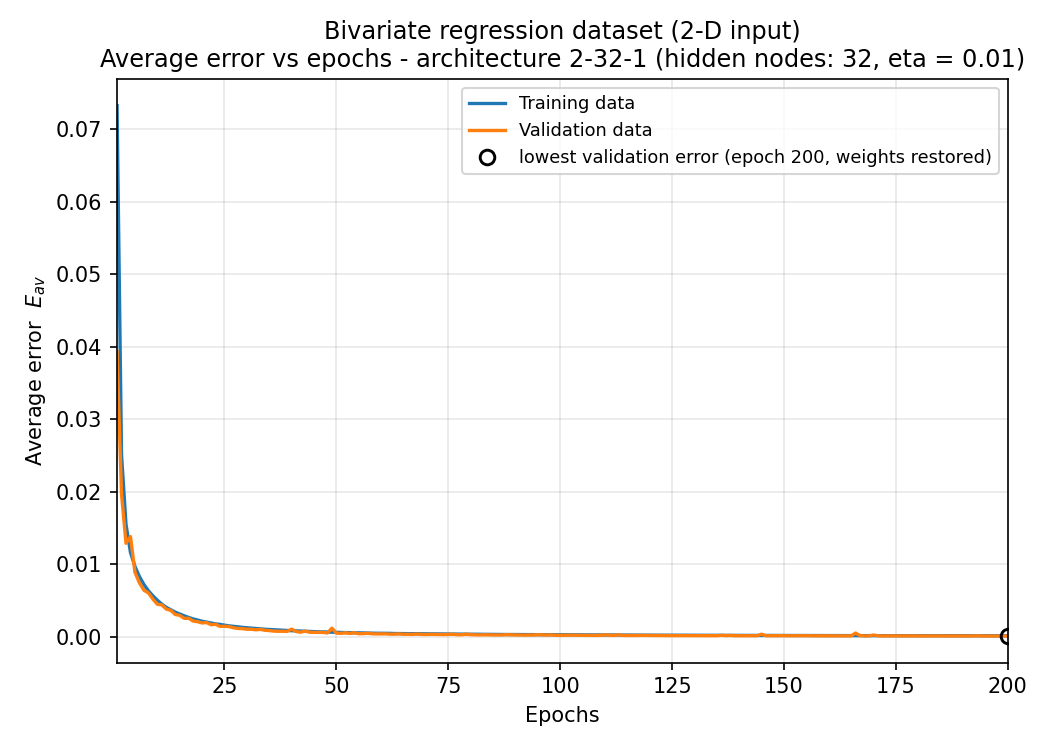
\includegraphics[width=0.78\textwidth,height=7.4cm,keepaspectratio]{figures/regression_bivariate__error_curves__hidden_32.png}
\caption{Average error against epochs, architecture 2-32-1 (hidden nodes: 32).}
\end{figure}

\begin{figure}[H]
\centering
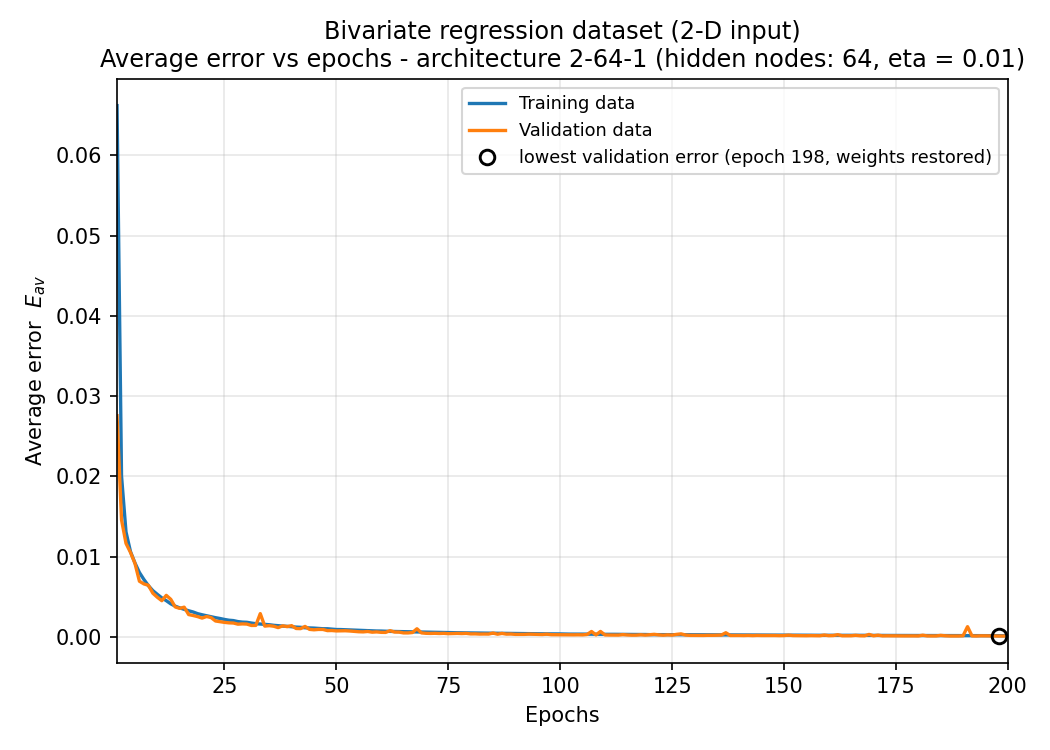
\includegraphics[width=0.78\textwidth,height=7.4cm,keepaspectratio]{figures/regression_bivariate__error_curves__hidden_64.png}
\caption{Average error against epochs, architecture 2-64-1 (hidden nodes: 64).}
\end{figure}

\begin{figure}[H]
\centering
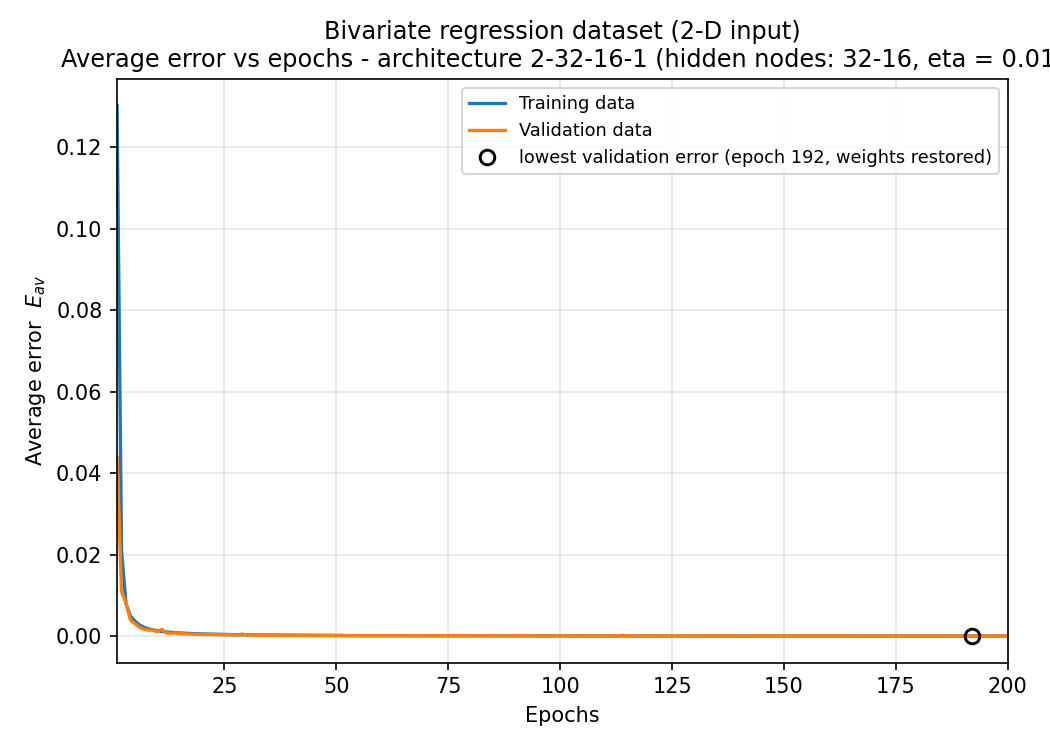
\includegraphics[width=0.78\textwidth,height=7.4cm,keepaspectratio]{figures/regression_bivariate__error_curves__hidden_32-16.png}
\caption{Average error against epochs, architecture 2-32-16-1 (hidden nodes: 32-16).}
\end{figure}

\begin{figure}[H]
\centering
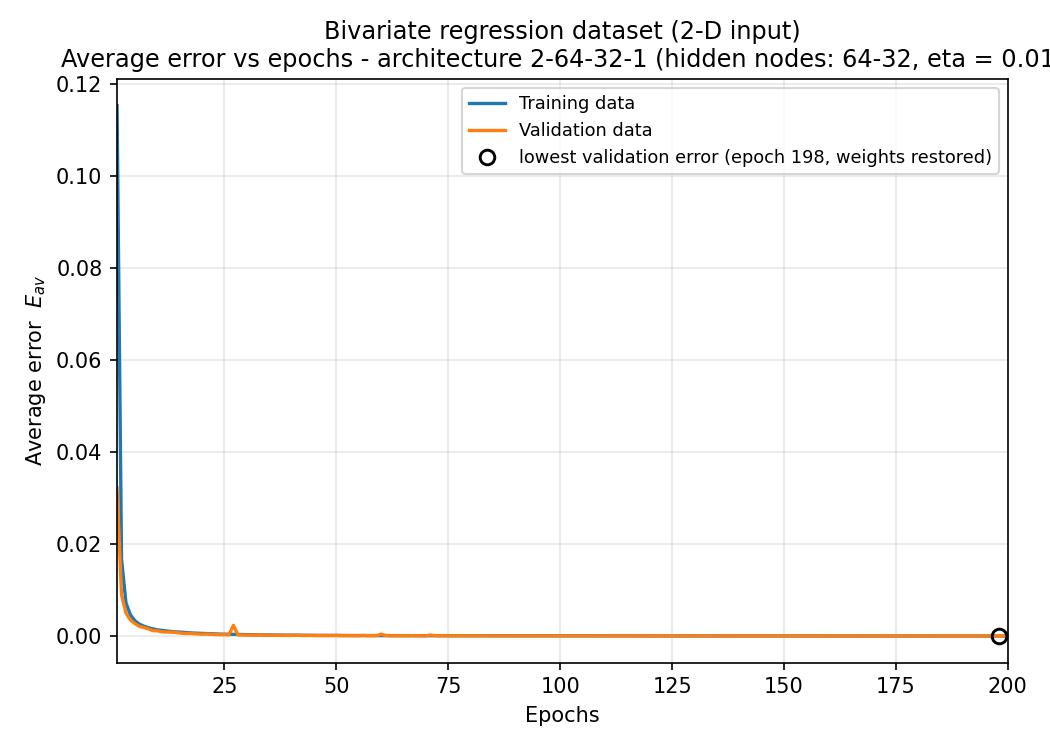
\includegraphics[width=0.78\textwidth,height=7.4cm,keepaspectratio]{figures/regression_bivariate__error_curves__hidden_64-32.png}
\caption{Average error against epochs, architecture 2-64-32-1 (hidden nodes: 64-32).}
\end{figure}

\clearpage

\parahead{Average error against epochs (best architecture).}
\begin{figure}[H]
\centering
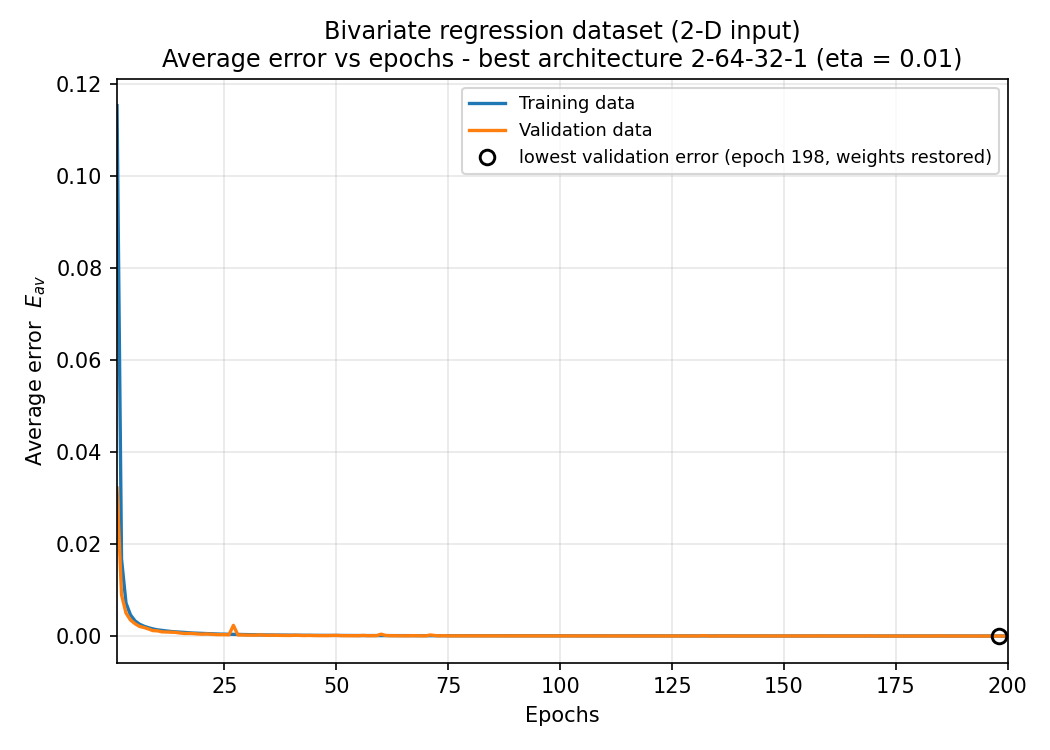
\includegraphics[width=0.8\textwidth,height=8.4cm,keepaspectratio]{figures/regression_bivariate__best_architecture__error_vs_epochs.png}
\caption{Average error $E_{\mathrm{av}}$ against epochs for the best architecture.}
\end{figure}

\subsection{Model Output Superimposed on the Target Output}
In the plots below the two base axes are $x_{1}$ and $x_{2}$ and the vertical axis is the target / model output.

\begin{figure}[H]
\centering
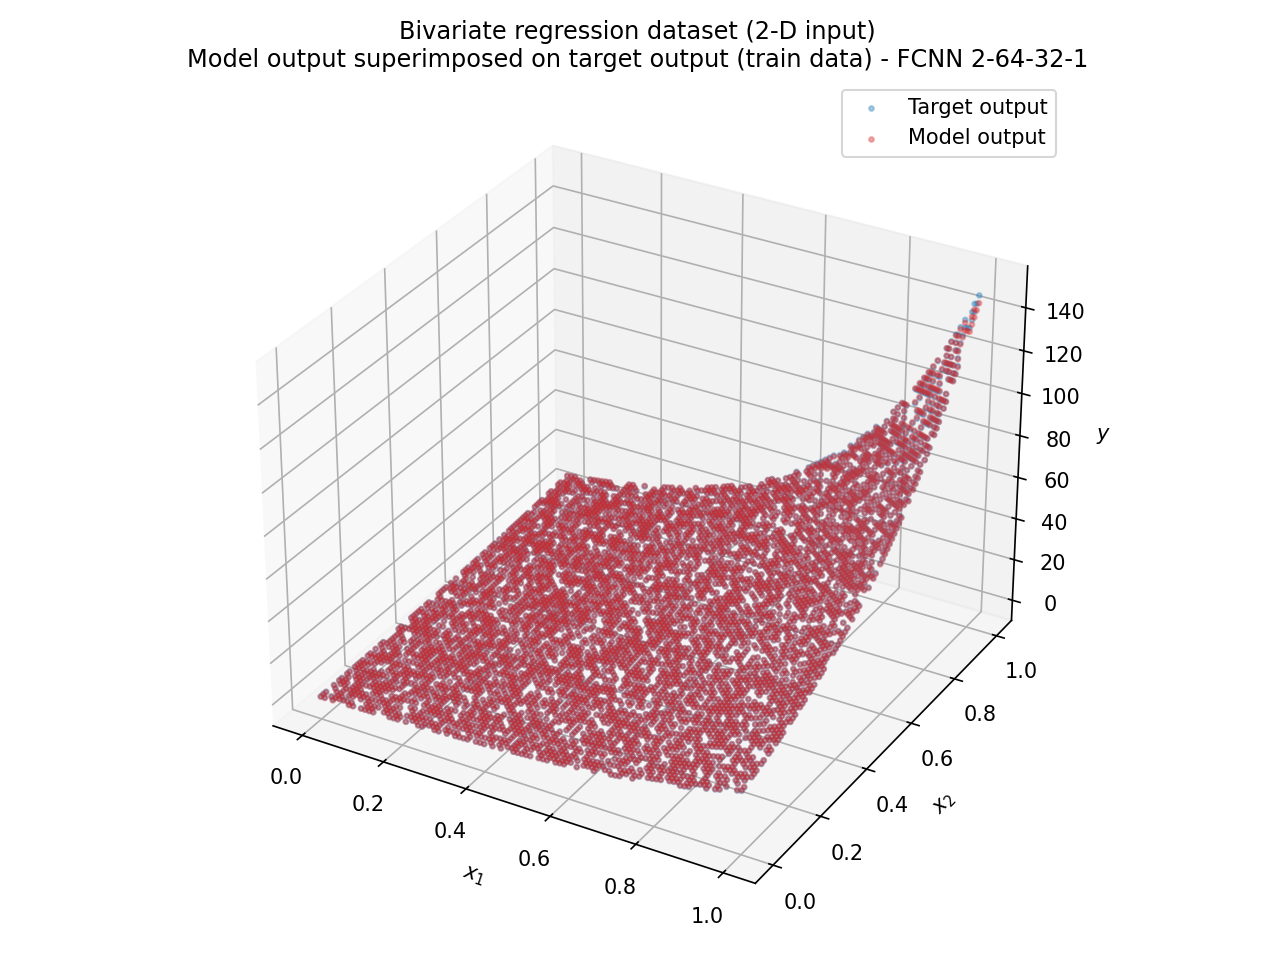
\includegraphics[width=0.8\textwidth,height=9.2cm,keepaspectratio]{figures/regression_bivariate__best_architecture__model_vs_target_train.png}
\caption{Model output superimposed on the target output (train data).}
\end{figure}

\begin{figure}[H]
\centering
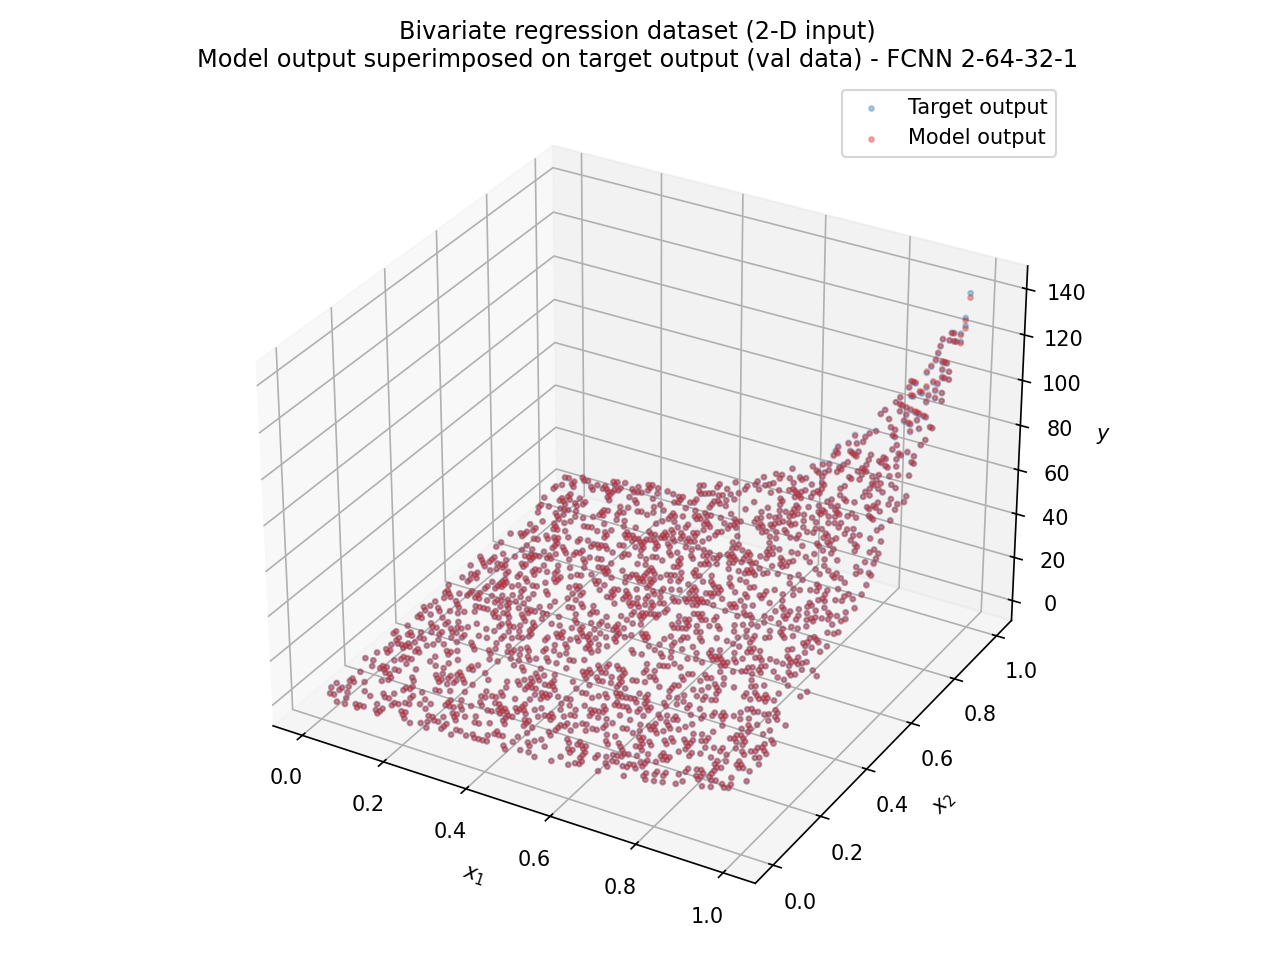
\includegraphics[width=0.8\textwidth,height=9.2cm,keepaspectratio]{figures/regression_bivariate__best_architecture__model_vs_target_val.png}
\caption{Model output superimposed on the target output (val data).}
\end{figure}

\begin{figure}[H]
\centering
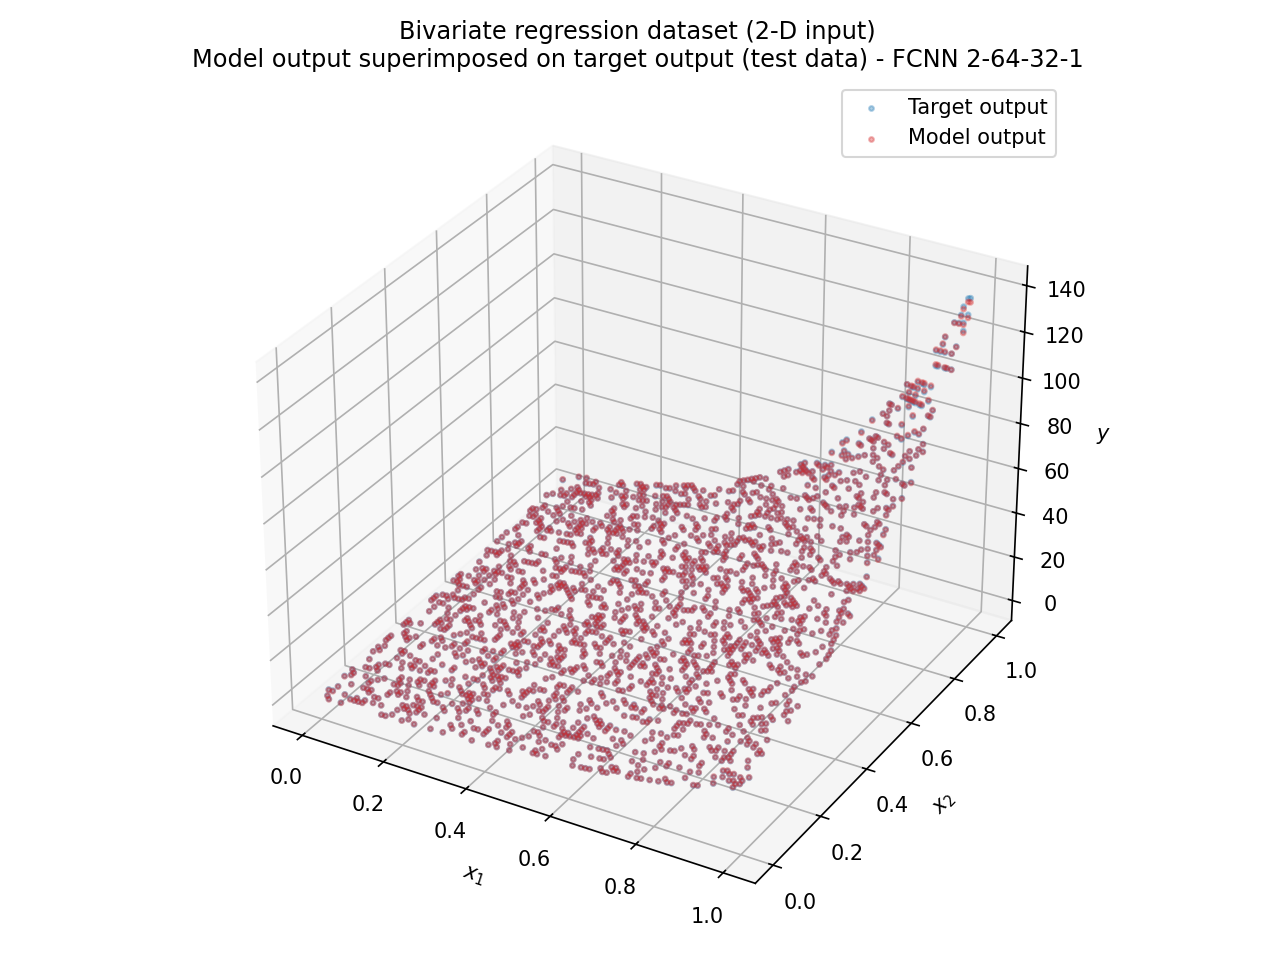
\includegraphics[width=0.8\textwidth,height=9.2cm,keepaspectratio]{figures/regression_bivariate__best_architecture__model_vs_target_test.png}
\caption{Model output superimposed on the target output (test data).}
\end{figure}

\clearpage

\subsection{Scatter Plot of Target Output against Model Output}
\begin{figure}[H]
\centering
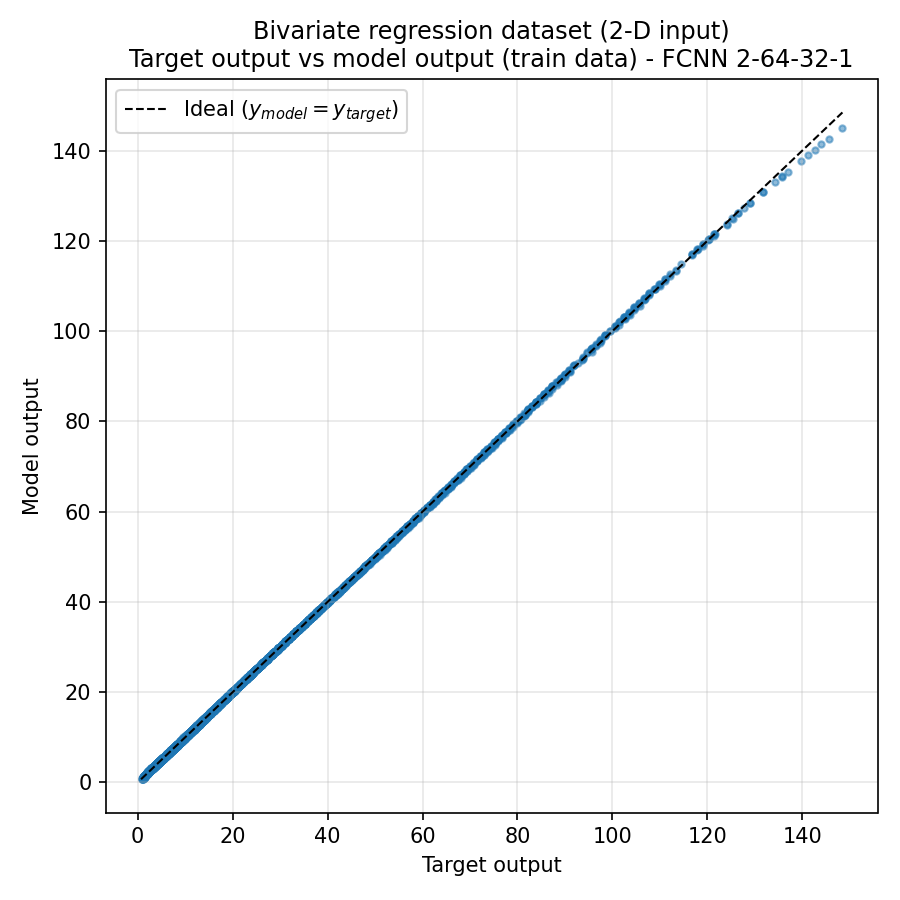
\includegraphics[width=0.66\textwidth,height=8.0cm,keepaspectratio]{figures/regression_bivariate__best_architecture__scatter_target_vs_model_train.png}
\caption{Target output (horizontal axis) against model output (vertical axis), train data.}
\end{figure}

\begin{figure}[H]
\centering
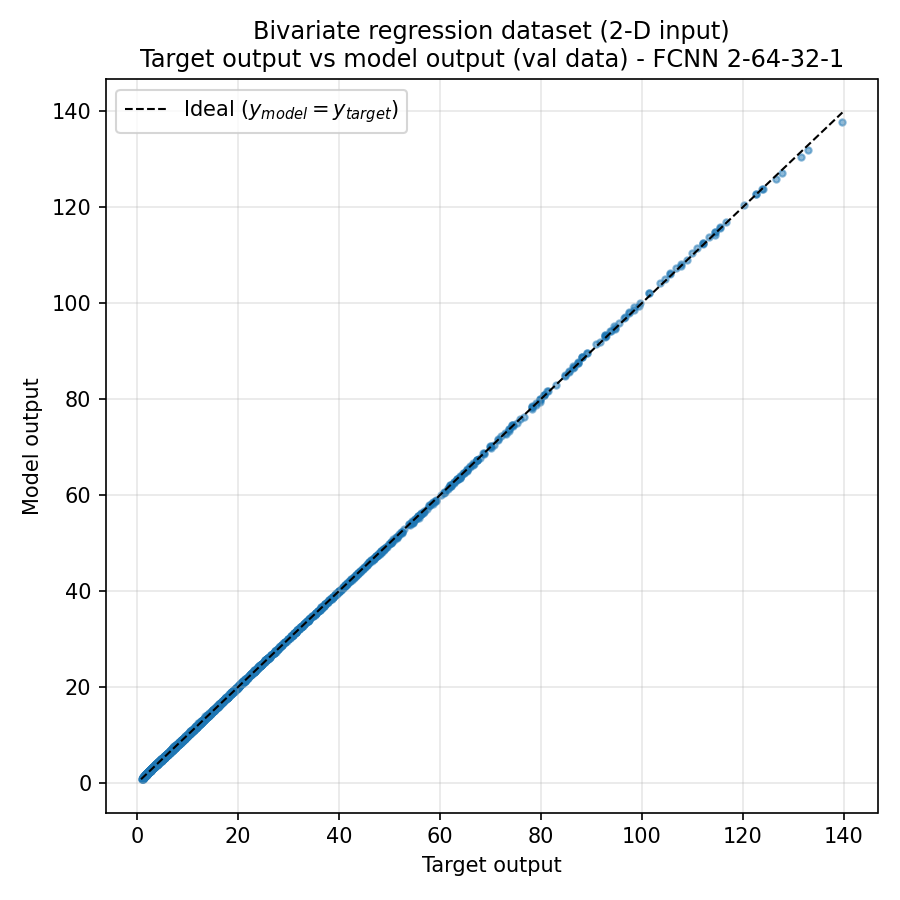
\includegraphics[width=0.66\textwidth,height=8.0cm,keepaspectratio]{figures/regression_bivariate__best_architecture__scatter_target_vs_model_val.png}
\caption{Target output (horizontal axis) against model output (vertical axis), val data.}
\end{figure}

\begin{figure}[H]
\centering
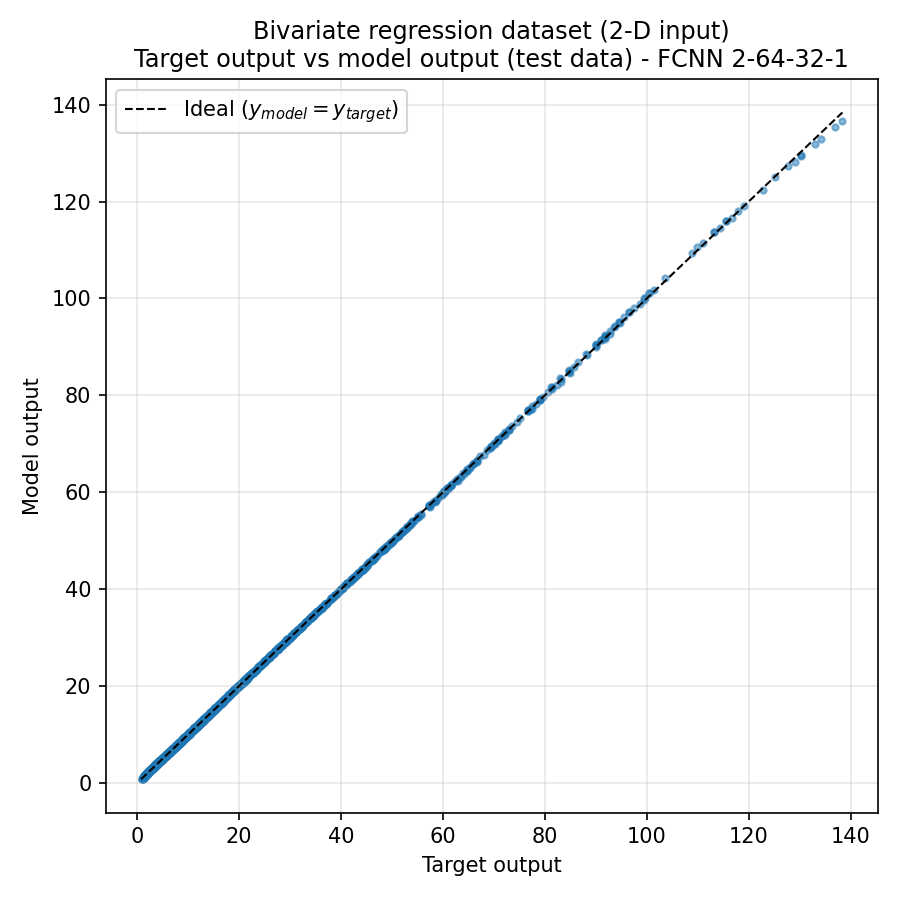
\includegraphics[width=0.66\textwidth,height=8.0cm,keepaspectratio]{figures/regression_bivariate__best_architecture__scatter_target_vs_model_test.png}
\caption{Target output (horizontal axis) against model output (vertical axis), test data.}
\end{figure}

\clearpage

\subsection{Outputs of the Hidden Nodes and Output Node}
Every hidden node and the output node is plotted in its own figure: the vertical axis is the output of that node and the remaining axes are the input variables of each example. The selected network has 97 nodes in total, so the complete set is 291 figures (one per node per split); they are all written to \texttt{outputs/\allowbreak regression\_\allowbreak bivariate/\allowbreak best\_\allowbreak architecture/\allowbreak node\_\allowbreak outputs/\allowbreak }. The first 6 nodes of each layer are reproduced below for each split.

\parahead{Hidden layer 1 --- train data.}
\begin{figure}[H]
\centering
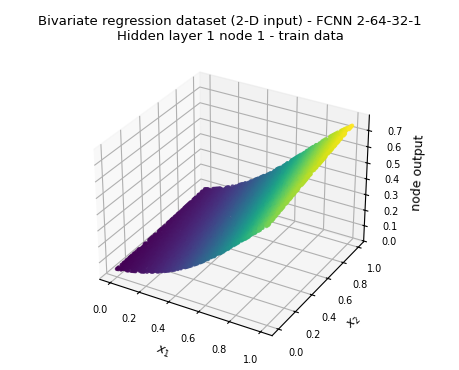
\includegraphics[width=0.323\textwidth]{figures/regression_bivariate__best_architecture__node_outputs__hidden_layer1__train__node_001.png}\hfill%
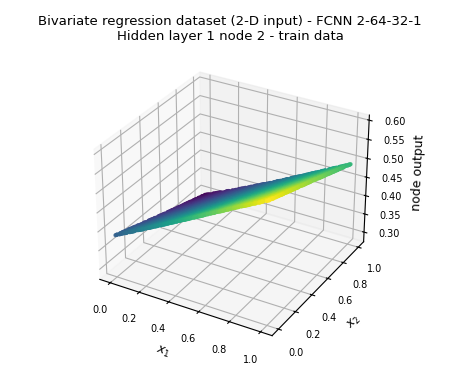
\includegraphics[width=0.323\textwidth]{figures/regression_bivariate__best_architecture__node_outputs__hidden_layer1__train__node_002.png}\hfill%
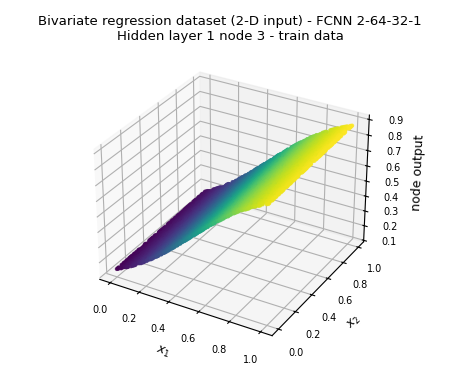
\includegraphics[width=0.323\textwidth]{figures/regression_bivariate__best_architecture__node_outputs__hidden_layer1__train__node_003.png}\\[4pt]%
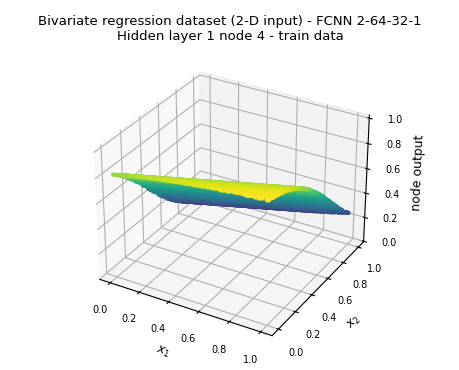
\includegraphics[width=0.323\textwidth]{figures/regression_bivariate__best_architecture__node_outputs__hidden_layer1__train__node_004.png}\hfill%
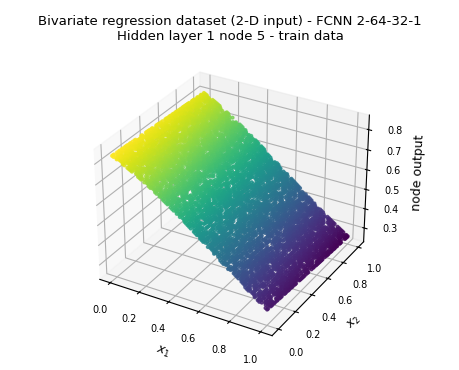
\includegraphics[width=0.323\textwidth]{figures/regression_bivariate__best_architecture__node_outputs__hidden_layer1__train__node_005.png}\hfill%
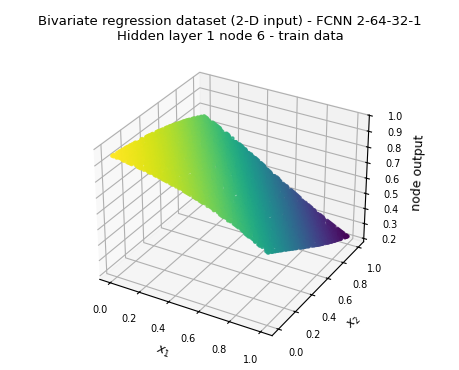
\includegraphics[width=0.323\textwidth]{figures/regression_bivariate__best_architecture__node_outputs__hidden_layer1__train__node_006.png}
\caption{Outputs of hidden layer 1 nodes 1--6 of 64 (train data). Each node has its own figure; all 64 are in \texttt{outputs/\allowbreak regression\_\allowbreak bivariate/\allowbreak best\_\allowbreak architecture/\allowbreak node\_\allowbreak outputs/\allowbreak hidden\_\allowbreak layer1/\allowbreak train/\allowbreak }.}
\end{figure}

\parahead{Hidden layer 1 --- val data.}
\begin{figure}[H]
\centering
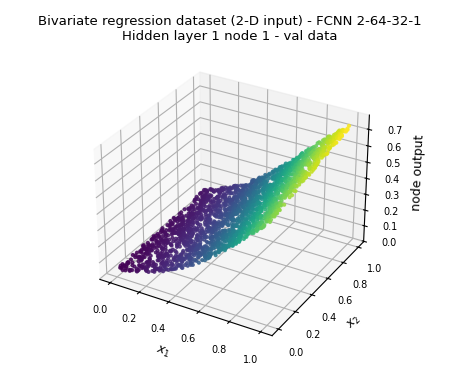
\includegraphics[width=0.323\textwidth]{figures/regression_bivariate__best_architecture__node_outputs__hidden_layer1__val__node_001.png}\hfill%
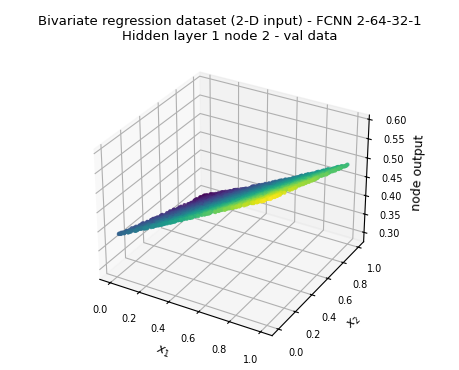
\includegraphics[width=0.323\textwidth]{figures/regression_bivariate__best_architecture__node_outputs__hidden_layer1__val__node_002.png}\hfill%
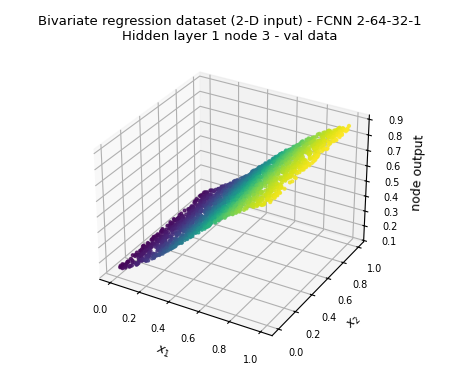
\includegraphics[width=0.323\textwidth]{figures/regression_bivariate__best_architecture__node_outputs__hidden_layer1__val__node_003.png}\\[4pt]%
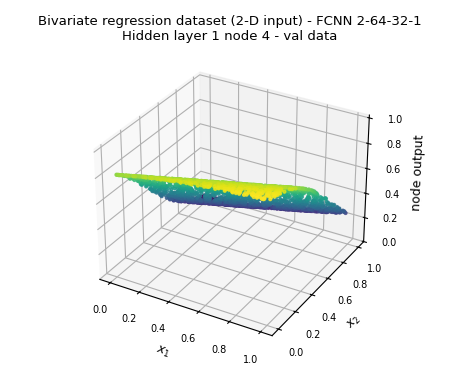
\includegraphics[width=0.323\textwidth]{figures/regression_bivariate__best_architecture__node_outputs__hidden_layer1__val__node_004.png}\hfill%
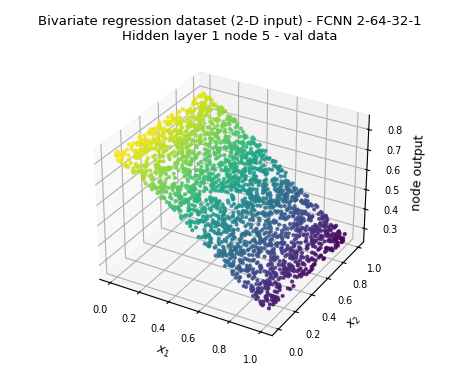
\includegraphics[width=0.323\textwidth]{figures/regression_bivariate__best_architecture__node_outputs__hidden_layer1__val__node_005.png}\hfill%
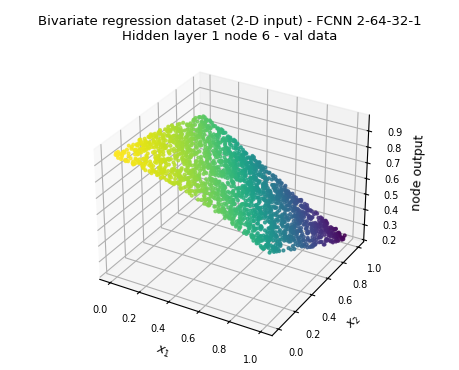
\includegraphics[width=0.323\textwidth]{figures/regression_bivariate__best_architecture__node_outputs__hidden_layer1__val__node_006.png}
\caption{Outputs of hidden layer 1 nodes 1--6 of 64 (val data). Each node has its own figure; all 64 are in \texttt{outputs/\allowbreak regression\_\allowbreak bivariate/\allowbreak best\_\allowbreak architecture/\allowbreak node\_\allowbreak outputs/\allowbreak hidden\_\allowbreak layer1/\allowbreak val/\allowbreak }.}
\end{figure}

\parahead{Hidden layer 1 --- test data.}
\begin{figure}[H]
\centering
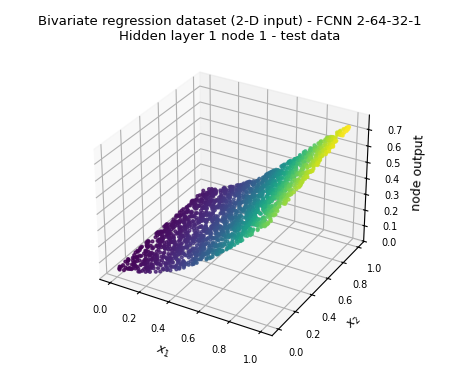
\includegraphics[width=0.323\textwidth]{figures/regression_bivariate__best_architecture__node_outputs__hidden_layer1__test__node_001.png}\hfill%
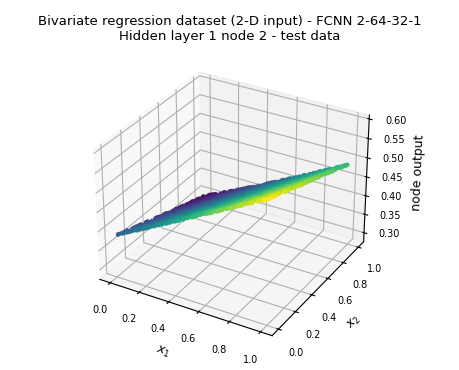
\includegraphics[width=0.323\textwidth]{figures/regression_bivariate__best_architecture__node_outputs__hidden_layer1__test__node_002.png}\hfill%
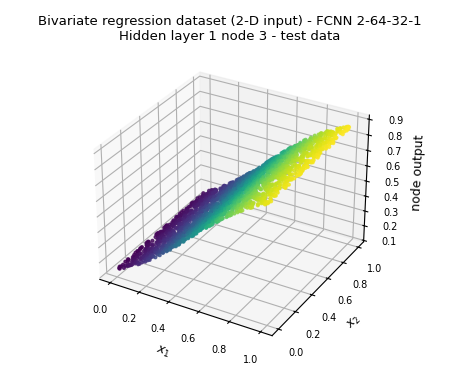
\includegraphics[width=0.323\textwidth]{figures/regression_bivariate__best_architecture__node_outputs__hidden_layer1__test__node_003.png}\\[4pt]%
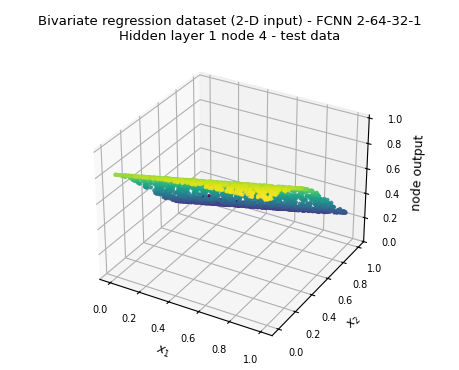
\includegraphics[width=0.323\textwidth]{figures/regression_bivariate__best_architecture__node_outputs__hidden_layer1__test__node_004.png}\hfill%
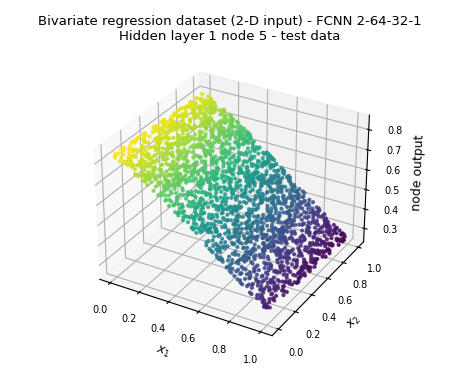
\includegraphics[width=0.323\textwidth]{figures/regression_bivariate__best_architecture__node_outputs__hidden_layer1__test__node_005.png}\hfill%
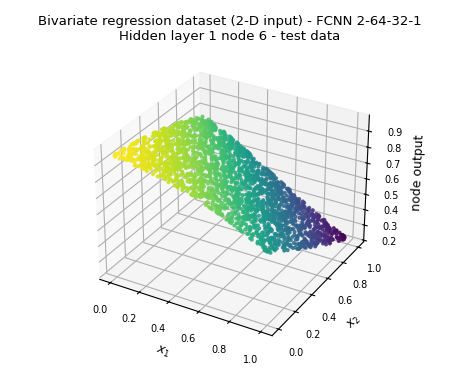
\includegraphics[width=0.323\textwidth]{figures/regression_bivariate__best_architecture__node_outputs__hidden_layer1__test__node_006.png}
\caption{Outputs of hidden layer 1 nodes 1--6 of 64 (test data). Each node has its own figure; all 64 are in \texttt{outputs/\allowbreak regression\_\allowbreak bivariate/\allowbreak best\_\allowbreak architecture/\allowbreak node\_\allowbreak outputs/\allowbreak hidden\_\allowbreak layer1/\allowbreak test/\allowbreak }.}
\end{figure}

\clearpage

\parahead{Hidden layer 2 --- train data.}
\begin{figure}[H]
\centering
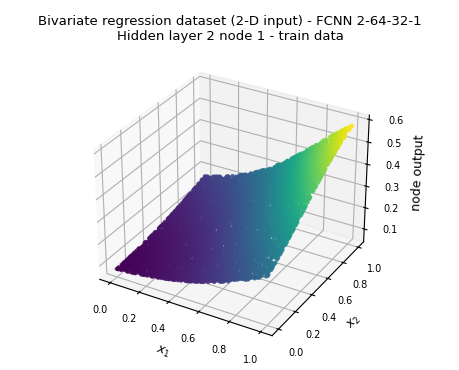
\includegraphics[width=0.323\textwidth]{figures/regression_bivariate__best_architecture__node_outputs__hidden_layer2__train__node_001.png}\hfill%
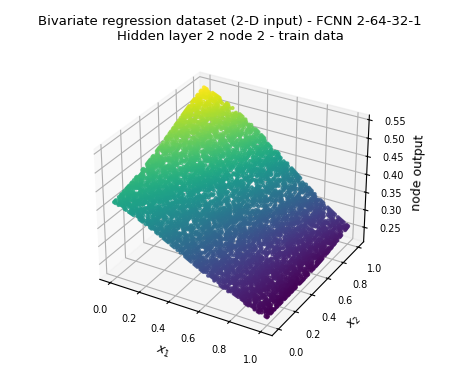
\includegraphics[width=0.323\textwidth]{figures/regression_bivariate__best_architecture__node_outputs__hidden_layer2__train__node_002.png}\hfill%
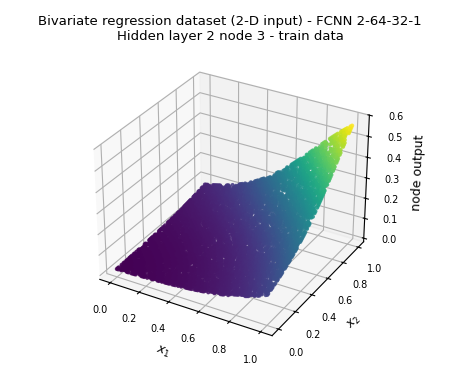
\includegraphics[width=0.323\textwidth]{figures/regression_bivariate__best_architecture__node_outputs__hidden_layer2__train__node_003.png}\\[4pt]%
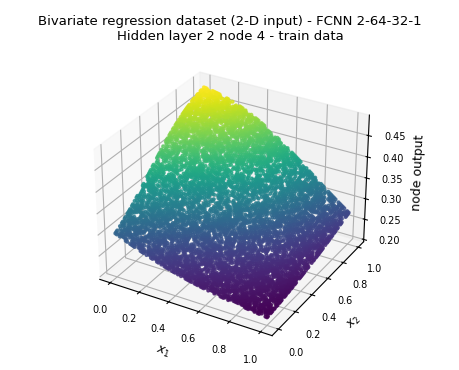
\includegraphics[width=0.323\textwidth]{figures/regression_bivariate__best_architecture__node_outputs__hidden_layer2__train__node_004.png}\hfill%
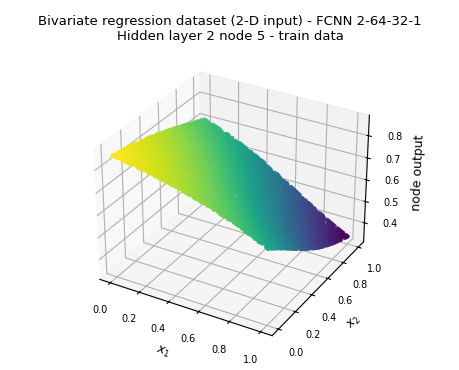
\includegraphics[width=0.323\textwidth]{figures/regression_bivariate__best_architecture__node_outputs__hidden_layer2__train__node_005.png}\hfill%
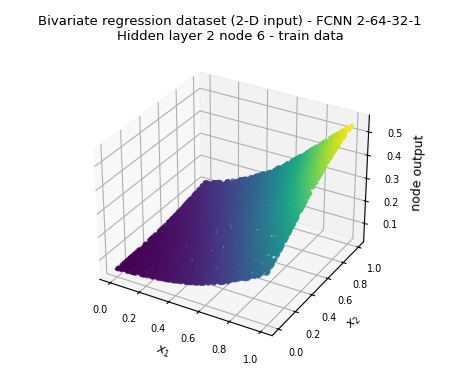
\includegraphics[width=0.323\textwidth]{figures/regression_bivariate__best_architecture__node_outputs__hidden_layer2__train__node_006.png}
\caption{Outputs of hidden layer 2 nodes 1--6 of 32 (train data). Each node has its own figure; all 32 are in \texttt{outputs/\allowbreak regression\_\allowbreak bivariate/\allowbreak best\_\allowbreak architecture/\allowbreak node\_\allowbreak outputs/\allowbreak hidden\_\allowbreak layer2/\allowbreak train/\allowbreak }.}
\end{figure}

\parahead{Hidden layer 2 --- val data.}
\begin{figure}[H]
\centering
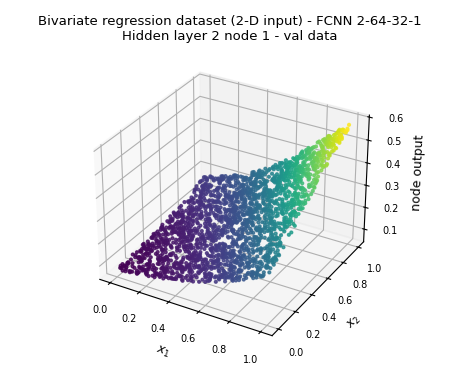
\includegraphics[width=0.323\textwidth]{figures/regression_bivariate__best_architecture__node_outputs__hidden_layer2__val__node_001.png}\hfill%
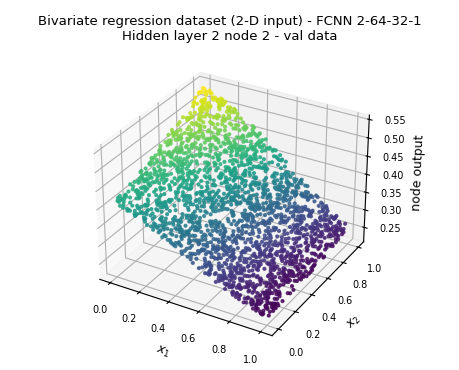
\includegraphics[width=0.323\textwidth]{figures/regression_bivariate__best_architecture__node_outputs__hidden_layer2__val__node_002.png}\hfill%
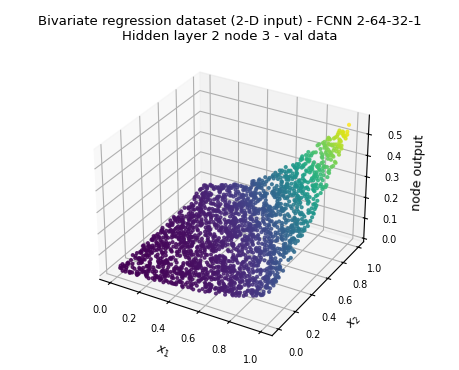
\includegraphics[width=0.323\textwidth]{figures/regression_bivariate__best_architecture__node_outputs__hidden_layer2__val__node_003.png}\\[4pt]%
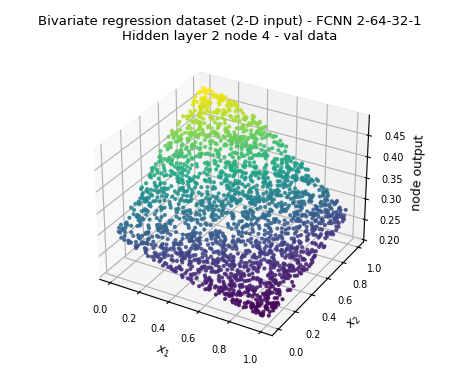
\includegraphics[width=0.323\textwidth]{figures/regression_bivariate__best_architecture__node_outputs__hidden_layer2__val__node_004.png}\hfill%
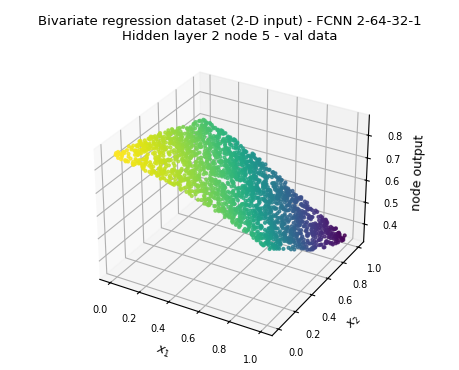
\includegraphics[width=0.323\textwidth]{figures/regression_bivariate__best_architecture__node_outputs__hidden_layer2__val__node_005.png}\hfill%
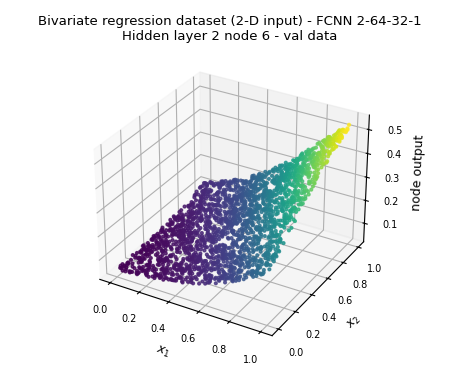
\includegraphics[width=0.323\textwidth]{figures/regression_bivariate__best_architecture__node_outputs__hidden_layer2__val__node_006.png}
\caption{Outputs of hidden layer 2 nodes 1--6 of 32 (val data). Each node has its own figure; all 32 are in \texttt{outputs/\allowbreak regression\_\allowbreak bivariate/\allowbreak best\_\allowbreak architecture/\allowbreak node\_\allowbreak outputs/\allowbreak hidden\_\allowbreak layer2/\allowbreak val/\allowbreak }.}
\end{figure}

\parahead{Hidden layer 2 --- test data.}
\begin{figure}[H]
\centering
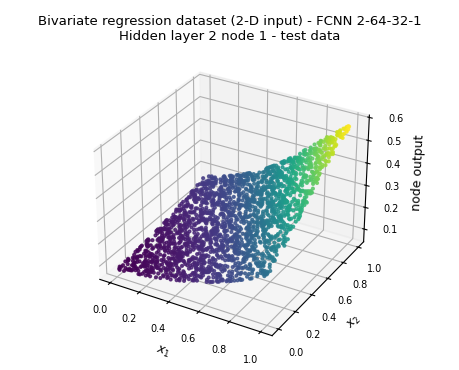
\includegraphics[width=0.323\textwidth]{figures/regression_bivariate__best_architecture__node_outputs__hidden_layer2__test__node_001.png}\hfill%
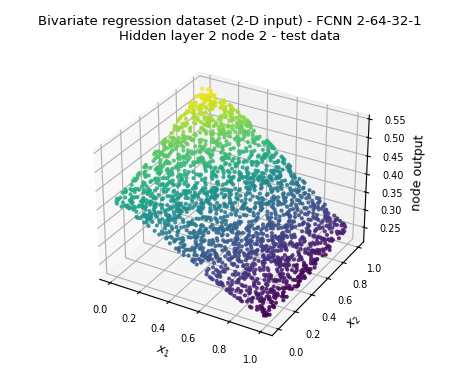
\includegraphics[width=0.323\textwidth]{figures/regression_bivariate__best_architecture__node_outputs__hidden_layer2__test__node_002.png}\hfill%
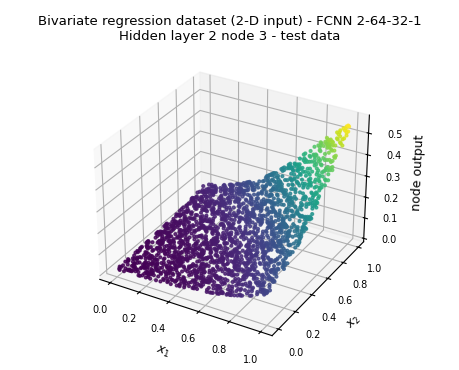
\includegraphics[width=0.323\textwidth]{figures/regression_bivariate__best_architecture__node_outputs__hidden_layer2__test__node_003.png}\\[4pt]%
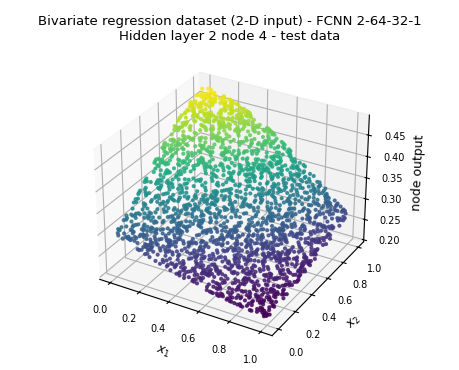
\includegraphics[width=0.323\textwidth]{figures/regression_bivariate__best_architecture__node_outputs__hidden_layer2__test__node_004.png}\hfill%
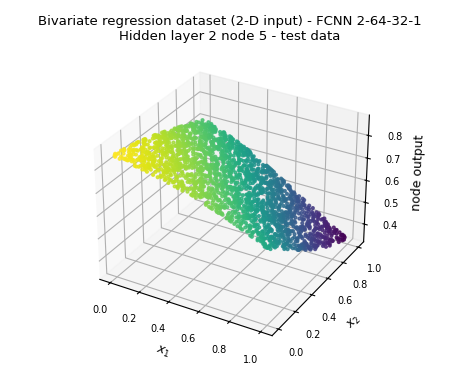
\includegraphics[width=0.323\textwidth]{figures/regression_bivariate__best_architecture__node_outputs__hidden_layer2__test__node_005.png}\hfill%
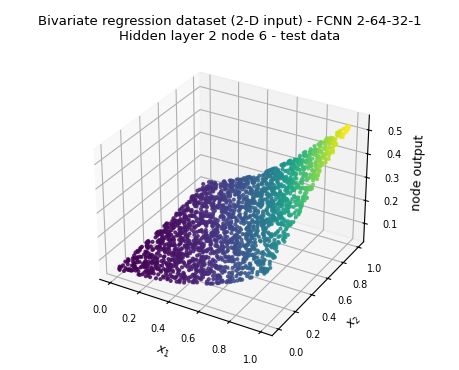
\includegraphics[width=0.323\textwidth]{figures/regression_bivariate__best_architecture__node_outputs__hidden_layer2__test__node_006.png}
\caption{Outputs of hidden layer 2 nodes 1--6 of 32 (test data). Each node has its own figure; all 32 are in \texttt{outputs/\allowbreak regression\_\allowbreak bivariate/\allowbreak best\_\allowbreak architecture/\allowbreak node\_\allowbreak outputs/\allowbreak hidden\_\allowbreak layer2/\allowbreak test/\allowbreak }.}
\end{figure}

\clearpage

\parahead{Output node --- train data.}
\begin{figure}[H]
\centering
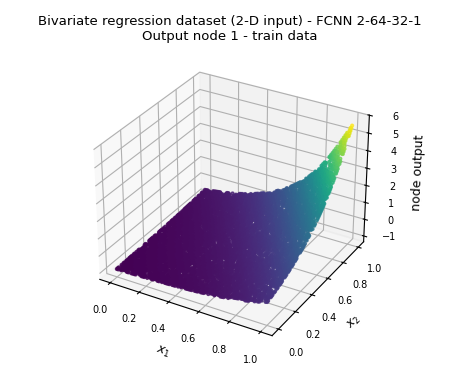
\includegraphics[width=0.323\textwidth]{figures/regression_bivariate__best_architecture__node_outputs__output_layer__train__node_001.png}
\caption{Outputs of all 1 output node (train data), one figure per node.}
\end{figure}

\parahead{Output node --- val data.}
\begin{figure}[H]
\centering
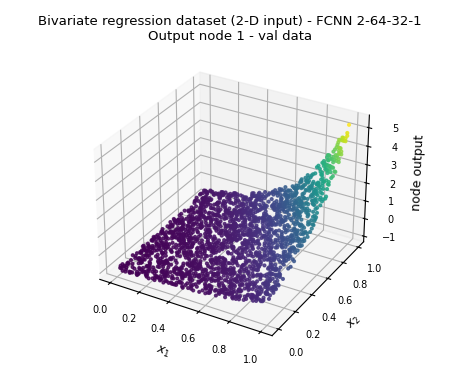
\includegraphics[width=0.323\textwidth]{figures/regression_bivariate__best_architecture__node_outputs__output_layer__val__node_001.png}
\caption{Outputs of all 1 output node (val data), one figure per node.}
\end{figure}

\parahead{Output node --- test data.}
\begin{figure}[H]
\centering
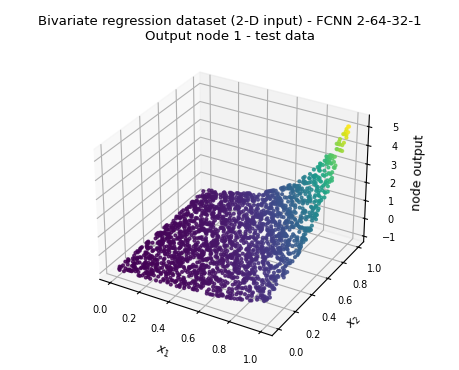
\includegraphics[width=0.323\textwidth]{figures/regression_bivariate__best_architecture__node_outputs__output_layer__test__node_001.png}
\caption{Outputs of all 1 output node (test data), one figure per node.}
\end{figure}

\clearpage

\subsection{Comparison with the Single-Neuron Model (Assignment-1)}
The Assignment-1 model --- a single neuron with a linear activation trained by gradient descent --- was retrained on exactly the same split with the same standardisation and scored with the same from-scratch RMSE code.

\begin{table}[H]
\centering
\caption{FCNN against the Assignment-1 single-neuron model.}
\setlength{\tabcolsep}{4pt}
\footnotesize
\resizebox{\textwidth}{!}{%
\begin{tabular}{lrrrrrr}
\toprule
\textbf{Model} & \textbf{RMSE (train)} & \textbf{RMSE (val)} & \textbf{RMSE (test)} & \textbf{\%RMSE (train)} & \textbf{\%RMSE (val)} & \textbf{\%RMSE (test)} \\
\midrule
Single linear neuron & 11.5134 & 11.7742 & 11.5259 & 56.297 & 56.481 & 56.508 \\
\rowcolor{bestrow} \textbf{FCNN 2-64-32-1 (Assignment-2)} & \textbf{0.1587} & \textbf{0.1416} & \textbf{0.1483} & \textbf{0.776} & \textbf{0.679} & \textbf{0.727} \\
\bottomrule
\end{tabular}
}
\end{table}

\begin{figure}[H]
\centering
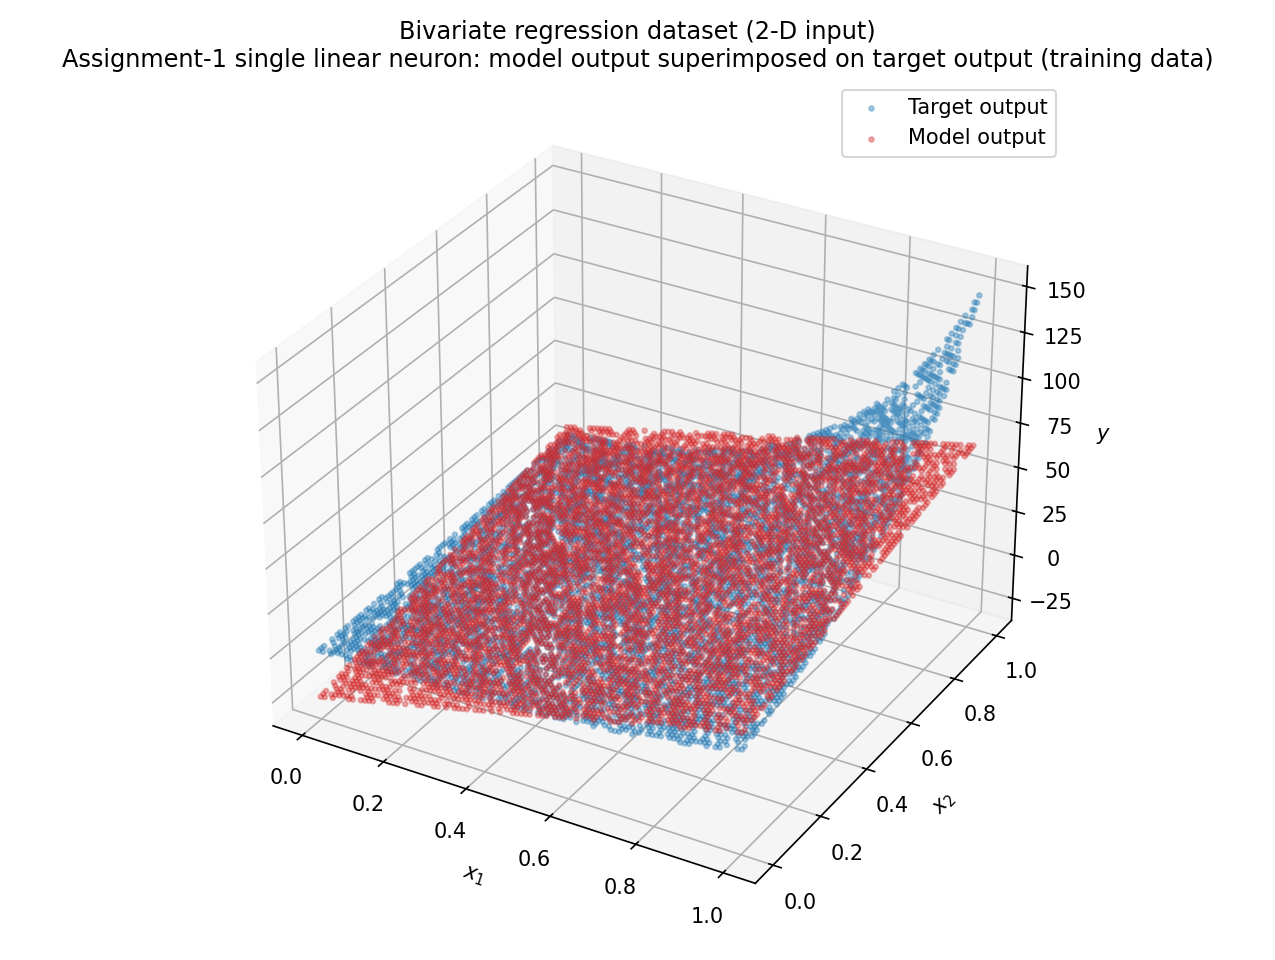
\includegraphics[width=0.8\textwidth,height=9.2cm,keepaspectratio]{figures/regression_bivariate__baseline_single_neuron_fit_train.png}
\caption{The Assignment-1 single linear neuron on the same training data.}
\end{figure}

\subsection{Inferences}
\begin{itemize}
  \item The selected architecture is 2-64-32-1, with a test RMSE of 0.1483 (0.73\% RMSE). Training, validation and test RMSE (0.1587 / 0.1416 / 0.1483) are almost identical, so the selected model generalises and is not overfitted.
  \item The comparison with Assignment-1 is decisive: the single linear neuron reaches a test RMSE of 11.5259 (56.51\%), so the FCNN reduces the test RMSE by 98.7\%. A single linear neuron can only represent a hyperplane, and the target function of this dataset is not linear, so its error is dominated by bias that no amount of further training can remove.
  \item Increasing the number of hidden nodes helps only up to a point. The worst validation RMSE among the architectures tried is 0.3361 (architecture 2-64-1) and the best is 0.1416; beyond the selected size the extra parameters do not lower the validation error, they only make the optimisation slower and noisier. This is the model-complexity trade-off the cross-validation step is meant to expose.
  \item The 3-D plot of model output superimposed on the target output shows the network surface following the target surface over the whole (x\textsubscript{1}, x\textsubscript{2}) domain, whereas the single linear neuron can only fit a flat plane through the same data.
  \item The target-vs-model scatter plots stay close to the diagonal for training, validation and test data; the small remaining spread is uniform across the output range rather than concentrated at the extremes.
  \item The hidden-node output plots show oriented sigmoid ramps over the (x\textsubscript{1}, x\textsubscript{2}) plane. With two hidden layers the second layer produces more localised surfaces, which is what lets the network model the curvature of the target surface with relatively few nodes.
  \item The assignment asks for both one and two hidden layers on this dataset. The best one-hidden-layer network is 2-16-1 (validation RMSE 0.1924, 65 weights) and the best two-hidden-layer network is 2-64-32-1 (validation RMSE 0.1416, 2305 weights), so the two-hidden-layer family wins here by 0.0508 RMSE - 2-64-32-1 against 2-16-1. The second hidden layer lets the network build more localised surfaces from the ridges produced by the first layer, which suits the curvature of this target function; note that it wins with a comparable, not a larger, parameter count, so the gain comes from the arrangement of the nodes rather than from sheer size.
  \item The average-error curve of the best architecture drops sharply in the first epochs and then decreases very slowly; it ran for 200 epochs. Because the weights are updated after every example, the curve is noticeably noisier than a batch-gradient-descent curve would be, which is the expected signature of SGD.
\end{itemize}

\clearpage

\section{Overall Observations and Conclusions}
\begin{itemize}
  \item \textbf{Nonlinear problems are where the FCNN pays off.} On the linearly separable classification dataset the FCNN and the Assignment-1 single neuron both reach 100.00\% test accuracy, so the extra capacity is unused. On the nonlinearly separable dataset the FCNN reaches 100.00\% against 92.67\% for the single neuron, and on the two regression datasets it reduces the test RMSE by 94.3\% and 98.7\% respectively.
  \item \textbf{Hidden nodes are feature detectors.} The hidden-node output plots show soft half-planes (classification) and ramps (regression); the output layer is a linear combination of those surfaces passed through the output activation. The number of hidden nodes therefore controls how many such surfaces are available, i.e. the capacity of the model.
  \item \textbf{More nodes is not better.} Validation accuracy / RMSE stops improving - and occasionally worsens - once the network is large enough. Selecting the architecture on validation data, and only then reporting on the test set, is what keeps the reported figures honest.
  \item \textbf{SGD behaves as expected.} The average-error curves fall steeply for the first few epochs and then flatten, and they are visibly noisy because the weights are updated after every single example. Standardising the inputs was necessary: with the raw inputs the logistic units saturate and the curves barely move.
  \item \textbf{Sensitivity to initialisation and to the optimisation run.} Performance is not monotone in the number of parameters. On the bivariate dataset, for example, 2-64-1 (257 weights) ends at a validation RMSE of 0.3361 while the smaller 2-16-1 (65 weights) reaches 0.1924 - the larger network can represent everything the smaller one can, so the gap is a property of the training run, not of the model. Squared error with logistic units has long flat regions, and plain SGD from a random start does not always escape them. This is a real limitation of the from-scratch setup and is why several architectures were trained and compared rather than one.
\end{itemize}

\end{document}
